\documentclass[a4paper]{book}
\usepackage{makeidx}
\usepackage{natbib}
\usepackage{graphicx}
\usepackage{multicol}
\usepackage{float}
\usepackage{listings}
\usepackage{color}
\usepackage{ifthen}
\usepackage[table]{xcolor}
\usepackage{textcomp}
\usepackage{alltt}
\usepackage{ifpdf}
\ifpdf
\usepackage[pdftex,
            pagebackref=true,
            colorlinks=true,
            linkcolor=blue,
            unicode
           ]{hyperref}
\else
\usepackage[ps2pdf,
            pagebackref=true,
            colorlinks=true,
            linkcolor=blue,
            unicode
           ]{hyperref}
\usepackage{pspicture}
\fi
\usepackage[utf8]{inputenc}
\usepackage{mathptmx}
\usepackage[scaled=.90]{helvet}
\usepackage{courier}
\usepackage{sectsty}
\usepackage[titles]{tocloft}
\usepackage{doxygen}
\lstset{language=C++,inputencoding=utf8,basicstyle=\footnotesize,breaklines=true,breakatwhitespace=true,tabsize=8,numbers=left }
\makeindex
\setcounter{tocdepth}{3}
\renewcommand{\footrulewidth}{0.4pt}
\renewcommand{\familydefault}{\sfdefault}
\hfuzz=15pt
\setlength{\emergencystretch}{15pt}
\hbadness=750
\tolerance=750
\begin{document}
\hypersetup{pageanchor=false,citecolor=blue}
\begin{titlepage}
\vspace*{7cm}
\begin{center}
{\Large \-My \-Project }\\
\vspace*{1cm}
{\large \-Generated by Doxygen 1.7.6.1}\\
\vspace*{0.5cm}
{\small Sun Apr 13 2014 22:22:45}\\
\end{center}
\end{titlepage}
\clearemptydoublepage
\pagenumbering{roman}
\tableofcontents
\clearemptydoublepage
\pagenumbering{arabic}
\hypersetup{pageanchor=true,citecolor=blue}
\chapter{\-Namespace \-Index}
\section{Namespace List}
Here is a list of all documented namespaces with brief descriptions:\begin{DoxyCompactList}
\item\contentsline{section}{\hyperlink{namespaceCL}{CL} (Control equation )}{\pageref{namespaceCL}}{}
\item\contentsline{section}{\hyperlink{namespaceCL_1_1Input}{CL::Input} (Abstract classes indicating controller input )}{\pageref{namespaceCL_1_1Input}}{}
\item\contentsline{section}{\hyperlink{namespaceCL_1_1Output}{CL::Output} (Abstract classes indicating controller output )}{\pageref{namespaceCL_1_1Output}}{}
\item\contentsline{section}{\hyperlink{namespaceInput}{Input} (Classes providing reference values to the controller )}{\pageref{namespaceInput}}{}
\item\contentsline{section}{\hyperlink{namespaceInput_1_1Vec3}{Input::Vec3} (Returning 3-\/element vector )}{\pageref{namespaceInput_1_1Vec3}}{}
\end{DoxyCompactList}

\chapter{\-Class \-Index}
\section{Class Hierarchy}
This inheritance list is sorted roughly, but not completely, alphabetically:\begin{DoxyCompactList}
\item \contentsline{section}{Array$<$ T $>$}{\pageref{classArray}}{}
\item \contentsline{section}{Array$<$ math::quat $>$}{\pageref{classArray}}{}
\item \contentsline{section}{Array$<$ math::vec3 $>$}{\pageref{classArray}}{}
\item \contentsline{section}{Attitude}{\pageref{classAttitude}}{}
\item \contentsline{section}{Input::Vec3::Base}{\pageref{classInput_1_1Vec3_1_1Base}}{}
\begin{DoxyCompactList}
\item \contentsline{section}{Input::Vec3::Circle}{\pageref{classInput_1_1Vec3_1_1Circle}}{}
\item \contentsline{section}{Input::Vec3::Const}{\pageref{classInput_1_1Vec3_1_1Const}}{}
\end{DoxyCompactList}
\item \contentsline{section}{CL::Base}{\pageref{classCL_1_1Base}}{}
\begin{DoxyCompactList}
\item \contentsline{section}{CL::Alpha}{\pageref{classCL_1_1Alpha}}{}
\begin{DoxyCompactList}
\item \contentsline{section}{Alpha1::Base}{\pageref{classAlpha1_1_1Base}}{}
\begin{DoxyCompactList}
\item \contentsline{section}{Alpha1::Omega}{\pageref{classAlpha1_1_1Omega}}{}
\begin{DoxyCompactList}
\item \contentsline{section}{Jerk::Base}{\pageref{classJerk_1_1Base}}{}
\begin{DoxyCompactList}
\item \contentsline{section}{Jerk::X}{\pageref{classJerk_1_1X}}{}
\end{DoxyCompactList}
\end{DoxyCompactList}
\item \contentsline{section}{Alpha1::Q}{\pageref{classAlpha1_1_1Q}}{}
\end{DoxyCompactList}
\item \contentsline{section}{Jounce::Base}{\pageref{classJounce_1_1Base}}{}
\begin{DoxyCompactList}
\item \contentsline{section}{Jounce::V}{\pageref{classJounce_1_1V}}{}
\item \contentsline{section}{Jounce::X}{\pageref{classJounce_1_1X}}{}
\end{DoxyCompactList}
\end{DoxyCompactList}
\item \contentsline{section}{CL::Omega$<$ N $>$}{\pageref{classCL_1_1Omega}}{}
\item \contentsline{section}{CL::Q$<$ N $>$}{\pageref{classCL_1_1Q}}{}
\item \contentsline{section}{CL::Thrust}{\pageref{classCL_1_1Thrust}}{}
\begin{DoxyCompactList}
\item \contentsline{section}{Jerk::Base}{\pageref{classJerk_1_1Base}}{}
\item \contentsline{section}{Jounce::Base}{\pageref{classJounce_1_1Base}}{}
\end{DoxyCompactList}
\item \contentsline{section}{CL::V$<$ N $>$}{\pageref{classCL_1_1V}}{}
\item \contentsline{section}{CL::X$<$ N $>$}{\pageref{classCL_1_1X}}{}
\item \contentsline{section}{CL::Omega$<$ 2 $>$}{\pageref{classCL_1_1Omega}}{}
\begin{DoxyCompactList}
\item \contentsline{section}{Alpha1::Omega}{\pageref{classAlpha1_1_1Omega}}{}
\end{DoxyCompactList}
\item \contentsline{section}{CL::Q$<$ 2 $>$}{\pageref{classCL_1_1Q}}{}
\begin{DoxyCompactList}
\item \contentsline{section}{Alpha1::Q}{\pageref{classAlpha1_1_1Q}}{}
\end{DoxyCompactList}
\item \contentsline{section}{CL::V$<$ 4 $>$}{\pageref{classCL_1_1V}}{}
\begin{DoxyCompactList}
\item \contentsline{section}{Jounce::V}{\pageref{classJounce_1_1V}}{}
\end{DoxyCompactList}
\item \contentsline{section}{CL::X$<$ 4 $>$}{\pageref{classCL_1_1X}}{}
\begin{DoxyCompactList}
\item \contentsline{section}{Jerk::X}{\pageref{classJerk_1_1X}}{}
\end{DoxyCompactList}
\item \contentsline{section}{CL::X$<$ 5 $>$}{\pageref{classCL_1_1X}}{}
\begin{DoxyCompactList}
\item \contentsline{section}{Jounce::X}{\pageref{classJounce_1_1X}}{}
\end{DoxyCompactList}
\end{DoxyCompactList}
\item \contentsline{section}{Command::Base}{\pageref{classCommand_1_1Base}}{}
\begin{DoxyCompactList}
\item \contentsline{section}{Command::Freeze}{\pageref{classCommand_1_1Freeze}}{}
\item \contentsline{section}{Command::Q}{\pageref{classCommand_1_1Q}}{}
\item \contentsline{section}{Command::V}{\pageref{classCommand_1_1V}}{}
\item \contentsline{section}{Command::X}{\pageref{classCommand_1_1X}}{}
\end{DoxyCompactList}
\item \contentsline{section}{Command::Stop::Base}{\pageref{classCommand_1_1Stop_1_1Base}}{}
\begin{DoxyCompactList}
\item \contentsline{section}{Command::Stop::QSettle}{\pageref{classCommand_1_1Stop_1_1QSettle}}{}
\item \contentsline{section}{Command::Stop::Time}{\pageref{classCommand_1_1Stop_1_1Time}}{}
\item \contentsline{section}{Command::Stop::VCross}{\pageref{classCommand_1_1Stop_1_1VCross}}{}
\item \contentsline{section}{Command::Stop::VSettle}{\pageref{classCommand_1_1Stop_1_1VSettle}}{}
\item \contentsline{section}{Command::Stop::XCross}{\pageref{classCommand_1_1Stop_1_1XCross}}{}
\item \contentsline{section}{Command::Stop::XSettle}{\pageref{classCommand_1_1Stop_1_1XSettle}}{}
\end{DoxyCompactList}
\item \contentsline{section}{Brain}{\pageref{classBrain}}{}
\item \contentsline{section}{Command::Base::Flag}{\pageref{structCommand_1_1Base_1_1Flag}}{}
\item \contentsline{section}{Brain::Mode}{\pageref{structBrain_1_1Mode}}{}
\item \contentsline{section}{Attitude::Mode}{\pageref{structAttitude_1_1Mode}}{}
\item \contentsline{section}{Plant}{\pageref{classPlant}}{}
\item \contentsline{section}{Position}{\pageref{classPosition}}{}
\item \contentsline{section}{Quadrotor}{\pageref{classQuadrotor}}{}
\item \contentsline{section}{Input::Quat}{\pageref{classInput_1_1Quat}}{}
\begin{DoxyCompactList}
\item \contentsline{section}{Input::QuatConst}{\pageref{classInput_1_1QuatConst}}{}
\end{DoxyCompactList}
\item \contentsline{section}{StopCond}{\pageref{classStopCond}}{}
\begin{DoxyCompactList}
\item \contentsline{section}{EmptyQueue}{\pageref{classEmptyQueue}}{}
\item \contentsline{section}{Inf}{\pageref{classInf}}{}
\item \contentsline{section}{InvalidOp}{\pageref{classInvalidOp}}{}
\item \contentsline{section}{OmegaHigh}{\pageref{classOmegaHigh}}{}
\end{DoxyCompactList}
\item \contentsline{section}{Telem}{\pageref{classTelem}}{}
\item \contentsline{section}{CL::Terms$<$ N $>$}{\pageref{classCL_1_1Terms}}{}
\begin{DoxyCompactList}
\item \contentsline{section}{CL::Omega$<$ N $>$}{\pageref{classCL_1_1Omega}}{}
\item \contentsline{section}{CL::V$<$ N $>$}{\pageref{classCL_1_1V}}{}
\item \contentsline{section}{CL::X$<$ N $>$}{\pageref{classCL_1_1X}}{}
\item \contentsline{section}{CL::Omega$<$ 2 $>$}{\pageref{classCL_1_1Omega}}{}
\item \contentsline{section}{CL::V$<$ 4 $>$}{\pageref{classCL_1_1V}}{}
\item \contentsline{section}{CL::X$<$ 4 $>$}{\pageref{classCL_1_1X}}{}
\item \contentsline{section}{CL::X$<$ 5 $>$}{\pageref{classCL_1_1X}}{}
\end{DoxyCompactList}
\item \contentsline{section}{CL::Terms$<$ N+1 $>$}{\pageref{classCL_1_1Terms}}{}
\begin{DoxyCompactList}
\item \contentsline{section}{CL::Q$<$ N $>$}{\pageref{classCL_1_1Q}}{}
\item \contentsline{section}{CL::Q$<$ 2 $>$}{\pageref{classCL_1_1Q}}{}
\end{DoxyCompactList}
\item \contentsline{section}{Command::Base::Type}{\pageref{structCommand_1_1Base_1_1Type}}{}
\end{DoxyCompactList}

\chapter{\-Class \-Index}
\section{Class List}
Here are the classes, structs, unions and interfaces with brief descriptions:\begin{DoxyCompactList}
\item\contentsline{section}{\hyperlink{classCL_1_1Alpha}{CL::Alpha} }{\pageref{classCL_1_1Alpha}}{}
\item\contentsline{section}{\hyperlink{classArray}{Array$<$ T $>$} }{\pageref{classArray}}{}
\item\contentsline{section}{\hyperlink{classAttitude}{Attitude} }{\pageref{classAttitude}}{}
\item\contentsline{section}{\hyperlink{classJerk_1_1Base}{Jerk::Base} }{\pageref{classJerk_1_1Base}}{}
\item\contentsline{section}{\hyperlink{classJounce_1_1Base}{Jounce::Base} }{\pageref{classJounce_1_1Base}}{}
\item\contentsline{section}{\hyperlink{classAlpha1_1_1Base}{Alpha1::Base} }{\pageref{classAlpha1_1_1Base}}{}
\item\contentsline{section}{\hyperlink{classInput_1_1Vec3_1_1Base}{Input::Vec3::Base} }{\pageref{classInput_1_1Vec3_1_1Base}}{}
\item\contentsline{section}{\hyperlink{classCL_1_1Base}{CL::Base} }{\pageref{classCL_1_1Base}}{}
\item\contentsline{section}{\hyperlink{classCommand_1_1Base}{Command::Base} }{\pageref{classCommand_1_1Base}}{}
\item\contentsline{section}{\hyperlink{classCommand_1_1Stop_1_1Base}{Command::Stop::Base} }{\pageref{classCommand_1_1Stop_1_1Base}}{}
\item\contentsline{section}{\hyperlink{classBrain}{Brain} }{\pageref{classBrain}}{}
\item\contentsline{section}{\hyperlink{classInput_1_1Vec3_1_1Circle}{Input::Vec3::Circle} }{\pageref{classInput_1_1Vec3_1_1Circle}}{}
\item\contentsline{section}{\hyperlink{classInput_1_1Vec3_1_1Const}{Input::Vec3::Const} }{\pageref{classInput_1_1Vec3_1_1Const}}{}
\item\contentsline{section}{\hyperlink{classEmptyQueue}{EmptyQueue} }{\pageref{classEmptyQueue}}{}
\item\contentsline{section}{\hyperlink{structCommand_1_1Base_1_1Flag}{Command::Base::Flag} }{\pageref{structCommand_1_1Base_1_1Flag}}{}
\item\contentsline{section}{\hyperlink{classCommand_1_1Freeze}{Command::Freeze} }{\pageref{classCommand_1_1Freeze}}{}
\item\contentsline{section}{\hyperlink{classInf}{Inf} }{\pageref{classInf}}{}
\item\contentsline{section}{\hyperlink{classInvalidOp}{InvalidOp} }{\pageref{classInvalidOp}}{}
\item\contentsline{section}{\hyperlink{structBrain_1_1Mode}{Brain::Mode} }{\pageref{structBrain_1_1Mode}}{}
\item\contentsline{section}{\hyperlink{structAttitude_1_1Mode}{Attitude::Mode} }{\pageref{structAttitude_1_1Mode}}{}
\item\contentsline{section}{\hyperlink{classAlpha1_1_1Omega}{Alpha1::Omega} }{\pageref{classAlpha1_1_1Omega}}{}
\item\contentsline{section}{\hyperlink{classCL_1_1Omega}{CL::Omega$<$ N $>$} }{\pageref{classCL_1_1Omega}}{}
\item\contentsline{section}{\hyperlink{classOmegaHigh}{OmegaHigh} }{\pageref{classOmegaHigh}}{}
\item\contentsline{section}{\hyperlink{classPlant}{Plant} }{\pageref{classPlant}}{}
\item\contentsline{section}{\hyperlink{classPosition}{Position} }{\pageref{classPosition}}{}
\item\contentsline{section}{\hyperlink{classCommand_1_1Q}{Command::Q} }{\pageref{classCommand_1_1Q}}{}
\item\contentsline{section}{\hyperlink{classAlpha1_1_1Q}{Alpha1::Q} }{\pageref{classAlpha1_1_1Q}}{}
\item\contentsline{section}{\hyperlink{classCL_1_1Q}{CL::Q$<$ N $>$} }{\pageref{classCL_1_1Q}}{}
\item\contentsline{section}{\hyperlink{classCommand_1_1Stop_1_1QSettle}{Command::Stop::QSettle} }{\pageref{classCommand_1_1Stop_1_1QSettle}}{}
\item\contentsline{section}{\hyperlink{classQuadrotor}{Quadrotor} }{\pageref{classQuadrotor}}{}
\item\contentsline{section}{\hyperlink{classInput_1_1Quat}{Input::Quat} }{\pageref{classInput_1_1Quat}}{}
\item\contentsline{section}{\hyperlink{classInput_1_1QuatConst}{Input::QuatConst} }{\pageref{classInput_1_1QuatConst}}{}
\item\contentsline{section}{\hyperlink{classStopCond}{StopCond} }{\pageref{classStopCond}}{}
\item\contentsline{section}{\hyperlink{classTelem}{Telem} }{\pageref{classTelem}}{}
\item\contentsline{section}{\hyperlink{classCL_1_1Terms}{CL::Terms$<$ N $>$} }{\pageref{classCL_1_1Terms}}{}
\item\contentsline{section}{\hyperlink{classCL_1_1Thrust}{CL::Thrust} }{\pageref{classCL_1_1Thrust}}{}
\item\contentsline{section}{\hyperlink{classCommand_1_1Stop_1_1Time}{Command::Stop::Time} }{\pageref{classCommand_1_1Stop_1_1Time}}{}
\item\contentsline{section}{\hyperlink{structCommand_1_1Base_1_1Type}{Command::Base::Type} }{\pageref{structCommand_1_1Base_1_1Type}}{}
\item\contentsline{section}{\hyperlink{classCL_1_1V}{CL::V$<$ N $>$} }{\pageref{classCL_1_1V}}{}
\item\contentsline{section}{\hyperlink{classCommand_1_1V}{Command::V} }{\pageref{classCommand_1_1V}}{}
\item\contentsline{section}{\hyperlink{classJounce_1_1V}{Jounce::V} }{\pageref{classJounce_1_1V}}{}
\item\contentsline{section}{\hyperlink{classCommand_1_1Stop_1_1VCross}{Command::Stop::VCross} }{\pageref{classCommand_1_1Stop_1_1VCross}}{}
\item\contentsline{section}{\hyperlink{classCommand_1_1Stop_1_1VSettle}{Command::Stop::VSettle} }{\pageref{classCommand_1_1Stop_1_1VSettle}}{}
\item\contentsline{section}{\hyperlink{classJerk_1_1X}{Jerk::X} }{\pageref{classJerk_1_1X}}{}
\item\contentsline{section}{\hyperlink{classJounce_1_1X}{Jounce::X} }{\pageref{classJounce_1_1X}}{}
\item\contentsline{section}{\hyperlink{classCL_1_1X}{CL::X$<$ N $>$} }{\pageref{classCL_1_1X}}{}
\item\contentsline{section}{\hyperlink{classCommand_1_1X}{Command::X} }{\pageref{classCommand_1_1X}}{}
\item\contentsline{section}{\hyperlink{classCommand_1_1Stop_1_1XCross}{Command::Stop::XCross} }{\pageref{classCommand_1_1Stop_1_1XCross}}{}
\item\contentsline{section}{\hyperlink{classCommand_1_1Stop_1_1XSettle}{Command::Stop::XSettle} }{\pageref{classCommand_1_1Stop_1_1XSettle}}{}
\end{DoxyCompactList}

\chapter{\-Namespace \-Documentation}
\hypertarget{namespaceCL}{
\section{CL Namespace Reference}
\label{namespaceCL}\index{CL@{CL}}
}


Control equation.  
\subsection*{Namespaces}
\begin{DoxyCompactItemize}
\item 
namespace \hyperlink{namespaceCL_1_1Input}{Input}


\begin{DoxyCompactList}\small\item\em Abstract classes indicating controller input. \item\end{DoxyCompactList}\item 
namespace \hyperlink{namespaceCL_1_1Output}{Output}


\begin{DoxyCompactList}\small\item\em Abstract classes indicating controller output. \item\end{DoxyCompactList}\end{DoxyCompactItemize}
\subsection*{Classes}
\begin{DoxyCompactItemize}
\item 
class \hyperlink{classCL_1_1Base}{Base}
\item 
class \hyperlink{classCL_1_1Terms}{Terms}
\item 
class \hyperlink{classCL_1_1X}{X}
\item 
class \hyperlink{classCL_1_1V}{V}
\item 
class \hyperlink{classCL_1_1Q}{Q}
\item 
class \hyperlink{classCL_1_1Omega}{Omega}
\item 
class \hyperlink{classCL_1_1Thrust}{Thrust}
\item 
class \hyperlink{classCL_1_1Alpha}{Alpha}
\end{DoxyCompactItemize}


\subsection{Detailed Description}
Control equation. 
\hypertarget{namespaceCL_1_1Input}{\section{\-C\-L\-:\-:\-Input \-Namespace \-Reference}
\label{namespaceCL_1_1Input}\index{\-C\-L\-::\-Input@{\-C\-L\-::\-Input}}
}


\-Abstract classes indicating controller input.  




\subsection{\-Detailed \-Description}
\-Abstract classes indicating controller input. 
\hypertarget{namespaceCL_1_1Output}{
\section{CL::Output Namespace Reference}
\label{namespaceCL_1_1Output}\index{CL::Output@{CL::Output}}
}


Abstract classes indicating controller output.  


\subsection{Detailed Description}
Abstract classes indicating controller output. 
\hypertarget{namespaceInput}{
\section{Input Namespace Reference}
\label{namespaceInput}\index{Input@{Input}}
}


Classes providing reference values to the controller.  
\subsection*{Namespaces}
\begin{DoxyCompactItemize}
\item 
namespace \hyperlink{namespaceInput_1_1Vec3}{Vec3}


\begin{DoxyCompactList}\small\item\em Returning 3-\/element vector. \item\end{DoxyCompactList}\end{DoxyCompactItemize}
\subsection*{Classes}
\begin{DoxyCompactItemize}
\item 
class \hyperlink{classInput_1_1Quat}{Quat}
\item 
class \hyperlink{classInput_1_1QuatConst}{QuatConst}
\end{DoxyCompactItemize}


\subsection{Detailed Description}
Classes providing reference values to the controller. 
\hypertarget{namespaceInput_1_1Vec3}{\section{\-Input\-:\-:\-Vec3 \-Namespace \-Reference}
\label{namespaceInput_1_1Vec3}\index{\-Input\-::\-Vec3@{\-Input\-::\-Vec3}}
}


\-Returning 3-\/element vector.  


\subsection*{\-Classes}
\begin{DoxyCompactItemize}
\item 
class \hyperlink{classInput_1_1Vec3_1_1Base}{\-Base}
\item 
class \hyperlink{classInput_1_1Vec3_1_1Const}{\-Const}
\item 
class \hyperlink{classInput_1_1Vec3_1_1Circle}{\-Circle}
\end{DoxyCompactItemize}


\subsection{\-Detailed \-Description}
\-Returning 3-\/element vector. 
\chapter{\-Class \-Documentation}
\hypertarget{classCL_1_1Alpha}{\section{\-C\-L\-:\-:\-Alpha \-Class \-Reference}
\label{classCL_1_1Alpha}\index{\-C\-L\-::\-Alpha@{\-C\-L\-::\-Alpha}}
}


\-Inheritance diagram for \-C\-L\-:\-:\-Alpha\-:\nopagebreak
\begin{figure}[H]
\begin{center}
\leavevmode
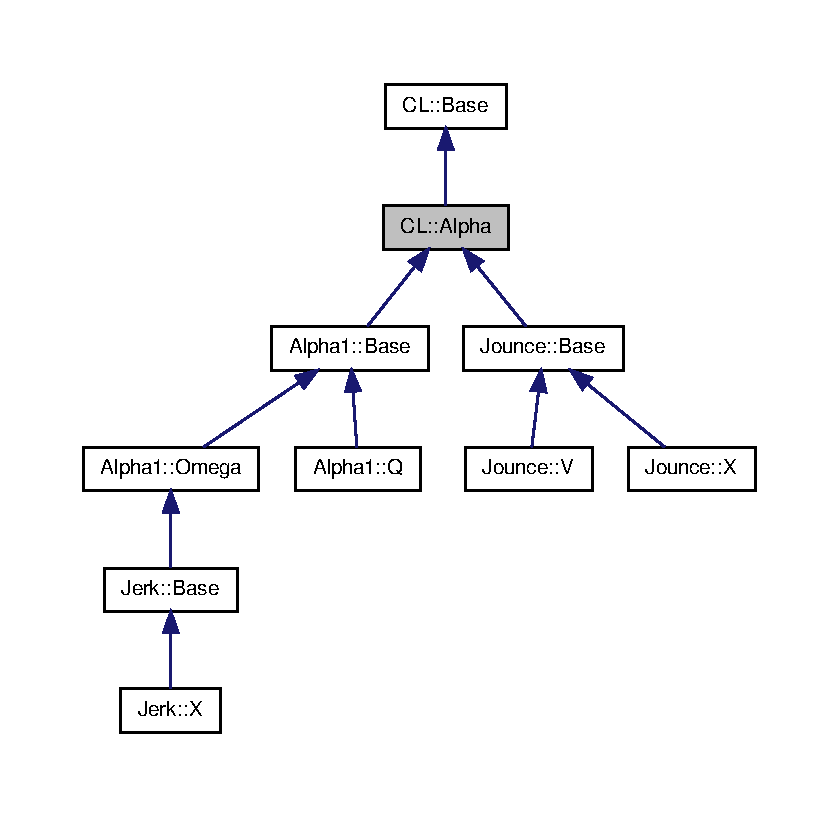
\includegraphics[width=350pt]{classCL_1_1Alpha__inherit__graph}
\end{center}
\end{figure}


\-Collaboration diagram for \-C\-L\-:\-:\-Alpha\-:\nopagebreak
\begin{figure}[H]
\begin{center}
\leavevmode
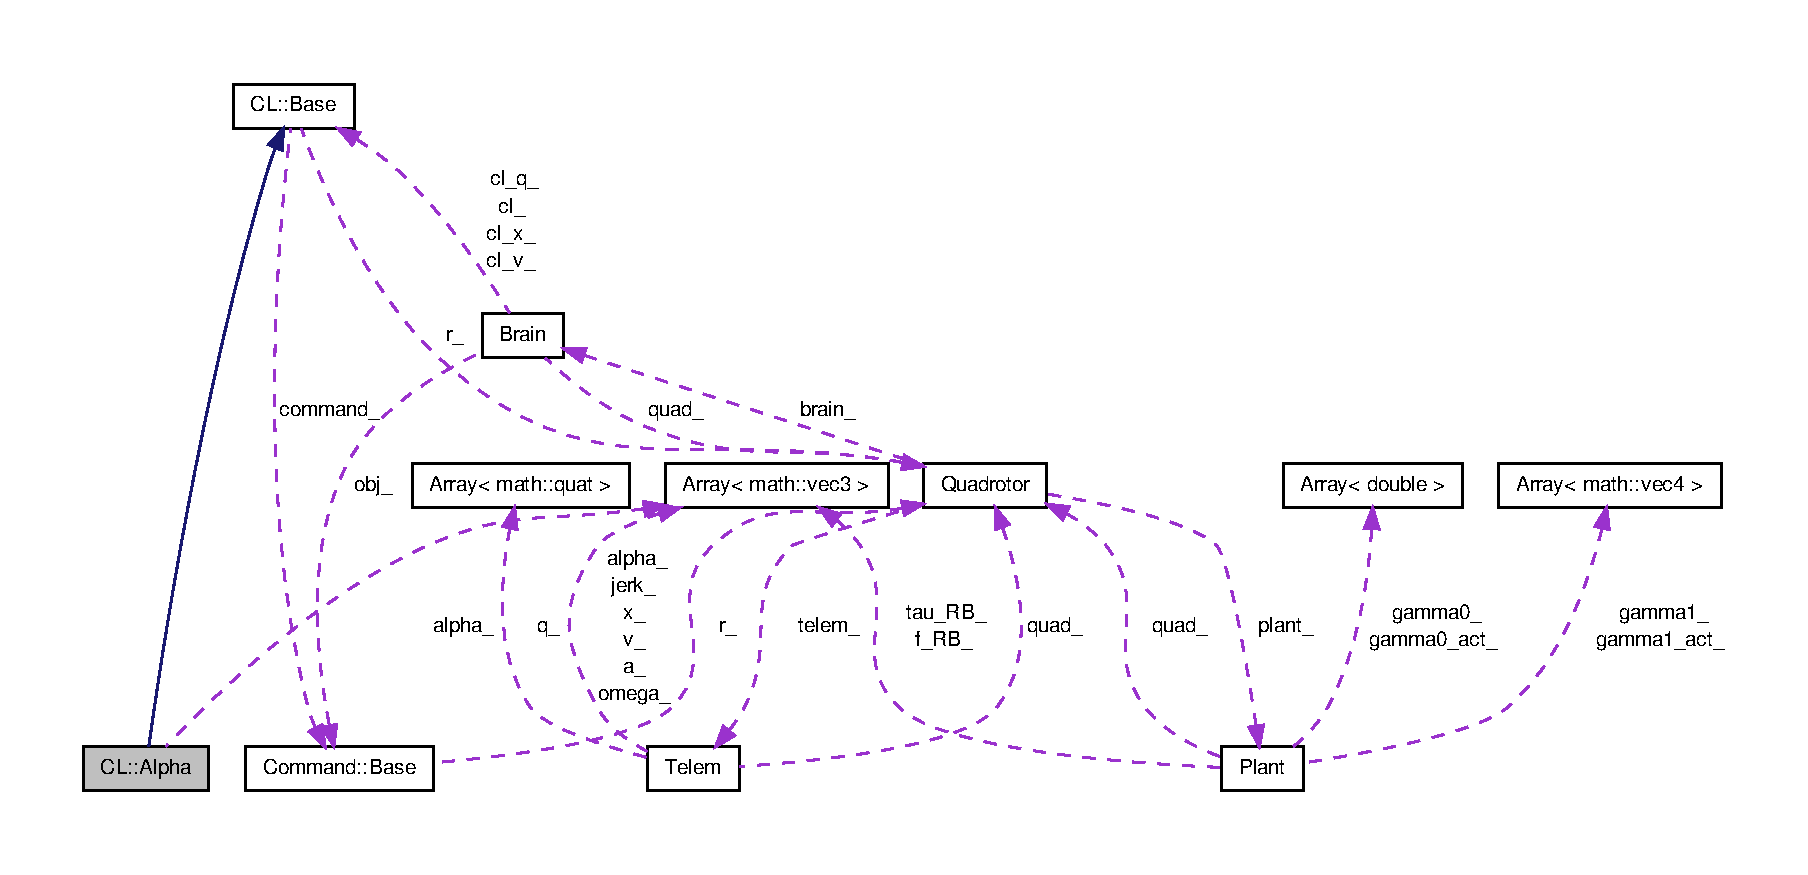
\includegraphics[width=350pt]{classCL_1_1Alpha__coll__graph}
\end{center}
\end{figure}
\subsection*{\-Public \-Member \-Functions}
\begin{DoxyCompactItemize}
\item 
\hypertarget{classCL_1_1Alpha_a7144b55588a6fdd8d6e6270230c510a5}{{\bfseries \-Alpha} (\hyperlink{classQuadrotor}{\-Quadrotor} $\ast$r)}\label{classCL_1_1Alpha_a7144b55588a6fdd8d6e6270230c510a5}

\item 
\hypertarget{classCL_1_1Alpha_a3abee3653d7af651347097e67824151f}{virtual void {\bfseries \-Step} (int, double)}\label{classCL_1_1Alpha_a3abee3653d7af651347097e67824151f}

\item 
\hypertarget{classCL_1_1Alpha_a5425efcdfe00976a373a66fda1b51faa}{virtual void {\bfseries alloc} (int)}\label{classCL_1_1Alpha_a5425efcdfe00976a373a66fda1b51faa}

\item 
\hypertarget{classCL_1_1Alpha_a5c69fe1c1de2576c2db2c7724eaf909a}{virtual void {\bfseries write} (int)}\label{classCL_1_1Alpha_a5c69fe1c1de2576c2db2c7724eaf909a}

\end{DoxyCompactItemize}
\subsection*{\-Public \-Attributes}
\begin{DoxyCompactItemize}
\item 
\hypertarget{classCL_1_1Alpha_a27d343cf1970d5a561169bd8533d427b}{\hyperlink{classArray}{\-Array}$<$ math\-::vec3 $>$ {\bfseries alpha\-\_\-}}\label{classCL_1_1Alpha_a27d343cf1970d5a561169bd8533d427b}

\end{DoxyCompactItemize}


\-The documentation for this class was generated from the following files\-:\begin{DoxyCompactItemize}
\item 
src/quadrotor/\-Control\-Law/\-Control\-Law.\-h\item 
src/quadrotor/\-Control\-Law/\-Control\-Law.\-cpp\end{DoxyCompactItemize}

\hypertarget{classArray}{\section{\-Array$<$ \-T $>$ \-Class \-Template \-Reference}
\label{classArray}\index{\-Array$<$ T $>$@{\-Array$<$ T $>$}}
}


\-Collaboration diagram for \-Array$<$ \-T $>$\-:\nopagebreak
\begin{figure}[H]
\begin{center}
\leavevmode
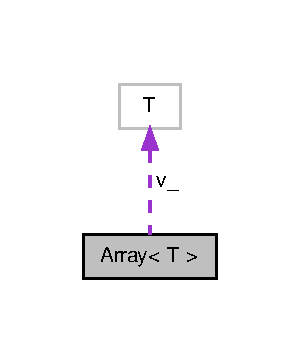
\includegraphics[width=144pt]{classArray__coll__graph}
\end{center}
\end{figure}
\subsection*{\-Public \-Member \-Functions}
\begin{DoxyCompactItemize}
\item 
\hypertarget{classArray_a590e6a7f6a10122acf677b5f7191e9ec}{void {\bfseries alloc} (int n)}\label{classArray_a590e6a7f6a10122acf677b5f7191e9ec}

\item 
\hypertarget{classArray_ae911195ae0ab8040c8780c6fc0a11b1b}{\-T \& {\bfseries operator\mbox{[}$\,$\mbox{]}} (int i)}\label{classArray_ae911195ae0ab8040c8780c6fc0a11b1b}

\item 
\hypertarget{classArray_a1980151be6d25c4d8acaaee358881a0d}{void {\bfseries write} (\-F\-I\-L\-E $\ast$file, int n)}\label{classArray_a1980151be6d25c4d8acaaee358881a0d}

\item 
\hypertarget{classArray_a728430d7e0933b1ab4607ba98255c2ef}{void {\bfseries read} (\-F\-I\-L\-E $\ast$file, int n)}\label{classArray_a728430d7e0933b1ab4607ba98255c2ef}

\item 
\hypertarget{classArray_a3e395a7a0ba33776744d7af2c387ebd8}{void {\bfseries fill} (\-T const \&t)}\label{classArray_a3e395a7a0ba33776744d7af2c387ebd8}

\end{DoxyCompactItemize}
\subsection*{\-Public \-Attributes}
\begin{DoxyCompactItemize}
\item 
\hypertarget{classArray_ac6494b108f60fb2d80ab65d7bb75390a}{int {\bfseries n\-\_\-}}\label{classArray_ac6494b108f60fb2d80ab65d7bb75390a}

\item 
\hypertarget{classArray_af7695e08563d3f4454f1213ca0d7b88a}{\-T $\ast$ {\bfseries v\-\_\-}}\label{classArray_af7695e08563d3f4454f1213ca0d7b88a}

\end{DoxyCompactItemize}
\subsubsection*{template$<$typename \-T$>$ class Array$<$ T $>$}



\-The documentation for this class was generated from the following file\-:\begin{DoxyCompactItemize}
\item 
src/quadrotor/array.\-h\end{DoxyCompactItemize}

\hypertarget{classAttitude}{
\section{Attitude Class Reference}
\label{classAttitude}\index{Attitude@{Attitude}}
}
Collaboration diagram for Attitude:\subsection*{Classes}
\begin{DoxyCompactItemize}
\item 
struct \hyperlink{structAttitude_1_1Mode}{Mode}
\end{DoxyCompactItemize}
\subsection*{Public Member Functions}
\begin{DoxyCompactItemize}
\item 
\hypertarget{classAttitude_a3d8702ddb8ebe640b4dae5d2a13415c7}{
{\bfseries Attitude} (\hyperlink{classQuadrotor}{Quadrotor} $\ast$quad)}
\label{classAttitude_a3d8702ddb8ebe640b4dae5d2a13415c7}

\item 
\hypertarget{classAttitude_a7e04169ea1c1b522a529c2c175cf73e7}{
void {\bfseries reset} ()}
\label{classAttitude_a7e04169ea1c1b522a529c2c175cf73e7}

\item 
\hypertarget{classAttitude_a8b8e86dce3952d51a2b31bdb19922f20}{
void {\bfseries set\_\-q\_\-reference} (int ti, math::quat q)}
\label{classAttitude_a8b8e86dce3952d51a2b31bdb19922f20}

\item 
\hypertarget{classAttitude_adb83854056302fbda19b037da086f839}{
void {\bfseries set\_\-o\_\-reference} (int ti, math::vec3 o)}
\label{classAttitude_adb83854056302fbda19b037da086f839}

\item 
\hypertarget{classAttitude_a9bc858b7855f4f3ea2b405759c34e6ec}{
void {\bfseries set\_\-o\_\-reference} (int ti, double, double, double)}
\label{classAttitude_a9bc858b7855f4f3ea2b405759c34e6ec}

\item 
\hypertarget{classAttitude_ac718a7f20470355bb45d1c14ef266d95}{
void {\bfseries set\_\-obj} (int ti1, Command::Orient $\ast$att)}
\label{classAttitude_ac718a7f20470355bb45d1c14ef266d95}

\item 
\hypertarget{classAttitude_a9d2850ba4bc838cf06907a351004bf13}{
void {\bfseries step} (double dt, int ti, int ti\_\-0)}
\label{classAttitude_a9d2850ba4bc838cf06907a351004bf13}

\item 
\hypertarget{classAttitude_ad611f128c6a7d4cbb0f52fad22dc7c98}{
void {\bfseries step\_\-torque\_\-rotor\_\-body} (int ti, int ti\_\-0)}
\label{classAttitude_ad611f128c6a7d4cbb0f52fad22dc7c98}

\item 
\hypertarget{classAttitude_a96c6947c3d191036db56a103e1a01f4d}{
void {\bfseries step\_\-torque\_\-rotor\_\-body\_\-att} (int ti, int ti\_\-0)}
\label{classAttitude_a96c6947c3d191036db56a103e1a01f4d}

\item 
\hypertarget{classAttitude_a3acffc90c62c76fe37ce352e090f804f}{
void {\bfseries step\_\-torque\_\-rotor\_\-body\_\-vel} (int ti, int ti\_\-0)}
\label{classAttitude_a3acffc90c62c76fe37ce352e090f804f}

\item 
\hypertarget{classAttitude_a303e24774c3086915d85803be88a5e27}{
void {\bfseries step\_\-torque\_\-rotor\_\-body} (int, math::vec3)}
\label{classAttitude_a303e24774c3086915d85803be88a5e27}

\item 
\hypertarget{classAttitude_a8e46df6befc26497fe52c7a727da2154}{
void {\bfseries write} (int n=0)}
\label{classAttitude_a8e46df6befc26497fe52c7a727da2154}

\item 
\hypertarget{classAttitude_a82ea007a5d6b22c5016308b982816459}{
void {\bfseries write\_\-param} ()}
\label{classAttitude_a82ea007a5d6b22c5016308b982816459}

\item 
\hypertarget{classAttitude_a628672fe0bc80ab2451362a519bfc81f}{
void {\bfseries read\_\-param} ()}
\label{classAttitude_a628672fe0bc80ab2451362a519bfc81f}

\end{DoxyCompactItemize}
\subsection*{Public Attributes}
\begin{DoxyCompactItemize}
\item 
\hypertarget{classAttitude_a0f341afa94379e3eb7619782d33e2690}{
unsigned int {\bfseries mode\_\-}}
\label{classAttitude_a0f341afa94379e3eb7619782d33e2690}

\item 
\hypertarget{classAttitude_a46e4a1fd13d48a7811ca925f8a33d7a3}{
\hyperlink{classQuadrotor}{Quadrotor} $\ast$ {\bfseries quad\_\-}}
\label{classAttitude_a46e4a1fd13d48a7811ca925f8a33d7a3}

\item 
\hypertarget{classAttitude_a902c2fc6c510aa1eca73c812854a4531}{
Command::Orient $\ast$ {\bfseries att\_\-}}
\label{classAttitude_a902c2fc6c510aa1eca73c812854a4531}

\item 
\hypertarget{classAttitude_a4551548f9b888cbc3f4a41d102fea01f}{
math::mat33 {\bfseries C1\_\-}}
\label{classAttitude_a4551548f9b888cbc3f4a41d102fea01f}

\item 
\hypertarget{classAttitude_a6e00c25cca6bf99d4828c96e22dd0f85}{
math::mat33 {\bfseries C2\_\-}}
\label{classAttitude_a6e00c25cca6bf99d4828c96e22dd0f85}

\item 
\hypertarget{classAttitude_a8117974c86248890c7c7ab6db5c73966}{
\hyperlink{classArray}{Array}$<$ math::quat $>$ {\bfseries e1\_\-}}
\label{classAttitude_a8117974c86248890c7c7ab6db5c73966}

\item 
\hypertarget{classAttitude_accfe50fd0abccd801da3708cd68e4896}{
\hyperlink{classArray}{Array}$<$ math::vec3 $>$ {\bfseries e2\_\-}}
\label{classAttitude_accfe50fd0abccd801da3708cd68e4896}

\item 
\hypertarget{classAttitude_aeec79b62c3e4e703e1f902bd989ee0ea}{
\hyperlink{classArray}{Array}$<$ math::quat $>$ {\bfseries q\_\-ref\_\-}}
\label{classAttitude_aeec79b62c3e4e703e1f902bd989ee0ea}

\item 
\hypertarget{classAttitude_a5d15fad5ac2ee69a8b1a306b33d7bcb8}{
\hyperlink{classArray}{Array}$<$ math::vec3 $>$ {\bfseries q\_\-ref\_\-d\_\-}}
\label{classAttitude_a5d15fad5ac2ee69a8b1a306b33d7bcb8}

\item 
\hypertarget{classAttitude_adafdcc5ea0edf640443a54e0a1c8195e}{
\hyperlink{classArray}{Array}$<$ math::vec3 $>$ {\bfseries q\_\-ref\_\-dd\_\-}}
\label{classAttitude_adafdcc5ea0edf640443a54e0a1c8195e}

\item 
\hypertarget{classAttitude_a07ff1dc9f3a307aaa7744c4cc18b85b2}{
\hyperlink{classArray}{Array}$<$ math::vec3 $>$ {\bfseries o\_\-ref\_\-}}
\label{classAttitude_a07ff1dc9f3a307aaa7744c4cc18b85b2}

\item 
\hypertarget{classAttitude_ada75e65bfb26b7656e76cbd5500d2a66}{
\hyperlink{classArray}{Array}$<$ math::vec3 $>$ {\bfseries o\_\-ref\_\-d\_\-}}
\label{classAttitude_ada75e65bfb26b7656e76cbd5500d2a66}

\item 
\hypertarget{classAttitude_a96f44c3ffba76b9cc233fca1727b23ff}{
\hyperlink{classArray}{Array}$<$ double $>$ {\bfseries e1\_\-mag\_\-}}
\label{classAttitude_a96f44c3ffba76b9cc233fca1727b23ff}

\item 
\hypertarget{classAttitude_a45e77bc2aa5f7f449ea6d813465b6390}{
\hyperlink{classArray}{Array}$<$ double $>$ {\bfseries e1\_\-mag\_\-d\_\-}}
\label{classAttitude_a45e77bc2aa5f7f449ea6d813465b6390}

\item 
\hypertarget{classAttitude_ac1877b6ed64892ddcffc95e95591b484}{
\hyperlink{classArray}{Array}$<$ math::vec3 $>$ {\bfseries tau\_\-RB\_\-}}
\label{classAttitude_ac1877b6ed64892ddcffc95e95591b484}

\end{DoxyCompactItemize}


The documentation for this class was generated from the following files:\begin{DoxyCompactItemize}
\item 
src/quadrotor/attitude.h\item 
src/quadrotor/attitude.cpp\end{DoxyCompactItemize}

\hypertarget{classJerk_1_1Base}{\section{\-Jerk\-:\-:\-Base \-Class \-Reference}
\label{classJerk_1_1Base}\index{\-Jerk\-::\-Base@{\-Jerk\-::\-Base}}
}


\-Inheritance diagram for \-Jerk\-:\-:\-Base\-:\nopagebreak
\begin{figure}[H]
\begin{center}
\leavevmode
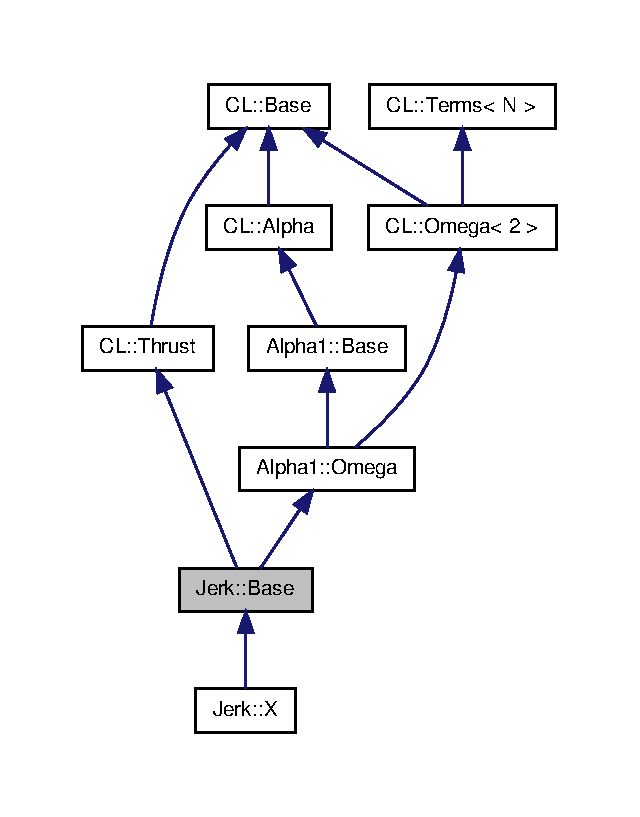
\includegraphics[width=307pt]{classJerk_1_1Base__inherit__graph}
\end{center}
\end{figure}


\-Collaboration diagram for \-Jerk\-:\-:\-Base\-:\nopagebreak
\begin{figure}[H]
\begin{center}
\leavevmode
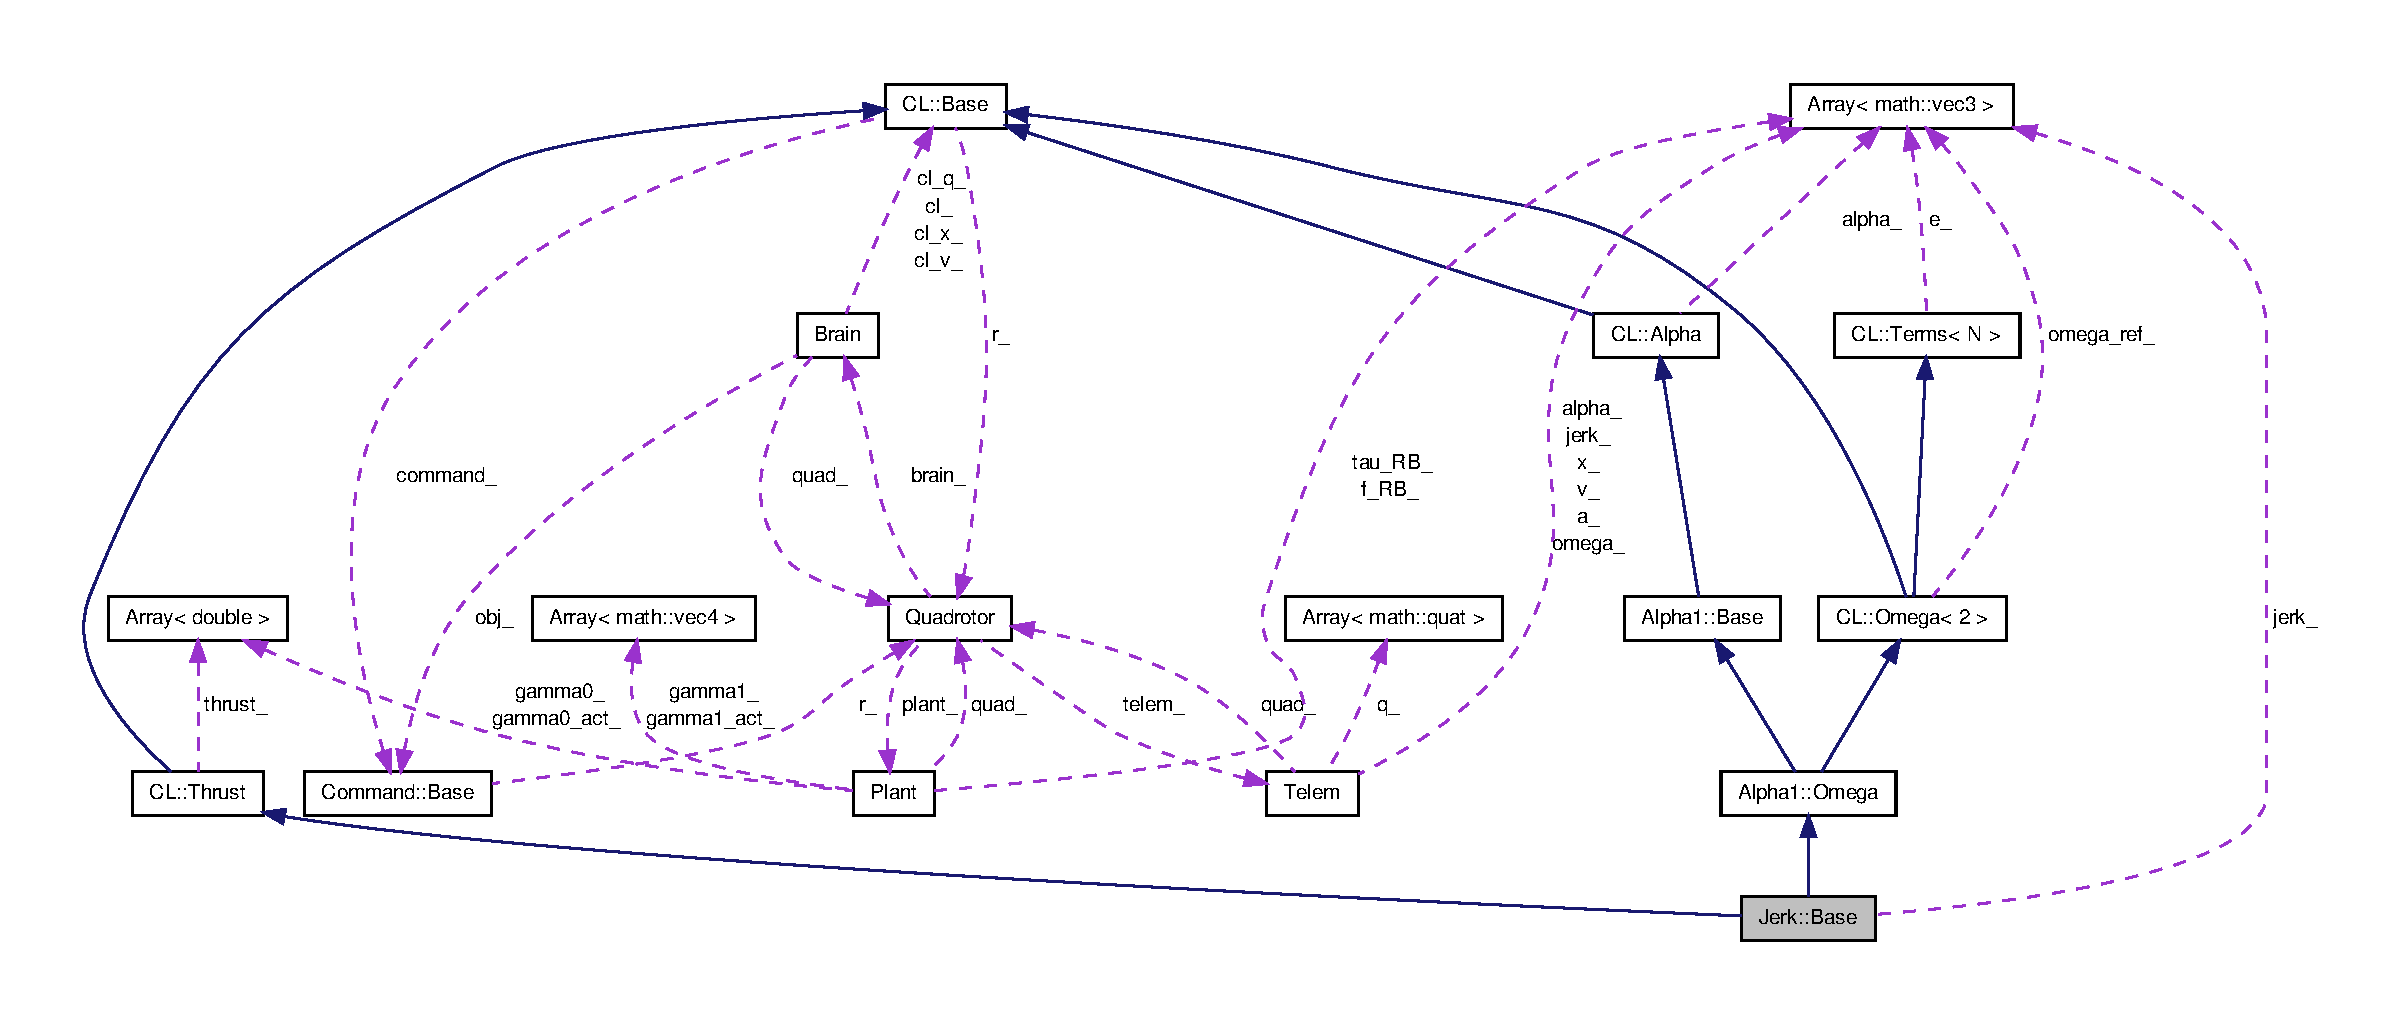
\includegraphics[width=350pt]{classJerk_1_1Base__coll__graph}
\end{center}
\end{figure}
\subsection*{\-Public \-Member \-Functions}
\begin{DoxyCompactItemize}
\item 
\hypertarget{classJerk_1_1Base_a626934eaadb98821638f7e372a4d3268}{{\bfseries \-Base} (\hyperlink{classQuadrotor}{\-Quadrotor} $\ast$)}\label{classJerk_1_1Base_a626934eaadb98821638f7e372a4d3268}

\item 
\hypertarget{classJerk_1_1Base_ac1207a2bf6d282ef432c072f99f57ef9}{virtual void {\bfseries \-Step} (int, double)=0}\label{classJerk_1_1Base_ac1207a2bf6d282ef432c072f99f57ef9}

\item 
\hypertarget{classJerk_1_1Base_aaa5aed35c31b51ef88dfcf82dc5c5f19}{virtual void {\bfseries alloc} (int)=0}\label{classJerk_1_1Base_aaa5aed35c31b51ef88dfcf82dc5c5f19}

\item 
\hypertarget{classJerk_1_1Base_ada482e98d0fe0542ce063a7413100f8f}{virtual void {\bfseries write} (int)}\label{classJerk_1_1Base_ada482e98d0fe0542ce063a7413100f8f}

\end{DoxyCompactItemize}
\subsection*{\-Public \-Attributes}
\begin{DoxyCompactItemize}
\item 
\hypertarget{classJerk_1_1Base_ae888b2ce4264998d26bb0bbfce51b5e7}{\hyperlink{classArray}{\-Array}$<$ math\-::vec3 $>$ {\bfseries jerk\-\_\-}}\label{classJerk_1_1Base_ae888b2ce4264998d26bb0bbfce51b5e7}

\end{DoxyCompactItemize}


\-The documentation for this class was generated from the following files\-:\begin{DoxyCompactItemize}
\item 
src/quadrotor/\-Control\-Law/\-Jerk.\-h\item 
src/quadrotor/\-Control\-Law/\-Jerk.\-cpp\end{DoxyCompactItemize}

\hypertarget{classJounce_1_1Base}{
\section{Jounce::Base Class Reference}
\label{classJounce_1_1Base}\index{Jounce::Base@{Jounce::Base}}
}
Inheritance diagram for Jounce::Base:Collaboration diagram for Jounce::Base:\subsection*{Public Member Functions}
\begin{DoxyCompactItemize}
\item 
\hypertarget{classJounce_1_1Base_a8e926179f18af0343dc9d155281a3fef}{
{\bfseries Base} (\hyperlink{classQuadrotor}{Quadrotor} $\ast$)}
\label{classJounce_1_1Base_a8e926179f18af0343dc9d155281a3fef}

\item 
\hypertarget{classJounce_1_1Base_ab541df0d26f27f1ed36584b0d44d3b36}{
virtual void {\bfseries Step} (int, double)=0}
\label{classJounce_1_1Base_ab541df0d26f27f1ed36584b0d44d3b36}

\item 
\hypertarget{classJounce_1_1Base_aba9478612b6891ea4fed47d15d2f0db8}{
virtual bool {\bfseries Check} (int, math::vec3)=0}
\label{classJounce_1_1Base_aba9478612b6891ea4fed47d15d2f0db8}

\item 
\hypertarget{classJounce_1_1Base_a83e3ef78e81ff6f85c46cda167a35cfa}{
virtual void {\bfseries alloc} (int)}
\label{classJounce_1_1Base_a83e3ef78e81ff6f85c46cda167a35cfa}

\item 
\hypertarget{classJounce_1_1Base_afd1ad723f86beb0fde0e960b835a958a}{
virtual void {\bfseries write} (int)}
\label{classJounce_1_1Base_afd1ad723f86beb0fde0e960b835a958a}

\end{DoxyCompactItemize}
\subsection*{Public Attributes}
\begin{DoxyCompactItemize}
\item 
\hypertarget{classJounce_1_1Base_ae4a19256fe64afbceb80c2fdbe584404}{
\hyperlink{classArray}{Array}$<$ math::vec3 $>$ {\bfseries jounce\_\-}}
\label{classJounce_1_1Base_ae4a19256fe64afbceb80c2fdbe584404}

\end{DoxyCompactItemize}


The documentation for this class was generated from the following files:\begin{DoxyCompactItemize}
\item 
src/quadrotor/ControlLaw/Jounce.h\item 
src/quadrotor/ControlLaw/Jounce.cpp\end{DoxyCompactItemize}

\hypertarget{classAlpha1_1_1Base}{\section{\-Alpha1\-:\-:\-Base \-Class \-Reference}
\label{classAlpha1_1_1Base}\index{\-Alpha1\-::\-Base@{\-Alpha1\-::\-Base}}
}


\-Inheritance diagram for \-Alpha1\-:\-:\-Base\-:\nopagebreak
\begin{figure}[H]
\begin{center}
\leavevmode
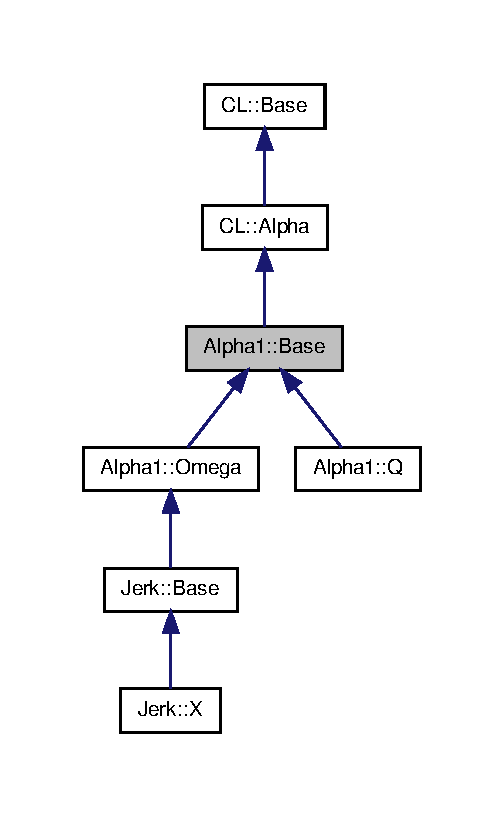
\includegraphics[width=242pt]{classAlpha1_1_1Base__inherit__graph}
\end{center}
\end{figure}


\-Collaboration diagram for \-Alpha1\-:\-:\-Base\-:\nopagebreak
\begin{figure}[H]
\begin{center}
\leavevmode
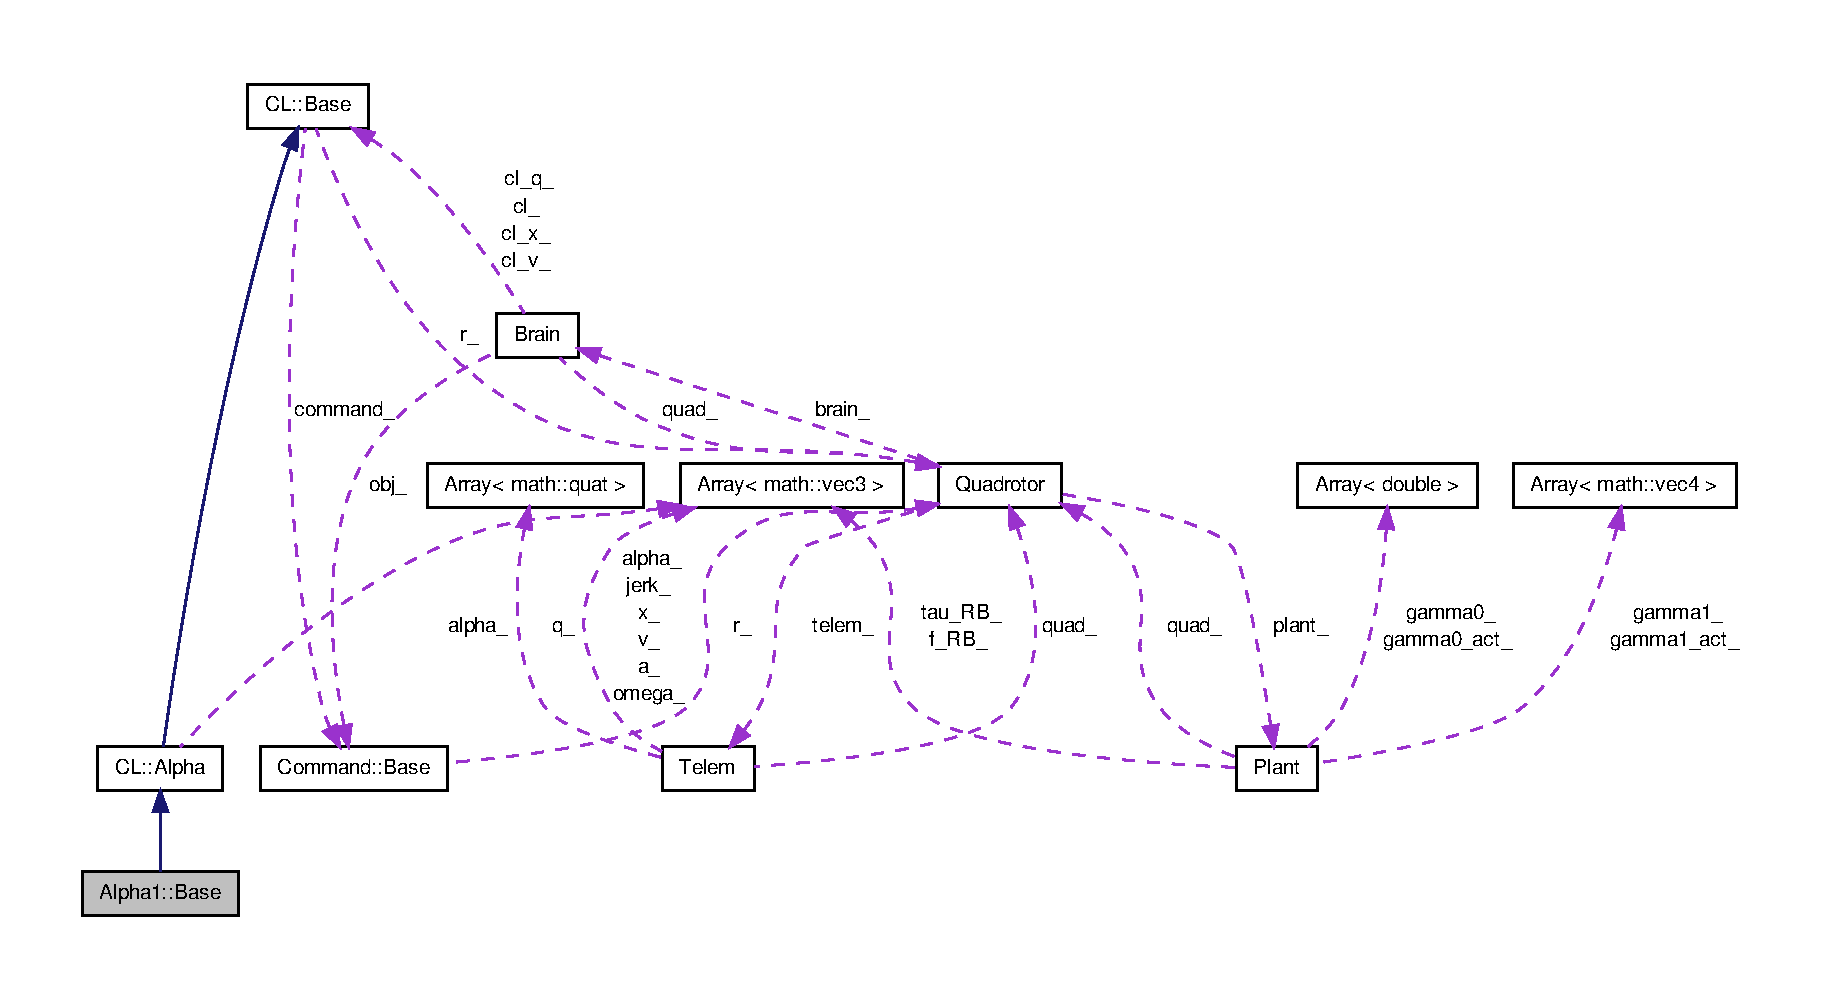
\includegraphics[width=350pt]{classAlpha1_1_1Base__coll__graph}
\end{center}
\end{figure}
\subsection*{\-Public \-Member \-Functions}
\begin{DoxyCompactItemize}
\item 
\hypertarget{classAlpha1_1_1Base_aa3a30d6a7eb5a05d313a17c3aadfbc46}{{\bfseries \-Base} (\hyperlink{classQuadrotor}{\-Quadrotor} $\ast$)}\label{classAlpha1_1_1Base_aa3a30d6a7eb5a05d313a17c3aadfbc46}

\item 
\hypertarget{classAlpha1_1_1Base_a8b2ac7103a87426eca6243d7e00a62a4}{void {\bfseries \-Step} (int i, double h)=0}\label{classAlpha1_1_1Base_a8b2ac7103a87426eca6243d7e00a62a4}

\item 
\hypertarget{classAlpha1_1_1Base_a760efb3a3d35444c4eaa465f9d39fd0f}{bool {\bfseries \-Check} (int, math\-::vec3)=0}\label{classAlpha1_1_1Base_a760efb3a3d35444c4eaa465f9d39fd0f}

\item 
\hypertarget{classAlpha1_1_1Base_a73c402f3bcb3d5b1cd97f867bd47a847}{virtual void {\bfseries write} (int)=0}\label{classAlpha1_1_1Base_a73c402f3bcb3d5b1cd97f867bd47a847}

\item 
\hypertarget{classAlpha1_1_1Base_a7039181204826d9000f98f3acc59938f}{virtual void {\bfseries alloc} (int)}\label{classAlpha1_1_1Base_a7039181204826d9000f98f3acc59938f}

\end{DoxyCompactItemize}


\-The documentation for this class was generated from the following files\-:\begin{DoxyCompactItemize}
\item 
src/quadrotor/\-Control\-Law/\-Alpha.\-h\item 
src/quadrotor/\-Control\-Law/\-Alpha.\-cpp\end{DoxyCompactItemize}

\hypertarget{classInput_1_1Vec3_1_1Base}{\section{\-Input\-:\-:\-Vec3\-:\-:\-Base \-Class \-Reference}
\label{classInput_1_1Vec3_1_1Base}\index{\-Input\-::\-Vec3\-::\-Base@{\-Input\-::\-Vec3\-::\-Base}}
}


\-Inheritance diagram for \-Input\-:\-:\-Vec3\-:\-:\-Base\-:\nopagebreak
\begin{figure}[H]
\begin{center}
\leavevmode
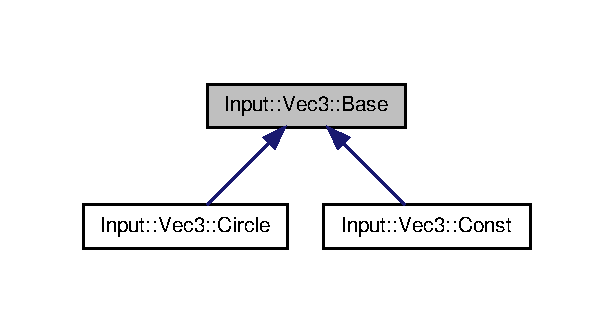
\includegraphics[width=294pt]{classInput_1_1Vec3_1_1Base__inherit__graph}
\end{center}
\end{figure}
\subsection*{\-Public \-Member \-Functions}
\begin{DoxyCompactItemize}
\item 
\hypertarget{classInput_1_1Vec3_1_1Base_a2cabb8020f12e27257a220e89136e2cd}{virtual math\-::vec3 {\bfseries f} (double)=0}\label{classInput_1_1Vec3_1_1Base_a2cabb8020f12e27257a220e89136e2cd}

\end{DoxyCompactItemize}


\-The documentation for this class was generated from the following file\-:\begin{DoxyCompactItemize}
\item 
src/quadrotor/\-Input.\-hpp\end{DoxyCompactItemize}

\hypertarget{classCL_1_1Base}{
\section{CL::Base Class Reference}
\label{classCL_1_1Base}\index{CL::Base@{CL::Base}}
}
Inheritance diagram for CL::Base:Collaboration diagram for CL::Base:\subsection*{Public Member Functions}
\begin{DoxyCompactItemize}
\item 
\hypertarget{classCL_1_1Base_ad8db38f548637316213cd109aed97792}{
{\bfseries Base} (\hyperlink{classQuadrotor}{Quadrotor} $\ast$r)}
\label{classCL_1_1Base_ad8db38f548637316213cd109aed97792}

\item 
\hypertarget{classCL_1_1Base_a08bb880fc7c5f5c81ee77eaa9570c32a}{
virtual void {\bfseries Step} (int, double)=0}
\label{classCL_1_1Base_a08bb880fc7c5f5c81ee77eaa9570c32a}

\item 
\hypertarget{classCL_1_1Base_a3de68eff20bc897fea32c758bff81d03}{
virtual bool {\bfseries Check} (int, math::vec3)=0}
\label{classCL_1_1Base_a3de68eff20bc897fea32c758bff81d03}

\item 
\hypertarget{classCL_1_1Base_ab4f3f33c7eb3869ca36490255600c3a5}{
virtual void {\bfseries alloc} (int)=0}
\label{classCL_1_1Base_ab4f3f33c7eb3869ca36490255600c3a5}

\item 
\hypertarget{classCL_1_1Base_ab23d401d25f004ee0e7ef20a591a6ba2}{
virtual void {\bfseries write} (int)=0}
\label{classCL_1_1Base_ab23d401d25f004ee0e7ef20a591a6ba2}

\item 
\hypertarget{classCL_1_1Base_acbc68636ede90524743ffb85dd41aa0c}{
virtual void {\bfseries Init} (int)}
\label{classCL_1_1Base_acbc68636ede90524743ffb85dd41aa0c}

\end{DoxyCompactItemize}
\subsection*{Public Attributes}
\begin{DoxyCompactItemize}
\item 
\hypertarget{classCL_1_1Base_ad96040f9fcd19572e9e73dbafc62f801}{
\hyperlink{classQuadrotor}{Quadrotor} $\ast$ {\bfseries r\_\-}}
\label{classCL_1_1Base_ad96040f9fcd19572e9e73dbafc62f801}

\item 
\hypertarget{classCL_1_1Base_aacd59a4cfd28c0bb1fbb468193cf8780}{
\hyperlink{classCommand_1_1Base}{Command::Base} $\ast$ {\bfseries command\_\-}}
\label{classCL_1_1Base_aacd59a4cfd28c0bb1fbb468193cf8780}

\end{DoxyCompactItemize}


The documentation for this class was generated from the following files:\begin{DoxyCompactItemize}
\item 
src/quadrotor/ControlLaw/ControlLaw.h\item 
src/quadrotor/ControlLaw/ControlLaw.cpp\end{DoxyCompactItemize}

\hypertarget{classCommand_1_1Base}{
\section{Command::Base Class Reference}
\label{classCommand_1_1Base}\index{Command::Base@{Command::Base}}
}
Inheritance diagram for Command::Base:Collaboration diagram for Command::Base:\subsection*{Classes}
\begin{DoxyCompactItemize}
\item 
struct \hyperlink{structCommand_1_1Base_1_1Flag}{Flag}
\item 
struct \hyperlink{structCommand_1_1Base_1_1Type}{Type}
\end{DoxyCompactItemize}
\subsection*{Public Member Functions}
\begin{DoxyCompactItemize}
\item 
\hypertarget{classCommand_1_1Base_acfdd5eee18d39adfcbe321970d4f27fc}{
{\bfseries Base} (\hyperlink{classQuadrotor}{Quadrotor} $\ast$, Type::e)}
\label{classCommand_1_1Base_acfdd5eee18d39adfcbe321970d4f27fc}

\item 
\hypertarget{classCommand_1_1Base_a1a77b2acc5e0a41d1eee5ab61c2dfafd}{
virtual void {\bfseries Check} (int)}
\label{classCommand_1_1Base_a1a77b2acc5e0a41d1eee5ab61c2dfafd}

\item 
\hypertarget{classCommand_1_1Base_ab85e28c51f1601c05532d68b9a71f425}{
virtual void {\bfseries Start} (int)}
\label{classCommand_1_1Base_ab85e28c51f1601c05532d68b9a71f425}

\end{DoxyCompactItemize}
\subsection*{Public Attributes}
\begin{DoxyCompactItemize}
\item 
\hypertarget{classCommand_1_1Base_ad10b11ae9f939a0d88eec17591389106}{
\hyperlink{classQuadrotor}{Quadrotor} $\ast$ {\bfseries r\_\-}}
\label{classCommand_1_1Base_ad10b11ae9f939a0d88eec17591389106}

\item 
\hypertarget{classCommand_1_1Base_af73a59e7026b8f879d7bc4a8091b729c}{
unsigned int {\bfseries flag\_\-}}
\label{classCommand_1_1Base_af73a59e7026b8f879d7bc4a8091b729c}

\item 
\hypertarget{classCommand_1_1Base_a9f27c385185e92121075275d2d9b8eba}{
unsigned int {\bfseries mode\_\-}}
\label{classCommand_1_1Base_a9f27c385185e92121075275d2d9b8eba}

\item 
\hypertarget{classCommand_1_1Base_acb491ef2bb4053594e77e877aaecfade}{
unsigned int {\bfseries type\_\-}}
\label{classCommand_1_1Base_acb491ef2bb4053594e77e877aaecfade}

\item 
\hypertarget{classCommand_1_1Base_ae8f49ff59722fb70fcf4d735129ef23a}{
std::vector$<$ \hyperlink{classCommand_1_1Stop_1_1Base}{Command::Stop::Base} $\ast$ $>$ {\bfseries stop\_\-}}
\label{classCommand_1_1Base_ae8f49ff59722fb70fcf4d735129ef23a}

\end{DoxyCompactItemize}


The documentation for this class was generated from the following files:\begin{DoxyCompactItemize}
\item 
src/quadrotor/command.h\item 
src/quadrotor/command.cpp\end{DoxyCompactItemize}

\hypertarget{classCommand_1_1Stop_1_1Base}{
\section{Command::Stop::Base Class Reference}
\label{classCommand_1_1Stop_1_1Base}\index{Command::Stop::Base@{Command::Stop::Base}}
}
Inheritance diagram for Command::Stop::Base:Collaboration diagram for Command::Stop::Base:\subsection*{Public Member Functions}
\begin{DoxyCompactItemize}
\item 
\hypertarget{classCommand_1_1Stop_1_1Base_a5aad1b25a4bef2187a1901c1522b3fc6}{
{\bfseries Base} (\hyperlink{classCommand_1_1Base}{Command::Base} $\ast$cmd)}
\label{classCommand_1_1Stop_1_1Base_a5aad1b25a4bef2187a1901c1522b3fc6}

\item 
\hypertarget{classCommand_1_1Stop_1_1Base_a9b64cdd96ab19d1821d97fc6a4d58071}{
virtual void {\bfseries Check} (int)=0}
\label{classCommand_1_1Stop_1_1Base_a9b64cdd96ab19d1821d97fc6a4d58071}

\end{DoxyCompactItemize}
\subsection*{Public Attributes}
\begin{DoxyCompactItemize}
\item 
\hypertarget{classCommand_1_1Stop_1_1Base_a76255ee63c35b52931e8dfc12a4adb3f}{
\begin{tabbing}
xx\=xx\=xx\=xx\=xx\=xx\=xx\=xx\=xx\=\kill
struct \{\\
\>double {\bfseries t\_}\\
\>int {\bfseries i\_}\\
\} {\bfseries stats\_}}
\label{classCommand_1_1Stop_1_1Base_a76255ee63c35b52931e8dfc12a4adb3f}
\\

\end{tabbing}\item 
\hypertarget{classCommand_1_1Stop_1_1Base_a6dc4d26ec6c6fb985e0c5bc649f67870}{
\hyperlink{classCommand_1_1Base}{Command::Base} $\ast$ {\bfseries cmd\_\-}}
\label{classCommand_1_1Stop_1_1Base_a6dc4d26ec6c6fb985e0c5bc649f67870}

\end{DoxyCompactItemize}


The documentation for this class was generated from the following file:\begin{DoxyCompactItemize}
\item 
src/quadrotor/command/Stop.hpp\end{DoxyCompactItemize}

\hypertarget{classBrain}{
\section{Brain Class Reference}
\label{classBrain}\index{Brain@{Brain}}
}
Collaboration diagram for Brain:\subsection*{Classes}
\begin{DoxyCompactItemize}
\item 
struct \hyperlink{structBrain_1_1Mode}{Mode}
\end{DoxyCompactItemize}
\subsection*{Public Member Functions}
\begin{DoxyCompactItemize}
\item 
\hypertarget{classBrain_ad661eb184de49991281a1913d71dbad5}{
{\bfseries Brain} (\hyperlink{classQuadrotor}{Quadrotor} $\ast$)}
\label{classBrain_ad661eb184de49991281a1913d71dbad5}

\item 
\hypertarget{classBrain_ab45d9d639fdf6fa9f7d24e3f4272d35f}{
void {\bfseries reset} ()}
\label{classBrain_ab45d9d639fdf6fa9f7d24e3f4272d35f}

\item 
\hypertarget{classBrain_af0033e0a76b1dbab2935ca93b1008dad}{
void {\bfseries CheckCommand} (int)}
\label{classBrain_af0033e0a76b1dbab2935ca93b1008dad}

\item 
\hypertarget{classBrain_a7f03601463650611a436793da2b80abd}{
void {\bfseries step} (int ti, double dt)}
\label{classBrain_a7f03601463650611a436793da2b80abd}

\item 
\hypertarget{classBrain_a3117d293a1087e00f2ba05cf3099a0ae}{
void {\bfseries write} (int ti)}
\label{classBrain_a3117d293a1087e00f2ba05cf3099a0ae}

\end{DoxyCompactItemize}
\subsection*{Public Attributes}
\begin{DoxyCompactItemize}
\item 
\hypertarget{classBrain_a909cbf59a243e11be1e052dfebc1039f}{
int {\bfseries mode\_\-}}
\label{classBrain_a909cbf59a243e11be1e052dfebc1039f}

\item 
\hypertarget{classBrain_a522cd8559636661c43d07aa86e9803b7}{
\hyperlink{classQuadrotor}{Quadrotor} $\ast$ {\bfseries quad\_\-}}
\label{classBrain_a522cd8559636661c43d07aa86e9803b7}

\item 
\hypertarget{classBrain_a0897765690afb51c87d037329e968464}{
\hyperlink{classCL_1_1Base}{CL::Base} $\ast$ {\bfseries cl\_\-}}
\label{classBrain_a0897765690afb51c87d037329e968464}

\item 
\hypertarget{classBrain_aa408572807d4347bd4a7e3bee61ee75e}{
\hyperlink{classCL_1_1Base}{CL::Base} $\ast$ {\bfseries cl\_\-x\_\-}}
\label{classBrain_aa408572807d4347bd4a7e3bee61ee75e}

\item 
\hypertarget{classBrain_af283fe2f0a5ee9cb117cc393a0028993}{
\hyperlink{classCL_1_1Base}{CL::Base} $\ast$ {\bfseries cl\_\-v\_\-}}
\label{classBrain_af283fe2f0a5ee9cb117cc393a0028993}

\item 
\hypertarget{classBrain_a962d23b524a3bf3668eb3f6bdf5be20e}{
\hyperlink{classCL_1_1Base}{CL::Base} $\ast$ {\bfseries cl\_\-q\_\-}}
\label{classBrain_a962d23b524a3bf3668eb3f6bdf5be20e}

\item 
\hypertarget{classBrain_a839638574da324a41c61edd5375a7261}{
double {\bfseries heading\_\-}}
\label{classBrain_a839638574da324a41c61edd5375a7261}

\item 
\hypertarget{classBrain_a9e99f325288e528a5893ff37dce19ec7}{
std::deque$<$ \hyperlink{classCommand_1_1Base}{Command::Base} $\ast$ $>$ {\bfseries objs\_\-}}
\label{classBrain_a9e99f325288e528a5893ff37dce19ec7}

\item 
\hypertarget{classBrain_add3bf09bdcdd4cfc8008d076b1859f5f}{
\hyperlink{classCommand_1_1Base}{Command::Base} $\ast$ {\bfseries obj\_\-}}
\label{classBrain_add3bf09bdcdd4cfc8008d076b1859f5f}

\end{DoxyCompactItemize}


The documentation for this class was generated from the following files:\begin{DoxyCompactItemize}
\item 
src/quadrotor/brain.h\item 
src/quadrotor/brain.cpp\end{DoxyCompactItemize}

\hypertarget{classInput_1_1Vec3_1_1Circle}{\section{\-Input\-:\-:\-Vec3\-:\-:\-Circle \-Class \-Reference}
\label{classInput_1_1Vec3_1_1Circle}\index{\-Input\-::\-Vec3\-::\-Circle@{\-Input\-::\-Vec3\-::\-Circle}}
}


\-Inheritance diagram for \-Input\-:\-:\-Vec3\-:\-:\-Circle\-:\nopagebreak
\begin{figure}[H]
\begin{center}
\leavevmode
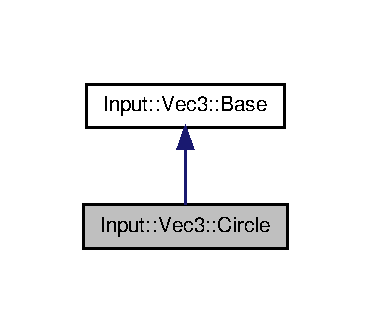
\includegraphics[width=178pt]{classInput_1_1Vec3_1_1Circle__inherit__graph}
\end{center}
\end{figure}


\-Collaboration diagram for \-Input\-:\-:\-Vec3\-:\-:\-Circle\-:\nopagebreak
\begin{figure}[H]
\begin{center}
\leavevmode
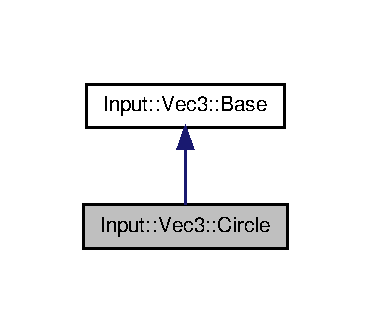
\includegraphics[width=178pt]{classInput_1_1Vec3_1_1Circle__coll__graph}
\end{center}
\end{figure}
\subsection*{\-Public \-Member \-Functions}
\begin{DoxyCompactItemize}
\item 
\hypertarget{classInput_1_1Vec3_1_1Circle_a37e8e683d26d784fa1cc05934f660384}{{\bfseries \-Circle} (double r, double \-T)}\label{classInput_1_1Vec3_1_1Circle_a37e8e683d26d784fa1cc05934f660384}

\item 
\hypertarget{classInput_1_1Vec3_1_1Circle_a8a20d13a80afea6b50d200acf9fcf956}{virtual math\-::vec3 {\bfseries f} (double t)}\label{classInput_1_1Vec3_1_1Circle_a8a20d13a80afea6b50d200acf9fcf956}

\end{DoxyCompactItemize}
\subsection*{\-Public \-Attributes}
\begin{DoxyCompactItemize}
\item 
\hypertarget{classInput_1_1Vec3_1_1Circle_a49ae5e8e06e3bfa8c66c98e13d89f706}{double {\bfseries r\-\_\-}}\label{classInput_1_1Vec3_1_1Circle_a49ae5e8e06e3bfa8c66c98e13d89f706}

\item 
\hypertarget{classInput_1_1Vec3_1_1Circle_a873c9bcd953193a827cfa9e92ea1740a}{double {\bfseries \-T\-\_\-}}\label{classInput_1_1Vec3_1_1Circle_a873c9bcd953193a827cfa9e92ea1740a}

\item 
\hypertarget{classInput_1_1Vec3_1_1Circle_a3dc1f92e4adb3f85ed7073d25e287cbc}{double {\bfseries omega\-\_\-}}\label{classInput_1_1Vec3_1_1Circle_a3dc1f92e4adb3f85ed7073d25e287cbc}

\end{DoxyCompactItemize}


\-The documentation for this class was generated from the following file\-:\begin{DoxyCompactItemize}
\item 
src/quadrotor/\-Input.\-hpp\end{DoxyCompactItemize}

\hypertarget{classInput_1_1Vec3_1_1Const}{
\section{Input::Vec3::Const Class Reference}
\label{classInput_1_1Vec3_1_1Const}\index{Input::Vec3::Const@{Input::Vec3::Const}}
}
Inheritance diagram for Input::Vec3::Const:Collaboration diagram for Input::Vec3::Const:\subsection*{Public Member Functions}
\begin{DoxyCompactItemize}
\item 
\hypertarget{classInput_1_1Vec3_1_1Const_ac7ec7f1798a13524dac263d63660ee64}{
{\bfseries Const} (math::vec3 v)}
\label{classInput_1_1Vec3_1_1Const_ac7ec7f1798a13524dac263d63660ee64}

\item 
\hypertarget{classInput_1_1Vec3_1_1Const_ad2fdc41feb2afc22fbc7bda5fae71fba}{
virtual math::vec3 {\bfseries f} (double)}
\label{classInput_1_1Vec3_1_1Const_ad2fdc41feb2afc22fbc7bda5fae71fba}

\end{DoxyCompactItemize}
\subsection*{Public Attributes}
\begin{DoxyCompactItemize}
\item 
\hypertarget{classInput_1_1Vec3_1_1Const_a3fa537d473ff297a1581031e0ba593b4}{
math::vec3 {\bfseries v\_\-}}
\label{classInput_1_1Vec3_1_1Const_a3fa537d473ff297a1581031e0ba593b4}

\end{DoxyCompactItemize}


The documentation for this class was generated from the following file:\begin{DoxyCompactItemize}
\item 
src/quadrotor/Input.hpp\end{DoxyCompactItemize}

\hypertarget{classEmptyQueue}{
\section{EmptyQueue Class Reference}
\label{classEmptyQueue}\index{EmptyQueue@{EmptyQueue}}
}
Inheritance diagram for EmptyQueue:Collaboration diagram for EmptyQueue:\subsection*{Public Member Functions}
\begin{DoxyCompactItemize}
\item 
\hypertarget{classEmptyQueue_a57d73966a7700462d877b441299522d0}{
virtual const char $\ast$ {\bfseries what} () const   throw ()}
\label{classEmptyQueue_a57d73966a7700462d877b441299522d0}

\end{DoxyCompactItemize}


The documentation for this class was generated from the following file:\begin{DoxyCompactItemize}
\item 
src/quadrotor/except.h\end{DoxyCompactItemize}

\hypertarget{structCommand_1_1Base_1_1Flag}{\section{\-Command\-:\-:\-Base\-:\-:\-Flag \-Struct \-Reference}
\label{structCommand_1_1Base_1_1Flag}\index{\-Command\-::\-Base\-::\-Flag@{\-Command\-::\-Base\-::\-Flag}}
}
\subsection*{\-Public \-Types}
\begin{DoxyCompactItemize}
\item 
enum {\bfseries e} \{ {\bfseries \-R\-I\-S\-E} =  1 $<$$<$ 0, 
{\bfseries \-S\-E\-T\-T\-L\-E} =  1 $<$$<$ 1, 
{\bfseries \-C\-O\-M\-P\-L\-E\-T\-E} =  1 $<$$<$ 2
 \}
\end{DoxyCompactItemize}


\-The documentation for this struct was generated from the following file\-:\begin{DoxyCompactItemize}
\item 
src/quadrotor/command.\-h\end{DoxyCompactItemize}

\hypertarget{classCommand_1_1Freeze}{
\section{Command::Freeze Class Reference}
\label{classCommand_1_1Freeze}\index{Command::Freeze@{Command::Freeze}}
}
Inheritance diagram for Command::Freeze:Collaboration diagram for Command::Freeze:\subsection*{Public Member Functions}
\begin{DoxyCompactItemize}
\item 
\hypertarget{classCommand_1_1Freeze_aec86b6e382bba9633b4eb7f965080265}{
{\bfseries Freeze} (\hyperlink{classQuadrotor}{Quadrotor} $\ast$r)}
\label{classCommand_1_1Freeze_aec86b6e382bba9633b4eb7f965080265}

\item 
\hypertarget{classCommand_1_1Freeze_a2903673ebb811dc5b18177d9b0ac174a}{
virtual void {\bfseries Start} (int)}
\label{classCommand_1_1Freeze_a2903673ebb811dc5b18177d9b0ac174a}

\end{DoxyCompactItemize}


The documentation for this class was generated from the following files:\begin{DoxyCompactItemize}
\item 
src/quadrotor/command.h\item 
src/quadrotor/command.cpp\end{DoxyCompactItemize}

\hypertarget{classInf}{
\section{Inf Class Reference}
\label{classInf}\index{Inf@{Inf}}
}
Inheritance diagram for Inf:Collaboration diagram for Inf:\subsection*{Public Member Functions}
\begin{DoxyCompactItemize}
\item 
\hypertarget{classInf_ad631c9e417358223b219a0d27321ccab}{
virtual const char $\ast$ {\bfseries what} () const   throw ()}
\label{classInf_ad631c9e417358223b219a0d27321ccab}

\end{DoxyCompactItemize}


The documentation for this class was generated from the following file:\begin{DoxyCompactItemize}
\item 
src/quadrotor/except.h\end{DoxyCompactItemize}

\hypertarget{classInvalidOp}{\section{\-Invalid\-Op \-Class \-Reference}
\label{classInvalidOp}\index{\-Invalid\-Op@{\-Invalid\-Op}}
}


\-Inheritance diagram for \-Invalid\-Op\-:\nopagebreak
\begin{figure}[H]
\begin{center}
\leavevmode
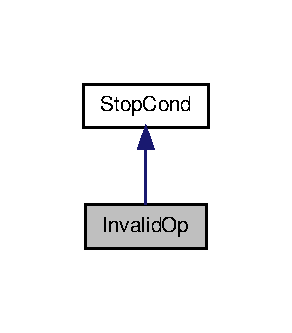
\includegraphics[width=140pt]{classInvalidOp__inherit__graph}
\end{center}
\end{figure}


\-Collaboration diagram for \-Invalid\-Op\-:\nopagebreak
\begin{figure}[H]
\begin{center}
\leavevmode
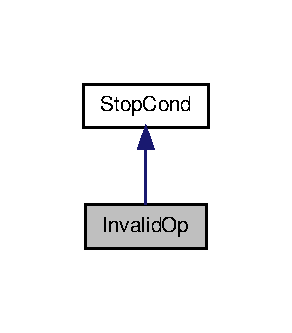
\includegraphics[width=140pt]{classInvalidOp__coll__graph}
\end{center}
\end{figure}
\subsection*{\-Public \-Member \-Functions}
\begin{DoxyCompactItemize}
\item 
\hypertarget{classInvalidOp_ad89cda4b62702beb435e982f0c8b9e42}{virtual const char $\ast$ {\bfseries what} () const   throw ()}\label{classInvalidOp_ad89cda4b62702beb435e982f0c8b9e42}

\end{DoxyCompactItemize}


\-The documentation for this class was generated from the following file\-:\begin{DoxyCompactItemize}
\item 
src/quadrotor/except.\-h\end{DoxyCompactItemize}

\hypertarget{structBrain_1_1Mode}{\section{\-Brain\-:\-:\-Mode \-Struct \-Reference}
\label{structBrain_1_1Mode}\index{\-Brain\-::\-Mode@{\-Brain\-::\-Mode}}
}
\subsection*{\-Public \-Types}
\begin{DoxyCompactItemize}
\item 
enum {\bfseries e} \{ {\bfseries \-N\-O\-N\-E} =  0, 
{\bfseries \-A\-C\-C\-E\-L}, 
{\bfseries \-J\-E\-R\-K}, 
{\bfseries \-J\-O\-U\-N\-C\-E}
 \}
\end{DoxyCompactItemize}


\-The documentation for this struct was generated from the following file\-:\begin{DoxyCompactItemize}
\item 
src/quadrotor/brain.\-h\end{DoxyCompactItemize}

\hypertarget{structAttitude_1_1Mode}{\section{\-Attitude\-:\-:\-Mode \-Struct \-Reference}
\label{structAttitude_1_1Mode}\index{\-Attitude\-::\-Mode@{\-Attitude\-::\-Mode}}
}
\subsection*{\-Public \-Types}
\begin{DoxyCompactItemize}
\item 
enum {\bfseries e} \{ {\bfseries \-A\-T\-T}, 
{\bfseries \-V\-E\-L}, 
{\bfseries \-N\-O\-N\-E}
 \}
\end{DoxyCompactItemize}


\-The documentation for this struct was generated from the following file\-:\begin{DoxyCompactItemize}
\item 
src/quadrotor/attitude.\-h\end{DoxyCompactItemize}

\hypertarget{classAlpha1_1_1Omega}{
\section{Alpha1::Omega Class Reference}
\label{classAlpha1_1_1Omega}\index{Alpha1::Omega@{Alpha1::Omega}}
}
Inheritance diagram for Alpha1::Omega:Collaboration diagram for Alpha1::Omega:\subsection*{Public Member Functions}
\begin{DoxyCompactItemize}
\item 
\hypertarget{classAlpha1_1_1Omega_a32a0b92a692f2e8aeecab24d5679bfaf}{
{\bfseries Omega} (\hyperlink{classQuadrotor}{Quadrotor} $\ast$r)}
\label{classAlpha1_1_1Omega_a32a0b92a692f2e8aeecab24d5679bfaf}

\item 
\hypertarget{classAlpha1_1_1Omega_ad5ee7dce47604f655179fa60a262e993}{
void {\bfseries Step} (int i, double h)}
\label{classAlpha1_1_1Omega_ad5ee7dce47604f655179fa60a262e993}

\item 
\hypertarget{classAlpha1_1_1Omega_a1e6326c0e02fa47343c92e22adaa37c1}{
bool {\bfseries Check} (int, math::vec3)}
\label{classAlpha1_1_1Omega_a1e6326c0e02fa47343c92e22adaa37c1}

\item 
\hypertarget{classAlpha1_1_1Omega_a43530dec2383d0dc669faf55f4d3aab8}{
virtual void {\bfseries write} (int)}
\label{classAlpha1_1_1Omega_a43530dec2383d0dc669faf55f4d3aab8}

\item 
\hypertarget{classAlpha1_1_1Omega_ad24c9b64337b0a74c42675590664ed7c}{
virtual void {\bfseries alloc} (int)}
\label{classAlpha1_1_1Omega_ad24c9b64337b0a74c42675590664ed7c}

\end{DoxyCompactItemize}


The documentation for this class was generated from the following files:\begin{DoxyCompactItemize}
\item 
src/quadrotor/ControlLaw/Alpha.h\item 
src/quadrotor/ControlLaw/Alpha.cpp\end{DoxyCompactItemize}

\hypertarget{classCL_1_1Omega}{\section{\-C\-L\-:\-:\-Omega$<$ \-N $>$ \-Class \-Template \-Reference}
\label{classCL_1_1Omega}\index{\-C\-L\-::\-Omega$<$ N $>$@{\-C\-L\-::\-Omega$<$ N $>$}}
}


\-Inheritance diagram for \-C\-L\-:\-:\-Omega$<$ \-N $>$\-:\nopagebreak
\begin{figure}[H]
\begin{center}
\leavevmode
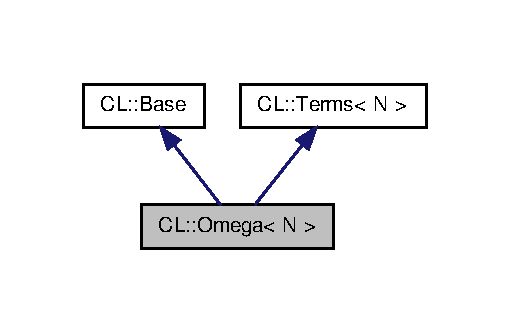
\includegraphics[width=244pt]{classCL_1_1Omega__inherit__graph}
\end{center}
\end{figure}


\-Collaboration diagram for \-C\-L\-:\-:\-Omega$<$ \-N $>$\-:\nopagebreak
\begin{figure}[H]
\begin{center}
\leavevmode
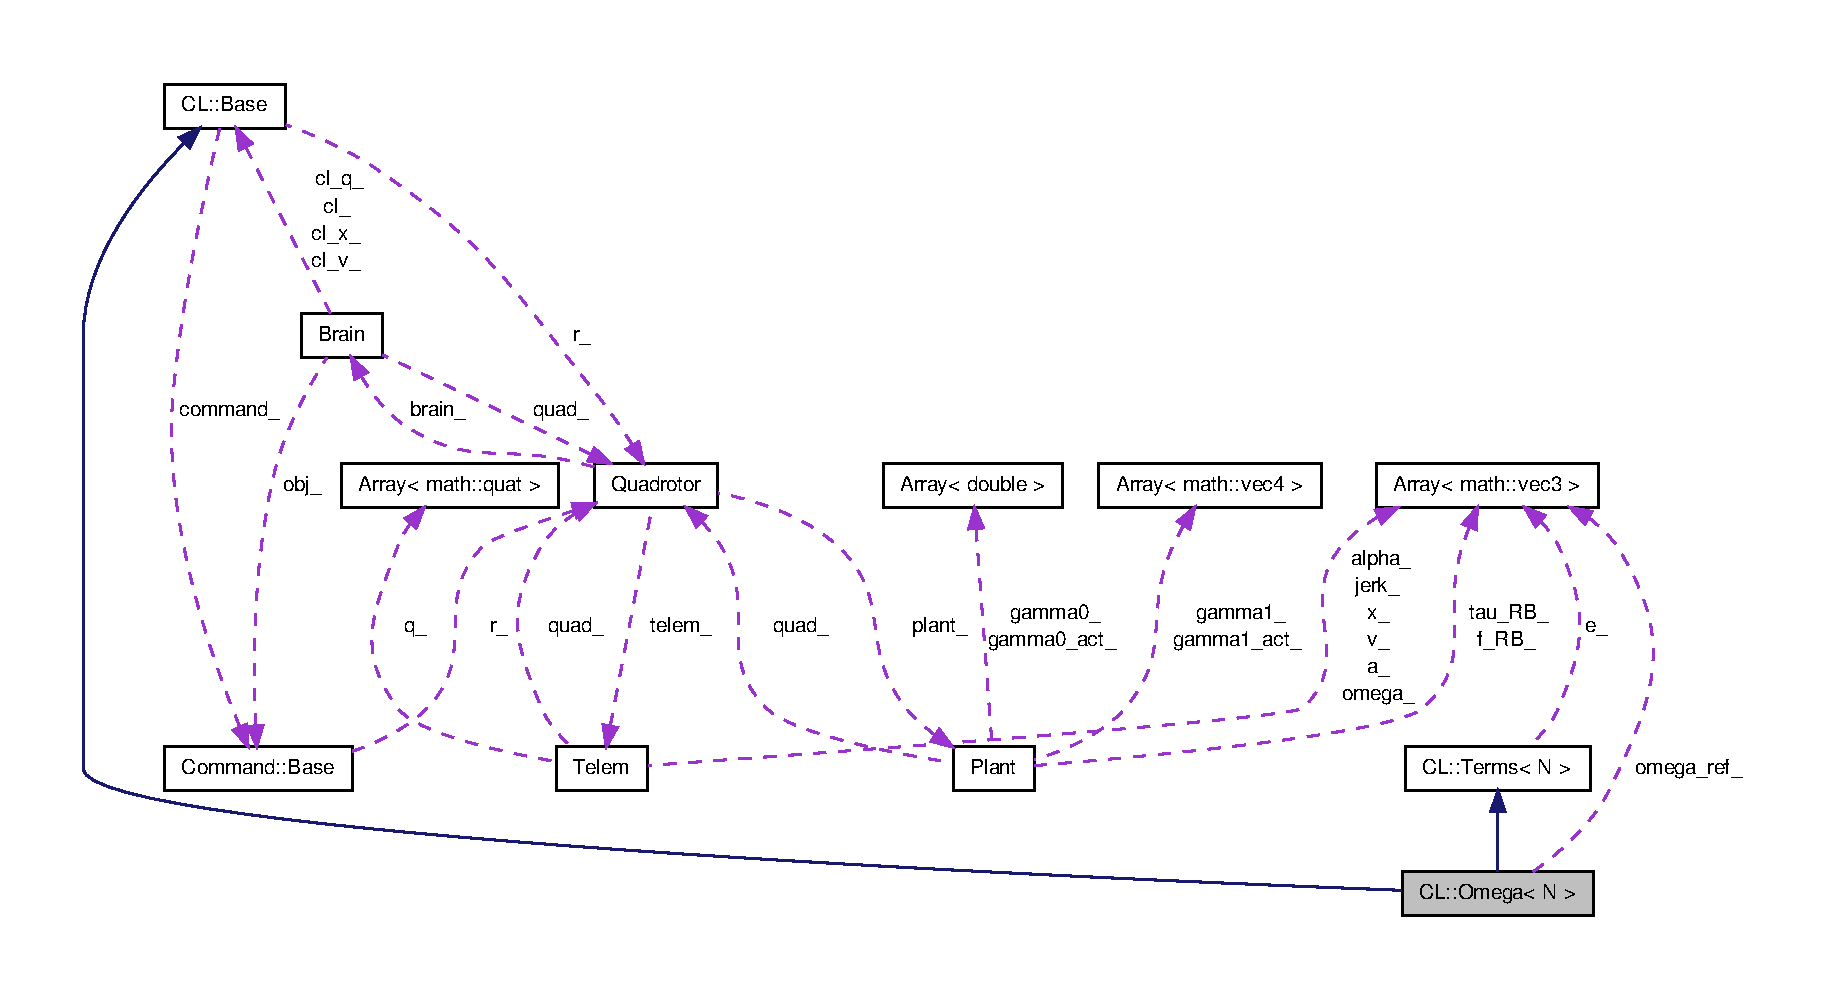
\includegraphics[width=350pt]{classCL_1_1Omega__coll__graph}
\end{center}
\end{figure}
\subsection*{\-Public \-Member \-Functions}
\begin{DoxyCompactItemize}
\item 
\hypertarget{classCL_1_1Omega_afcbb238467282d3addd88508937fe37c}{{\bfseries \-Omega} (\hyperlink{classQuadrotor}{\-Quadrotor} $\ast$r)}\label{classCL_1_1Omega_afcbb238467282d3addd88508937fe37c}

\item 
\hypertarget{classCL_1_1Omega_a68c53ed2e6669dec2f66517fcb42f92e}{virtual void {\bfseries alloc} (int n)}\label{classCL_1_1Omega_a68c53ed2e6669dec2f66517fcb42f92e}

\item 
\hypertarget{classCL_1_1Omega_ade07f74d9a84305b7be781911a1b0930}{virtual void {\bfseries write} (int n)}\label{classCL_1_1Omega_ade07f74d9a84305b7be781911a1b0930}

\end{DoxyCompactItemize}
\subsection*{\-Public \-Attributes}
\begin{DoxyCompactItemize}
\item 
\hypertarget{classCL_1_1Omega_afb1f31f1519495a3e0e9d3fe22b09bd0}{\hyperlink{classArray}{\-Array}$<$ math\-::vec3 $>$ {\bfseries omega\-\_\-ref\-\_\-} \mbox{[}2\mbox{]}}\label{classCL_1_1Omega_afb1f31f1519495a3e0e9d3fe22b09bd0}

\end{DoxyCompactItemize}
\subsubsection*{template$<$int \-N$>$ class C\-L\-::\-Omega$<$ N $>$}



\-The documentation for this class was generated from the following file\-:\begin{DoxyCompactItemize}
\item 
src/quadrotor/\-Control\-Law/\-Control\-Law.\-h\end{DoxyCompactItemize}

\hypertarget{classOmegaHigh}{
\section{OmegaHigh Class Reference}
\label{classOmegaHigh}\index{OmegaHigh@{OmegaHigh}}
}
Inheritance diagram for OmegaHigh:Collaboration diagram for OmegaHigh:\subsection*{Public Member Functions}
\begin{DoxyCompactItemize}
\item 
\hypertarget{classOmegaHigh_a9b61b9efec3c6adf95be4db650903c81}{
virtual const char $\ast$ {\bfseries what} () const   throw ()}
\label{classOmegaHigh_a9b61b9efec3c6adf95be4db650903c81}

\end{DoxyCompactItemize}


The documentation for this class was generated from the following file:\begin{DoxyCompactItemize}
\item 
src/quadrotor/except.h\end{DoxyCompactItemize}

\hypertarget{classPlant}{
\section{Plant Class Reference}
\label{classPlant}\index{Plant@{Plant}}
}
Collaboration diagram for Plant:\subsection*{Public Member Functions}
\begin{DoxyCompactItemize}
\item 
\hypertarget{classPlant_a142ca8e3ae860d3b93f5de973be71e39}{
{\bfseries Plant} (\hyperlink{classQuadrotor}{Quadrotor} $\ast$quad)}
\label{classPlant_a142ca8e3ae860d3b93f5de973be71e39}

\item 
\hypertarget{classPlant_a9b61938a3973f7dc3bd2511bcb377615}{
math::vec3 {\bfseries get\_\-tau\_\-body} (int ti)}
\label{classPlant_a9b61938a3973f7dc3bd2511bcb377615}

\item 
\hypertarget{classPlant_a0cd2196cba6ec3725c7d3c9146ae2f3c}{
void {\bfseries step\_\-rotor\_\-body} (int ti)}
\label{classPlant_a0cd2196cba6ec3725c7d3c9146ae2f3c}

\item 
\hypertarget{classPlant_a0aec8e6b4599646841cbf16370e8726c}{
math::vec3 {\bfseries get\_\-force\_\-rotor\_\-body} (int ti)}
\label{classPlant_a0aec8e6b4599646841cbf16370e8726c}

\item 
\hypertarget{classPlant_a103c83a20c439d3944f14fca3aa42cd1}{
math::vec3 {\bfseries get\_\-force\_\-drag\_\-body} (int ti)}
\label{classPlant_a103c83a20c439d3944f14fca3aa42cd1}

\item 
\hypertarget{classPlant_a5d36154e55ed37ade1997289fe6dbdf9}{
math::vec3 {\bfseries get\_\-force\_\-drag} (int ti)}
\label{classPlant_a5d36154e55ed37ade1997289fe6dbdf9}

\item 
\hypertarget{classPlant_a992691a9ab2614199f2295dc825d583b}{
math::vec3 {\bfseries get\_\-force} (int ti)}
\label{classPlant_a992691a9ab2614199f2295dc825d583b}

\item 
\hypertarget{classPlant_af5c6f03354c0cf11a968e88381fe89ab}{
void {\bfseries step} (int ti)}
\label{classPlant_af5c6f03354c0cf11a968e88381fe89ab}

\item 
\hypertarget{classPlant_a59da9eafd398a9230723c13096a958cb}{
void {\bfseries write} (int n)}
\label{classPlant_a59da9eafd398a9230723c13096a958cb}

\end{DoxyCompactItemize}
\subsection*{Public Attributes}
\begin{DoxyCompactItemize}
\item 
\hypertarget{classPlant_ae068d79c30cca8feb18b3c71d9139568}{
\hyperlink{classQuadrotor}{Quadrotor} $\ast$ {\bfseries quad\_\-}}
\label{classPlant_ae068d79c30cca8feb18b3c71d9139568}

\item 
\hypertarget{classPlant_a51a7f6bb5a72b15923eaf338d88ae38b}{
\hyperlink{classArray}{Array}$<$ double $>$ {\bfseries gamma0\_\-}}
\label{classPlant_a51a7f6bb5a72b15923eaf338d88ae38b}

\item 
\hypertarget{classPlant_a4c085f84bc488811dcd9accb23cc3924}{
\hyperlink{classArray}{Array}$<$ math::vec4 $>$ {\bfseries gamma1\_\-}}
\label{classPlant_a4c085f84bc488811dcd9accb23cc3924}

\item 
\hypertarget{classPlant_a581118b2525e2cb4ef3fde8ad84448cd}{
\hyperlink{classArray}{Array}$<$ double $>$ {\bfseries gamma0\_\-act\_\-}}
\label{classPlant_a581118b2525e2cb4ef3fde8ad84448cd}

\item 
\hypertarget{classPlant_ad4029476cee0fce7bb7c2187cfc5ff64}{
\hyperlink{classArray}{Array}$<$ math::vec4 $>$ {\bfseries gamma1\_\-act\_\-}}
\label{classPlant_ad4029476cee0fce7bb7c2187cfc5ff64}

\item 
\hypertarget{classPlant_a9a8ccde306b87611c82ec5abd886429c}{
\hyperlink{classArray}{Array}$<$ math::vec3 $>$ {\bfseries tau\_\-RB\_\-}}
\label{classPlant_a9a8ccde306b87611c82ec5abd886429c}

\item 
\hypertarget{classPlant_ab7450e4bff3b3a1963f50ff4b8b39c6c}{
\hyperlink{classArray}{Array}$<$ math::vec3 $>$ {\bfseries f\_\-RB\_\-}}
\label{classPlant_ab7450e4bff3b3a1963f50ff4b8b39c6c}

\end{DoxyCompactItemize}


The documentation for this class was generated from the following files:\begin{DoxyCompactItemize}
\item 
src/quadrotor/plant.h\item 
src/quadrotor/plant.cpp\end{DoxyCompactItemize}

\hypertarget{classPosition}{\section{\-Position \-Class \-Reference}
\label{classPosition}\index{\-Position@{\-Position}}
}


\-Collaboration diagram for \-Position\-:\nopagebreak
\begin{figure}[H]
\begin{center}
\leavevmode
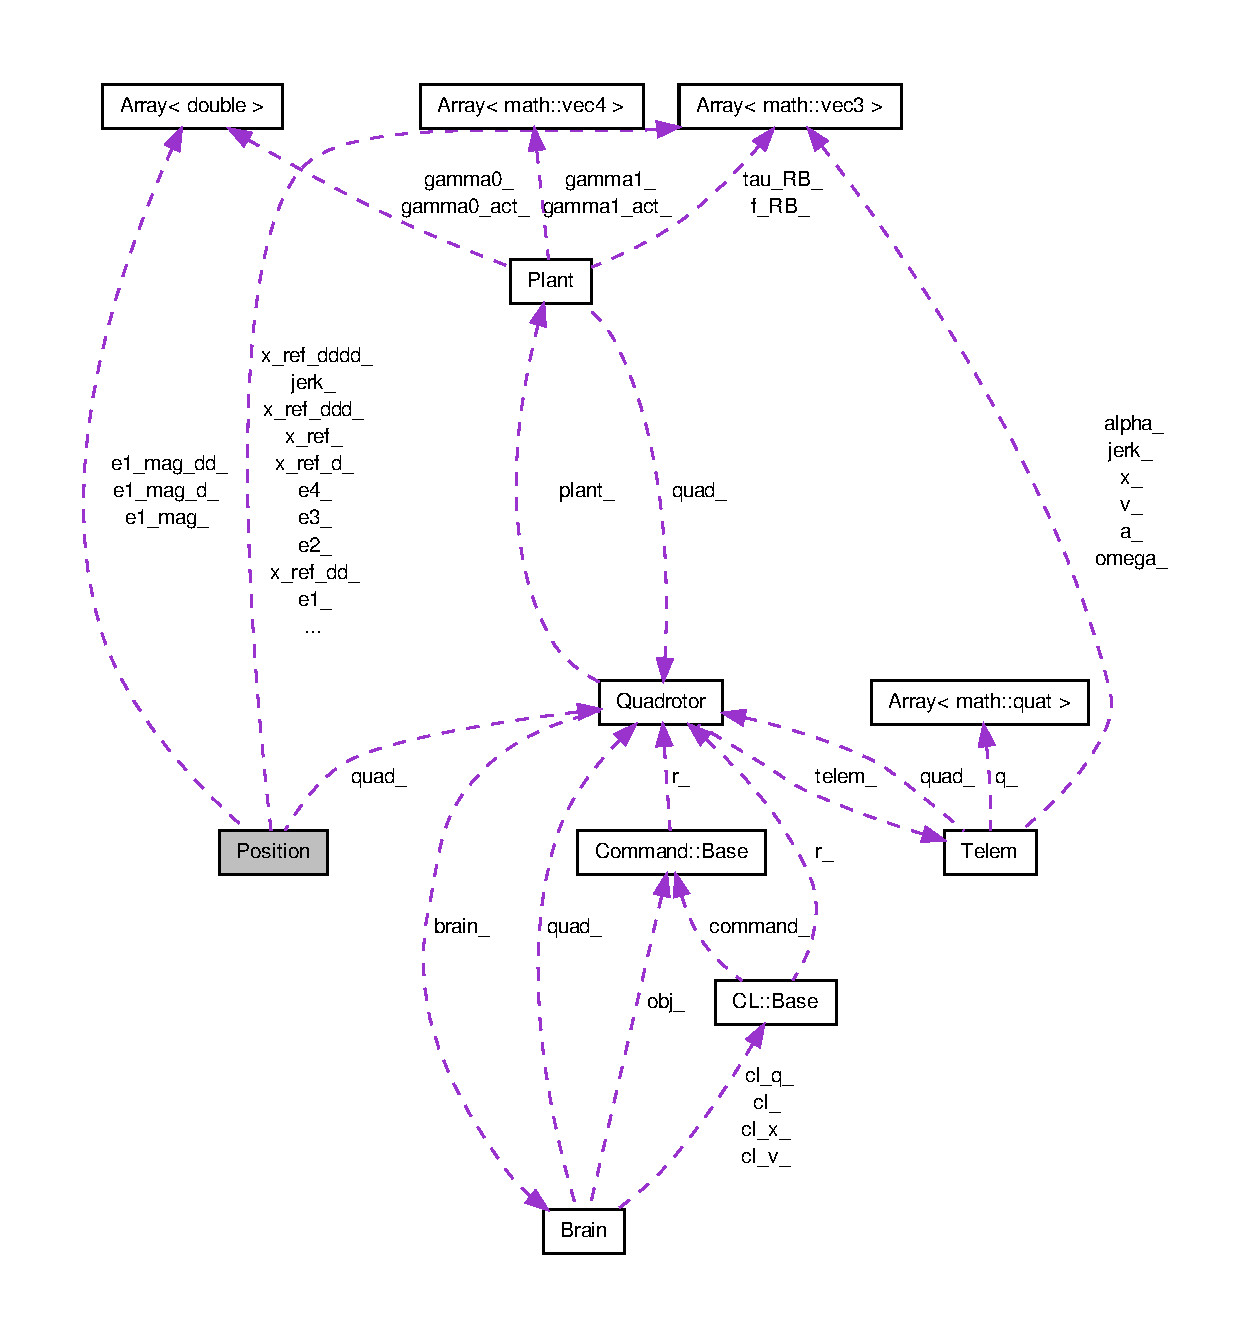
\includegraphics[width=350pt]{classPosition__coll__graph}
\end{center}
\end{figure}
\subsection*{\-Public \-Member \-Functions}
\begin{DoxyCompactItemize}
\item 
\hypertarget{classPosition_a21dc157ba98b5d2611370bf3f349736a}{{\bfseries \-Position} (\hyperlink{classQuadrotor}{\-Quadrotor} $\ast$)}\label{classPosition_a21dc157ba98b5d2611370bf3f349736a}

\item 
\hypertarget{classPosition_a3edff02174569169d30df5b451eebda0}{void {\bfseries reset} ()}\label{classPosition_a3edff02174569169d30df5b451eebda0}

\item 
\hypertarget{classPosition_a924a092bf7875bdbcdc2e82003f4a115}{void {\bfseries fill\-\_\-xref} (int ti1, math\-::vec3 x)}\label{classPosition_a924a092bf7875bdbcdc2e82003f4a115}

\item 
\hypertarget{classPosition_a7dcec18ff9b16b1f239ff4b2186af9da}{void {\bfseries fill\-\_\-xref\-\_\-parametric} (int ti1, math\-::vec3($\ast$f)(double))}\label{classPosition_a7dcec18ff9b16b1f239ff4b2186af9da}

\item 
\hypertarget{classPosition_aba6365e7fe72d0640ad071c804099b34}{void {\bfseries set\-\_\-poles} (double $\ast$)}\label{classPosition_aba6365e7fe72d0640ad071c804099b34}

\item 
\hypertarget{classPosition_a6953d71c48f37e8e761ee97a127e1187}{void {\bfseries step} (double dt, int ti, int ti\-\_\-0)}\label{classPosition_a6953d71c48f37e8e761ee97a127e1187}

\item 
\hypertarget{classPosition_a0f0e34c5613c19185eccd70e61208dfd}{void {\bfseries step\-\_\-accel} (double dt, int ti, int ti\-\_\-0)}\label{classPosition_a0f0e34c5613c19185eccd70e61208dfd}

\item 
\hypertarget{classPosition_a61b9bee4144b6561f6f4bcdf7450033c}{void {\bfseries step\-\_\-jerk} (double dt, int ti, int ti\-\_\-0)}\label{classPosition_a61b9bee4144b6561f6f4bcdf7450033c}

\item 
\hypertarget{classPosition_aba8e066dbbecd1884a25a7805b497b74}{void {\bfseries step\-\_\-jounce} (double dt, int ti, int ti\-\_\-0)}\label{classPosition_aba8e066dbbecd1884a25a7805b497b74}

\item 
\hypertarget{classPosition_a7c4796a6c9d51c12c9a391342bbdb694}{void {\bfseries check\-\_\-command} (int)}\label{classPosition_a7c4796a6c9d51c12c9a391342bbdb694}

\item 
\hypertarget{classPosition_a648d9248f431a97397b46377fe238240}{void {\bfseries write} (int n=0)}\label{classPosition_a648d9248f431a97397b46377fe238240}

\item 
\hypertarget{classPosition_a3b075f928cf1342c1a24e4bb60ca15c4}{void {\bfseries write\-\_\-param} ()}\label{classPosition_a3b075f928cf1342c1a24e4bb60ca15c4}

\item 
\hypertarget{classPosition_a8d9ac8c5c242abc786710f12eec6f384}{void {\bfseries read\-\_\-param} ()}\label{classPosition_a8d9ac8c5c242abc786710f12eec6f384}

\end{DoxyCompactItemize}
\subsection*{\-Public \-Attributes}
\begin{DoxyCompactItemize}
\item 
\hypertarget{classPosition_a0656960cbb357fe00e72e2e3defbaa2d}{\hyperlink{classQuadrotor}{\-Quadrotor} $\ast$ {\bfseries quad\-\_\-}}\label{classPosition_a0656960cbb357fe00e72e2e3defbaa2d}

\item 
\hypertarget{classPosition_ab33c65d8652147d47bc7a39125da09d4}{math\-::mat33 {\bfseries \-C1\-\_\-}}\label{classPosition_ab33c65d8652147d47bc7a39125da09d4}

\item 
\hypertarget{classPosition_a2b15162f8175dfce55897a45a0143e3c}{math\-::mat33 {\bfseries \-C2\-\_\-}}\label{classPosition_a2b15162f8175dfce55897a45a0143e3c}

\item 
\hypertarget{classPosition_a6a3624589f48a6bea858942d4fb28878}{math\-::mat33 {\bfseries \-C3\-\_\-}}\label{classPosition_a6a3624589f48a6bea858942d4fb28878}

\item 
\hypertarget{classPosition_a465a117d632587e74d2890ba4e692219}{math\-::mat33 {\bfseries \-C4\-\_\-}}\label{classPosition_a465a117d632587e74d2890ba4e692219}

\item 
\hypertarget{classPosition_a5f98bd98f4feb7a8702756c23fa9317d}{math\-::mat33 {\bfseries \-C5\-\_\-}}\label{classPosition_a5f98bd98f4feb7a8702756c23fa9317d}

\item 
\hypertarget{classPosition_a3e20810903f953808fe5d3dd4d595dde}{\hyperlink{classArray}{\-Array}$<$ math\-::vec3 $>$ {\bfseries e1\-\_\-}}\label{classPosition_a3e20810903f953808fe5d3dd4d595dde}

\item 
\hypertarget{classPosition_a5da3b18514d8b06e20282d7babf09767}{\hyperlink{classArray}{\-Array}$<$ math\-::vec3 $>$ {\bfseries e2\-\_\-}}\label{classPosition_a5da3b18514d8b06e20282d7babf09767}

\item 
\hypertarget{classPosition_a2cd35aa662a39bacc5644b3dd44f79bf}{\hyperlink{classArray}{\-Array}$<$ math\-::vec3 $>$ {\bfseries e3\-\_\-}}\label{classPosition_a2cd35aa662a39bacc5644b3dd44f79bf}

\item 
\hypertarget{classPosition_ad4a0dcef6b9de3a2941f3bc7cfef9479}{\hyperlink{classArray}{\-Array}$<$ math\-::vec3 $>$ {\bfseries e4\-\_\-}}\label{classPosition_ad4a0dcef6b9de3a2941f3bc7cfef9479}

\item 
\hypertarget{classPosition_a25240c7791a6f2fb7d56fb75a1fe0057}{\hyperlink{classArray}{\-Array}$<$ math\-::vec3 $>$ {\bfseries chi\-\_\-}}\label{classPosition_a25240c7791a6f2fb7d56fb75a1fe0057}

\item 
\hypertarget{classPosition_a453f84b8f10366a3440aa2fe31d23b94}{\hyperlink{classArray}{\-Array}$<$ double $>$ {\bfseries e1\-\_\-mag\-\_\-}}\label{classPosition_a453f84b8f10366a3440aa2fe31d23b94}

\item 
\hypertarget{classPosition_af5aa8548d90fd924f1c5b6e69a7c251c}{\hyperlink{classArray}{\-Array}$<$ double $>$ {\bfseries e1\-\_\-mag\-\_\-d\-\_\-}}\label{classPosition_af5aa8548d90fd924f1c5b6e69a7c251c}

\item 
\hypertarget{classPosition_a2e48aa4120a4c195adc2a62afb457564}{\hyperlink{classArray}{\-Array}$<$ double $>$ {\bfseries e1\-\_\-mag\-\_\-dd\-\_\-}}\label{classPosition_a2e48aa4120a4c195adc2a62afb457564}

\item 
\hypertarget{classPosition_afca069f6a55886ecadb22ca8cfda075a}{\hyperlink{classArray}{\-Array}$<$ math\-::vec3 $>$ {\bfseries x\-\_\-ref\-\_\-}}\label{classPosition_afca069f6a55886ecadb22ca8cfda075a}

\item 
\hypertarget{classPosition_acc04bc1f1e75c1a026f1f8edd1d2e1d7}{\hyperlink{classArray}{\-Array}$<$ math\-::vec3 $>$ {\bfseries x\-\_\-ref\-\_\-d\-\_\-}}\label{classPosition_acc04bc1f1e75c1a026f1f8edd1d2e1d7}

\item 
\hypertarget{classPosition_a11ea8e2d8a54db2c08cfd320ffc702d0}{\hyperlink{classArray}{\-Array}$<$ math\-::vec3 $>$ {\bfseries x\-\_\-ref\-\_\-dd\-\_\-}}\label{classPosition_a11ea8e2d8a54db2c08cfd320ffc702d0}

\item 
\hypertarget{classPosition_a51803cae75d1767f1f38e656ab80b3b8}{\hyperlink{classArray}{\-Array}$<$ math\-::vec3 $>$ {\bfseries x\-\_\-ref\-\_\-ddd\-\_\-}}\label{classPosition_a51803cae75d1767f1f38e656ab80b3b8}

\item 
\hypertarget{classPosition_afb3b7d9b235abd769c0adbff4225fef1}{\hyperlink{classArray}{\-Array}$<$ math\-::vec3 $>$ {\bfseries x\-\_\-ref\-\_\-dddd\-\_\-}}\label{classPosition_afb3b7d9b235abd769c0adbff4225fef1}

\item 
\hypertarget{classPosition_a120045c4cd1e2c9a4f1f7a3587681b1f}{\hyperlink{classArray}{\-Array}$<$ math\-::vec3 $>$ {\bfseries a\-\_\-}}\label{classPosition_a120045c4cd1e2c9a4f1f7a3587681b1f}

\item 
\hypertarget{classPosition_af739ad03cbe3d29eee7aa0631d1e3c1f}{\hyperlink{classArray}{\-Array}$<$ math\-::vec3 $>$ {\bfseries jerk\-\_\-}}\label{classPosition_af739ad03cbe3d29eee7aa0631d1e3c1f}

\item 
\hypertarget{classPosition_a5f22c101e8a63183849a30ede8308b04}{\hyperlink{classArray}{\-Array}$<$ math\-::vec3 $>$ {\bfseries jounce\-\_\-}}\label{classPosition_a5f22c101e8a63183849a30ede8308b04}

\item 
\hypertarget{classPosition_a940b73c924b7a90b293f733ea168da7e}{unsigned int {\bfseries flag\-\_\-}}\label{classPosition_a940b73c924b7a90b293f733ea168da7e}

\end{DoxyCompactItemize}


\-The documentation for this class was generated from the following files\-:\begin{DoxyCompactItemize}
\item 
src/quadrotor/position.\-h\item 
src/quadrotor/position.\-cpp\end{DoxyCompactItemize}

\hypertarget{classCommand_1_1Q}{
\section{Command::Q Class Reference}
\label{classCommand_1_1Q}\index{Command::Q@{Command::Q}}
}
Inheritance diagram for Command::Q:Collaboration diagram for Command::Q:\subsection*{Public Member Functions}
\begin{DoxyCompactItemize}
\item 
\hypertarget{classCommand_1_1Q_a4eb218eafdd864d06a92afc16eb9fee9}{
{\bfseries Q} (\hyperlink{classQuadrotor}{Quadrotor} $\ast$, \hyperlink{classInput_1_1Quat}{Input::Quat} $\ast$)}
\label{classCommand_1_1Q_a4eb218eafdd864d06a92afc16eb9fee9}

\end{DoxyCompactItemize}
\subsection*{Public Attributes}
\begin{DoxyCompactItemize}
\item 
\hypertarget{classCommand_1_1Q_a01f5997c671688955fc024b845ab9689}{
\hyperlink{classInput_1_1Quat}{Input::Quat} $\ast$ {\bfseries in\_\-}}
\label{classCommand_1_1Q_a01f5997c671688955fc024b845ab9689}

\end{DoxyCompactItemize}


The documentation for this class was generated from the following files:\begin{DoxyCompactItemize}
\item 
src/quadrotor/command.h\item 
src/quadrotor/command.cpp\end{DoxyCompactItemize}

\hypertarget{classAlpha1_1_1Q}{
\section{Alpha1::Q Class Reference}
\label{classAlpha1_1_1Q}\index{Alpha1::Q@{Alpha1::Q}}
}
Inheritance diagram for Alpha1::Q:Collaboration diagram for Alpha1::Q:\subsection*{Public Member Functions}
\begin{DoxyCompactItemize}
\item 
\hypertarget{classAlpha1_1_1Q_a5c0a4a0d93f91068ba3157fd23b5e9ee}{
{\bfseries Q} (\hyperlink{classQuadrotor}{Quadrotor} $\ast$r)}
\label{classAlpha1_1_1Q_a5c0a4a0d93f91068ba3157fd23b5e9ee}

\item 
\hypertarget{classAlpha1_1_1Q_ac3f815ffaeb081809f36870cc27c39c1}{
void {\bfseries Step} (int i, double h)}
\label{classAlpha1_1_1Q_ac3f815ffaeb081809f36870cc27c39c1}

\item 
\hypertarget{classAlpha1_1_1Q_a5aeb733bd457272c4aadcb954461b071}{
bool {\bfseries Check} (int, math::vec3)}
\label{classAlpha1_1_1Q_a5aeb733bd457272c4aadcb954461b071}

\item 
\hypertarget{classAlpha1_1_1Q_a2d5895d825723a46858f38bbfb3fa1a0}{
virtual void {\bfseries write} (int)}
\label{classAlpha1_1_1Q_a2d5895d825723a46858f38bbfb3fa1a0}

\item 
\hypertarget{classAlpha1_1_1Q_a41dfc4912bed18a371c98b3046441e59}{
virtual void {\bfseries alloc} (int)}
\label{classAlpha1_1_1Q_a41dfc4912bed18a371c98b3046441e59}

\end{DoxyCompactItemize}


The documentation for this class was generated from the following files:\begin{DoxyCompactItemize}
\item 
src/quadrotor/ControlLaw/Alpha.h\item 
src/quadrotor/ControlLaw/Alpha.cpp\end{DoxyCompactItemize}

\hypertarget{classCL_1_1Q}{
\section{CL::Q$<$ N $>$ Class Template Reference}
\label{classCL_1_1Q}\index{CL::Q@{CL::Q}}
}
Inheritance diagram for CL::Q$<$ N $>$:Collaboration diagram for CL::Q$<$ N $>$:\subsection*{Public Member Functions}
\begin{DoxyCompactItemize}
\item 
\hypertarget{classCL_1_1Q_a557703c167bbb4032c6f5a3776ddd126}{
{\bfseries Q} (\hyperlink{classQuadrotor}{Quadrotor} $\ast$r)}
\label{classCL_1_1Q_a557703c167bbb4032c6f5a3776ddd126}

\item 
\hypertarget{classCL_1_1Q_a42ada1340b7ea8c18d4466b765a81c1f}{
virtual void {\bfseries write} (int n)}
\label{classCL_1_1Q_a42ada1340b7ea8c18d4466b765a81c1f}

\item 
\hypertarget{classCL_1_1Q_aaeb1c2b8db39ba2673f60027cf034cc8}{
virtual void {\bfseries alloc} (int n)}
\label{classCL_1_1Q_aaeb1c2b8db39ba2673f60027cf034cc8}

\end{DoxyCompactItemize}
\subsection*{Public Attributes}
\begin{DoxyCompactItemize}
\item 
\hypertarget{classCL_1_1Q_a1280b14c80c8b20c412a238eedb2ff6c}{
\hyperlink{classArray}{Array}$<$ math::quat $>$ {\bfseries q\_\-ref\_\-}}
\label{classCL_1_1Q_a1280b14c80c8b20c412a238eedb2ff6c}

\item 
\hypertarget{classCL_1_1Q_af7862277ebb36e485ca19c4bb3e8bdcd}{
\hyperlink{classArray}{Array}$<$ math::vec3 $>$ {\bfseries q\_\-ref\_\-\_\-} \mbox{[}N\mbox{]}}
\label{classCL_1_1Q_af7862277ebb36e485ca19c4bb3e8bdcd}

\end{DoxyCompactItemize}
\subsubsection*{template$<$int N$>$ class CL::Q$<$ N $>$}



The documentation for this class was generated from the following file:\begin{DoxyCompactItemize}
\item 
src/quadrotor/ControlLaw/ControlLaw.h\end{DoxyCompactItemize}

\hypertarget{classCommand_1_1Stop_1_1QSettle}{\section{\-Command\-:\-:\-Stop\-:\-:\-Q\-Settle \-Class \-Reference}
\label{classCommand_1_1Stop_1_1QSettle}\index{\-Command\-::\-Stop\-::\-Q\-Settle@{\-Command\-::\-Stop\-::\-Q\-Settle}}
}


\-Inheritance diagram for \-Command\-:\-:\-Stop\-:\-:\-Q\-Settle\-:\nopagebreak
\begin{figure}[H]
\begin{center}
\leavevmode
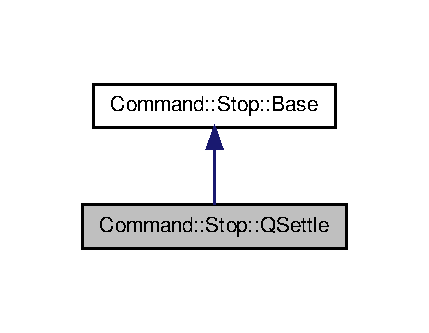
\includegraphics[width=206pt]{classCommand_1_1Stop_1_1QSettle__inherit__graph}
\end{center}
\end{figure}


\-Collaboration diagram for \-Command\-:\-:\-Stop\-:\-:\-Q\-Settle\-:\nopagebreak
\begin{figure}[H]
\begin{center}
\leavevmode
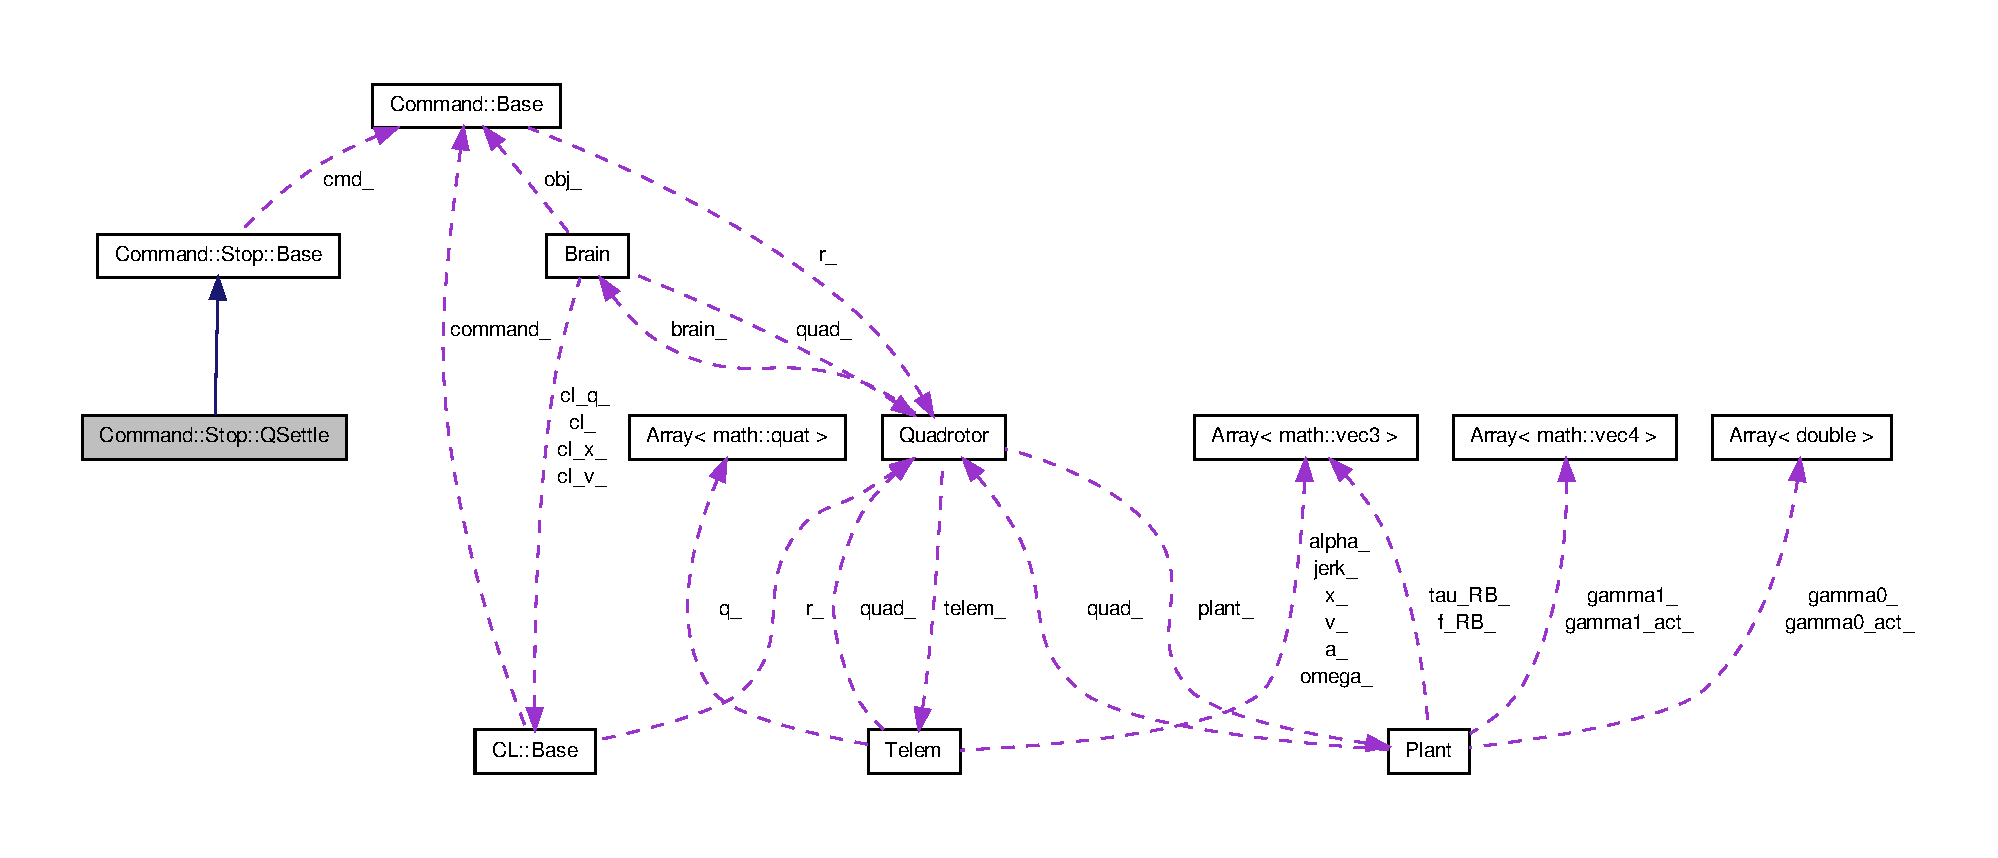
\includegraphics[width=350pt]{classCommand_1_1Stop_1_1QSettle__coll__graph}
\end{center}
\end{figure}
\subsection*{\-Public \-Member \-Functions}
\begin{DoxyCompactItemize}
\item 
\hypertarget{classCommand_1_1Stop_1_1QSettle_a36fc1f9244be5b81c8833243146e1ae9}{{\bfseries \-Q\-Settle} (\hyperlink{classCommand_1_1Base}{\-Command\-::\-Base} $\ast$cmd, double e)}\label{classCommand_1_1Stop_1_1QSettle_a36fc1f9244be5b81c8833243146e1ae9}

\item 
\hypertarget{classCommand_1_1Stop_1_1QSettle_a3c2e37dbd4fdf4cc45fea9014d6cde8e}{virtual void {\bfseries \-Check} (int)}\label{classCommand_1_1Stop_1_1QSettle_a3c2e37dbd4fdf4cc45fea9014d6cde8e}

\end{DoxyCompactItemize}
\subsection*{\-Public \-Attributes}
\begin{DoxyCompactItemize}
\item 
\hypertarget{classCommand_1_1Stop_1_1QSettle_afc557df6532a4071566db3481abd9cb6}{double {\bfseries e\-\_\-}}\label{classCommand_1_1Stop_1_1QSettle_afc557df6532a4071566db3481abd9cb6}

\end{DoxyCompactItemize}


\-The documentation for this class was generated from the following file\-:\begin{DoxyCompactItemize}
\item 
src/quadrotor/command/\-Stop.\-hpp\end{DoxyCompactItemize}

\hypertarget{classQuadrotor}{\section{\-Quadrotor \-Class \-Reference}
\label{classQuadrotor}\index{\-Quadrotor@{\-Quadrotor}}
}


\-Collaboration diagram for \-Quadrotor\-:\nopagebreak
\begin{figure}[H]
\begin{center}
\leavevmode
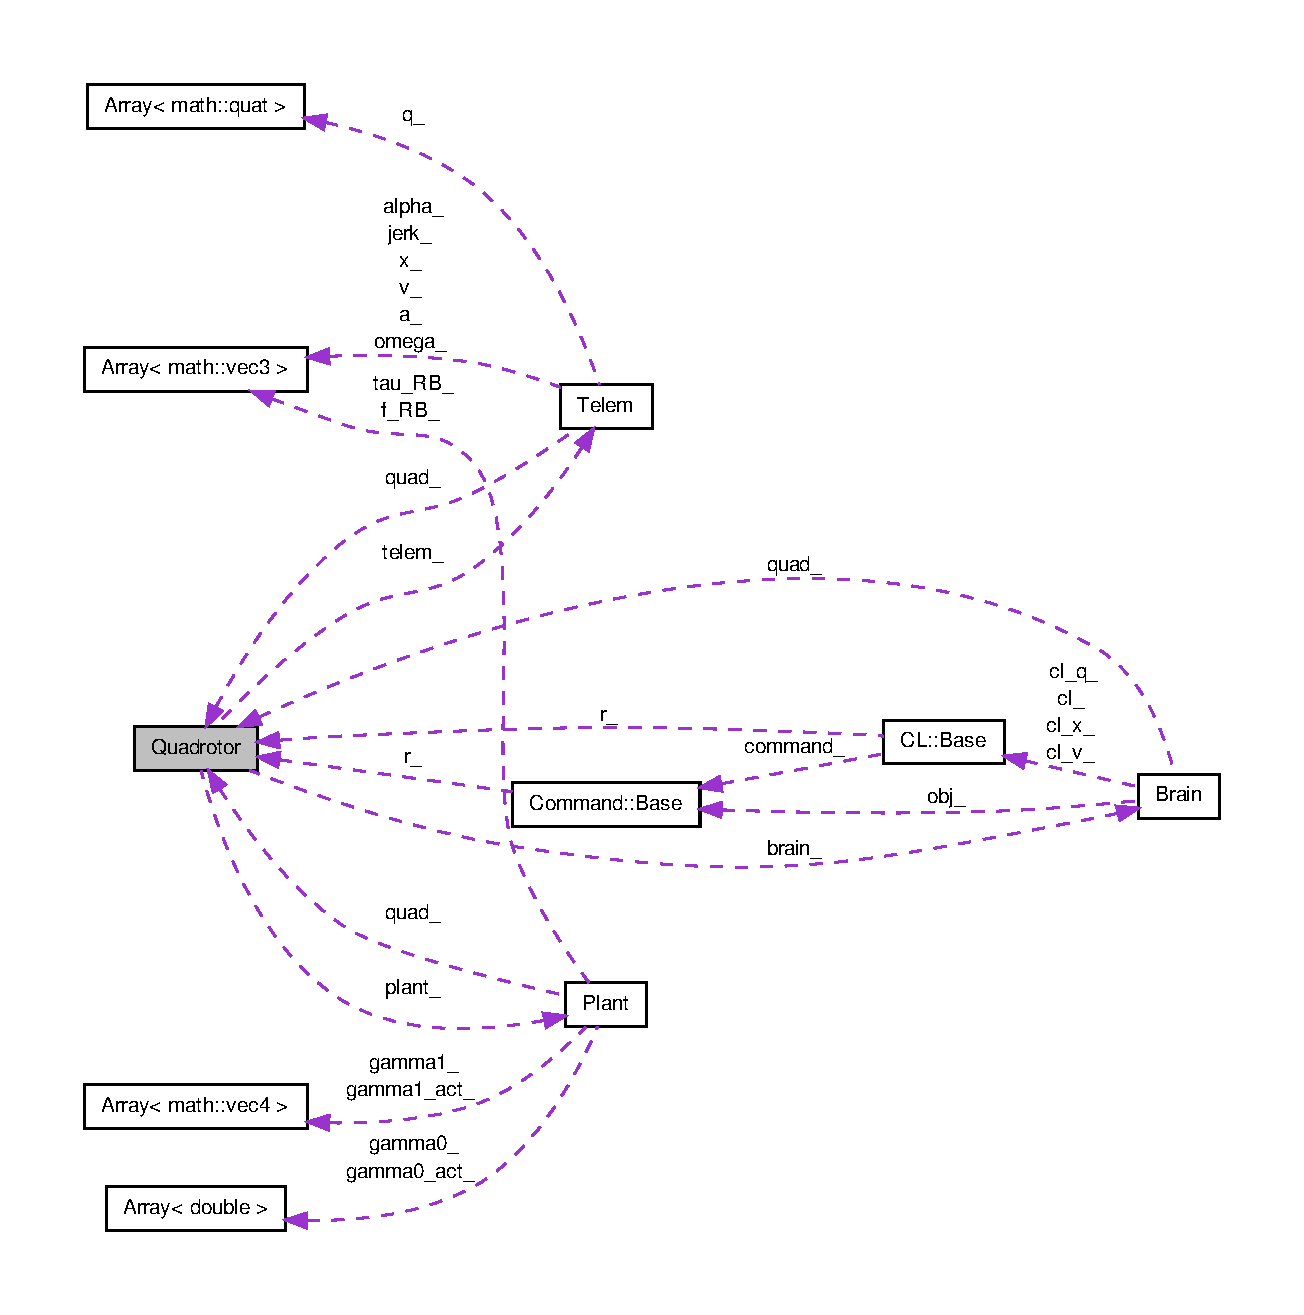
\includegraphics[width=350pt]{classQuadrotor__coll__graph}
\end{center}
\end{figure}
\subsection*{\-Public \-Member \-Functions}
\begin{DoxyCompactItemize}
\item 
\hypertarget{classQuadrotor_a02a4b5c132d374626be48a5d288bb795}{{\bfseries \-Quadrotor} (double dt, int \-N)}\label{classQuadrotor_a02a4b5c132d374626be48a5d288bb795}

\item 
\hypertarget{classQuadrotor_a1e883a0d6205ad9af214afe2b6f84d2f}{void {\bfseries reset} ()}\label{classQuadrotor_a1e883a0d6205ad9af214afe2b6f84d2f}

\item 
\hypertarget{classQuadrotor_a86703e4d10af125e7b34ab09711c80f9}{void {\bfseries run} ()}\label{classQuadrotor_a86703e4d10af125e7b34ab09711c80f9}

\item 
\hypertarget{classQuadrotor_a32c9f06143c6b1ad7eff6442fae29b03}{math\-::vec3 {\bfseries angular\-\_\-accel\-\_\-to\-\_\-torque} (int, math\-::vec3)}\label{classQuadrotor_a32c9f06143c6b1ad7eff6442fae29b03}

\item 
\hypertarget{classQuadrotor_a5ab35934cf51134d5084ee58d9aa63fe}{math\-::vec4 {\bfseries thrust\-\_\-torque\-\_\-to\-\_\-motor\-\_\-speed} (int, double const \&, math\-::vec3 const \&)}\label{classQuadrotor_a5ab35934cf51134d5084ee58d9aa63fe}

\item 
\hypertarget{classQuadrotor_a1c250bf48c42d7fed0f1ebc74dbc7249}{void {\bfseries write} ()}\label{classQuadrotor_a1c250bf48c42d7fed0f1ebc74dbc7249}

\item 
\hypertarget{classQuadrotor_ae35477027bde2e9ad10ef7ac557000a8}{void {\bfseries write\-\_\-param} ()}\label{classQuadrotor_ae35477027bde2e9ad10ef7ac557000a8}

\item 
\hypertarget{classQuadrotor_a65d4670873c532d351a8d06f8c0c79b4}{math\-::vec3 \& {\bfseries x} (int)}\label{classQuadrotor_a65d4670873c532d351a8d06f8c0c79b4}

\item 
\hypertarget{classQuadrotor_aa6c1fd2c44edbb91f813bf0c19e89a80}{math\-::vec3 \& {\bfseries v} (int)}\label{classQuadrotor_aa6c1fd2c44edbb91f813bf0c19e89a80}

\item 
\hypertarget{classQuadrotor_a9b746718f4b7b89a8a764f716a319990}{math\-::vec3 \& {\bfseries a} (int)}\label{classQuadrotor_a9b746718f4b7b89a8a764f716a319990}

\item 
\hypertarget{classQuadrotor_a9434066ee668dbcd0ca298b340ed89c3}{math\-::vec3 \& {\bfseries jerk} (int)}\label{classQuadrotor_a9434066ee668dbcd0ca298b340ed89c3}

\item 
\hypertarget{classQuadrotor_a9983300a030f12958b6fe69e8c001725}{math\-::quat \& {\bfseries q} (int)}\label{classQuadrotor_a9983300a030f12958b6fe69e8c001725}

\item 
\hypertarget{classQuadrotor_a7c087b16e04910c5bdae674a28fedd74}{math\-::vec3 \& {\bfseries omega} (int)}\label{classQuadrotor_a7c087b16e04910c5bdae674a28fedd74}

\item 
\hypertarget{classQuadrotor_ab8b34b70c0636510dd834c617e1cd724}{math\-::vec3 \& {\bfseries alpha} (int)}\label{classQuadrotor_ab8b34b70c0636510dd834c617e1cd724}

\item 
\hypertarget{classQuadrotor_abb1fe86e6ff0db37943602a59e4e0ea9}{double {\bfseries t} (int i) const }\label{classQuadrotor_abb1fe86e6ff0db37943602a59e4e0ea9}

\end{DoxyCompactItemize}
\subsection*{\-Public \-Attributes}
\begin{DoxyCompactItemize}
\item 
\hypertarget{classQuadrotor_ae243377ebb16fc03f32471e45833ca97}{double {\bfseries m\-\_\-}}\label{classQuadrotor_ae243377ebb16fc03f32471e45833ca97}

\item 
\hypertarget{classQuadrotor_abecfcca3af9590e825943cf9cddc692d}{double {\bfseries \-L\-\_\-}}\label{classQuadrotor_abecfcca3af9590e825943cf9cddc692d}

\item 
\hypertarget{classQuadrotor_a77dd677dc966ca2b4cee7ccac6f228fe}{double {\bfseries \-R\-\_\-}}\label{classQuadrotor_a77dd677dc966ca2b4cee7ccac6f228fe}

\item 
\hypertarget{classQuadrotor_a6ec7bcfe228bb7f535603cfbe83dba7b}{double {\bfseries \-Asw\-\_\-}}\label{classQuadrotor_a6ec7bcfe228bb7f535603cfbe83dba7b}

\item 
\hypertarget{classQuadrotor_a83244aa622d512713f6e68b31ed1317c}{double {\bfseries rho\-\_\-}}\label{classQuadrotor_a83244aa622d512713f6e68b31ed1317c}

\item 
\hypertarget{classQuadrotor_a62524b98ee9d7316359c1e947d97212e}{double {\bfseries \-C\-D\-\_\-}}\label{classQuadrotor_a62524b98ee9d7316359c1e947d97212e}

\item 
\hypertarget{classQuadrotor_a2be16b0f0bc98e0ce7fcdce859681c76}{double {\bfseries \-A\-\_\-}}\label{classQuadrotor_a2be16b0f0bc98e0ce7fcdce859681c76}

\item 
\hypertarget{classQuadrotor_a793af63ddb8d77b3dd2d916bbed03707}{double {\bfseries \-Kv\-\_\-}}\label{classQuadrotor_a793af63ddb8d77b3dd2d916bbed03707}

\item 
\hypertarget{classQuadrotor_ab487da82a85c5a703d47daeccd7942a6}{double {\bfseries \-Kt\-\_\-}}\label{classQuadrotor_ab487da82a85c5a703d47daeccd7942a6}

\item 
\hypertarget{classQuadrotor_ae39735df9ee54fdf745136c55c949854}{double {\bfseries \-Ktau\-\_\-}}\label{classQuadrotor_ae39735df9ee54fdf745136c55c949854}

\item 
\hypertarget{classQuadrotor_a95c788dc97935548885b3b5610674584}{double {\bfseries k\-\_\-}}\label{classQuadrotor_a95c788dc97935548885b3b5610674584}

\item 
\hypertarget{classQuadrotor_a1ca9043b119a9d0dd8ffa69124ee7762}{double {\bfseries b\-\_\-}}\label{classQuadrotor_a1ca9043b119a9d0dd8ffa69124ee7762}

\item 
\hypertarget{classQuadrotor_af4f6a0ec758d1775bb9b8233591391ab}{double {\bfseries \-P\-\_\-max\-\_\-}}\label{classQuadrotor_af4f6a0ec758d1775bb9b8233591391ab}

\item 
\hypertarget{classQuadrotor_a7d8e611828d472d90b2a87acd269ec83}{double {\bfseries gamma\-\_\-max\-\_\-}}\label{classQuadrotor_a7d8e611828d472d90b2a87acd269ec83}

\item 
\hypertarget{classQuadrotor_acc5a7c39e99700fa8a46cea815d11ec2}{math\-::mat33 {\bfseries \-I\-\_\-}}\label{classQuadrotor_acc5a7c39e99700fa8a46cea815d11ec2}

\item 
\hypertarget{classQuadrotor_ae242f62c3debf26227bf3be0eb3d3292}{math\-::mat33 {\bfseries \-Iinv\-\_\-}}\label{classQuadrotor_ae242f62c3debf26227bf3be0eb3d3292}

\item 
\hypertarget{classQuadrotor_a95f738e9bce8f5e739c8bb7bd530e21d}{math\-::vec3 {\bfseries gravity\-\_\-}}\label{classQuadrotor_a95f738e9bce8f5e739c8bb7bd530e21d}

\item 
\hypertarget{classQuadrotor_a133a04741751e58cfa64c8c67ef78682}{math\-::mat44 {\bfseries \-A4\-\_\-}}\label{classQuadrotor_a133a04741751e58cfa64c8c67ef78682}

\item 
\hypertarget{classQuadrotor_a822254095092c0c311f0d0f82d45c811}{math\-::mat44 {\bfseries \-A4inv\-\_\-}}\label{classQuadrotor_a822254095092c0c311f0d0f82d45c811}

\item 
\hypertarget{classQuadrotor_a414ecb0b548c0694175d9545856460bc}{double {\bfseries dt\-\_\-}}\label{classQuadrotor_a414ecb0b548c0694175d9545856460bc}

\item 
\hypertarget{classQuadrotor_a55aef1d587c0e0e151a217844869fc97}{int {\bfseries \-N\-\_\-}}\label{classQuadrotor_a55aef1d587c0e0e151a217844869fc97}

\item 
\hypertarget{classQuadrotor_aedbff387d4ec89d5e7464153a24027a6}{double $\ast$ {\bfseries t\-\_\-}}\label{classQuadrotor_aedbff387d4ec89d5e7464153a24027a6}

\item 
\hypertarget{classQuadrotor_a290b8871d95f9adb6005c11540375a17}{int {\bfseries ti\-\_\-stop\-\_\-}}\label{classQuadrotor_a290b8871d95f9adb6005c11540375a17}

\item 
\hypertarget{classQuadrotor_a7eadaf46ba0199a2455274bf4102e68f}{int {\bfseries ti\-\_\-f\-\_\-}}\label{classQuadrotor_a7eadaf46ba0199a2455274bf4102e68f}

\item 
\hypertarget{classQuadrotor_a2ae40aa937f36b17d050d077cf82fa10}{\hyperlink{classTelem}{\-Telem} $\ast$ {\bfseries telem\-\_\-}}\label{classQuadrotor_a2ae40aa937f36b17d050d077cf82fa10}

\item 
\hypertarget{classQuadrotor_a2d994ec0dfa9b08013cce986b1fe10bd}{\hyperlink{classPlant}{\-Plant} $\ast$ {\bfseries plant\-\_\-}}\label{classQuadrotor_a2d994ec0dfa9b08013cce986b1fe10bd}

\item 
\hypertarget{classQuadrotor_ad1dbea34777ea6e3410a94c248ab2455}{\hyperlink{classBrain}{\-Brain} $\ast$ {\bfseries brain\-\_\-}}\label{classQuadrotor_ad1dbea34777ea6e3410a94c248ab2455}

\end{DoxyCompactItemize}


\-The documentation for this class was generated from the following files\-:\begin{DoxyCompactItemize}
\item 
src/quadrotor/quadrotor.\-h\item 
src/quadrotor/quadrotor.\-cpp\end{DoxyCompactItemize}

\hypertarget{classInput_1_1Quat}{\section{\-Input\-:\-:\-Quat \-Class \-Reference}
\label{classInput_1_1Quat}\index{\-Input\-::\-Quat@{\-Input\-::\-Quat}}
}


\-Inheritance diagram for \-Input\-:\-:\-Quat\-:\nopagebreak
\begin{figure}[H]
\begin{center}
\leavevmode
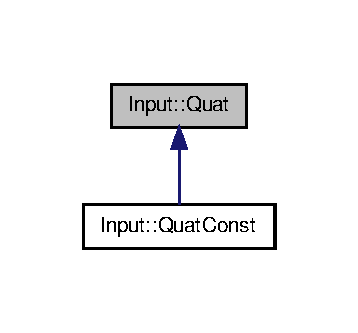
\includegraphics[width=172pt]{classInput_1_1Quat__inherit__graph}
\end{center}
\end{figure}
\subsection*{\-Public \-Member \-Functions}
\begin{DoxyCompactItemize}
\item 
\hypertarget{classInput_1_1Quat_a49bc92df827442db4de31b80928b4b86}{virtual math\-::quat {\bfseries f} (double)=0}\label{classInput_1_1Quat_a49bc92df827442db4de31b80928b4b86}

\end{DoxyCompactItemize}


\-The documentation for this class was generated from the following file\-:\begin{DoxyCompactItemize}
\item 
src/quadrotor/\-Input.\-hpp\end{DoxyCompactItemize}

\hypertarget{classInput_1_1QuatConst}{\section{\-Input\-:\-:\-Quat\-Const \-Class \-Reference}
\label{classInput_1_1QuatConst}\index{\-Input\-::\-Quat\-Const@{\-Input\-::\-Quat\-Const}}
}


\-Inheritance diagram for \-Input\-:\-:\-Quat\-Const\-:\nopagebreak
\begin{figure}[H]
\begin{center}
\leavevmode
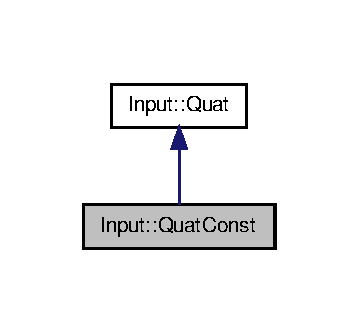
\includegraphics[width=172pt]{classInput_1_1QuatConst__inherit__graph}
\end{center}
\end{figure}


\-Collaboration diagram for \-Input\-:\-:\-Quat\-Const\-:\nopagebreak
\begin{figure}[H]
\begin{center}
\leavevmode
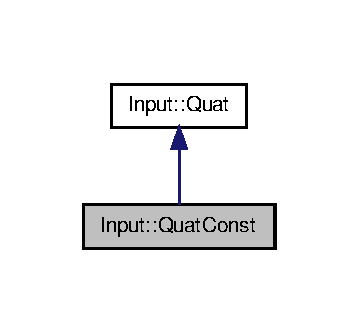
\includegraphics[width=172pt]{classInput_1_1QuatConst__coll__graph}
\end{center}
\end{figure}
\subsection*{\-Public \-Member \-Functions}
\begin{DoxyCompactItemize}
\item 
\hypertarget{classInput_1_1QuatConst_a553b37a3fc9003b0b6eb9d65cb744c66}{{\bfseries \-Quat\-Const} (math\-::quat q)}\label{classInput_1_1QuatConst_a553b37a3fc9003b0b6eb9d65cb744c66}

\item 
\hypertarget{classInput_1_1QuatConst_a94f713bd2ccccdeaa2c2f93ce17db391}{virtual math\-::quat {\bfseries f} (double)}\label{classInput_1_1QuatConst_a94f713bd2ccccdeaa2c2f93ce17db391}

\end{DoxyCompactItemize}
\subsection*{\-Public \-Attributes}
\begin{DoxyCompactItemize}
\item 
\hypertarget{classInput_1_1QuatConst_a256ac5c9c9c3f1ff3967fd3df398e24c}{math\-::quat {\bfseries q\-\_\-}}\label{classInput_1_1QuatConst_a256ac5c9c9c3f1ff3967fd3df398e24c}

\end{DoxyCompactItemize}


\-The documentation for this class was generated from the following file\-:\begin{DoxyCompactItemize}
\item 
src/quadrotor/\-Input.\-hpp\end{DoxyCompactItemize}

\hypertarget{classStopCond}{
\section{StopCond Class Reference}
\label{classStopCond}\index{StopCond@{StopCond}}
}
Inheritance diagram for StopCond:\subsection*{Public Member Functions}
\begin{DoxyCompactItemize}
\item 
\hypertarget{classStopCond_aa359d703fac6691cd13f0b8c4df62d68}{
virtual const char $\ast$ {\bfseries what} () const =0  throw ()}
\label{classStopCond_aa359d703fac6691cd13f0b8c4df62d68}

\end{DoxyCompactItemize}


The documentation for this class was generated from the following file:\begin{DoxyCompactItemize}
\item 
src/quadrotor/except.h\end{DoxyCompactItemize}

\hypertarget{classTelem}{\section{\-Telem \-Class \-Reference}
\label{classTelem}\index{\-Telem@{\-Telem}}
}


\-Collaboration diagram for \-Telem\-:\nopagebreak
\begin{figure}[H]
\begin{center}
\leavevmode
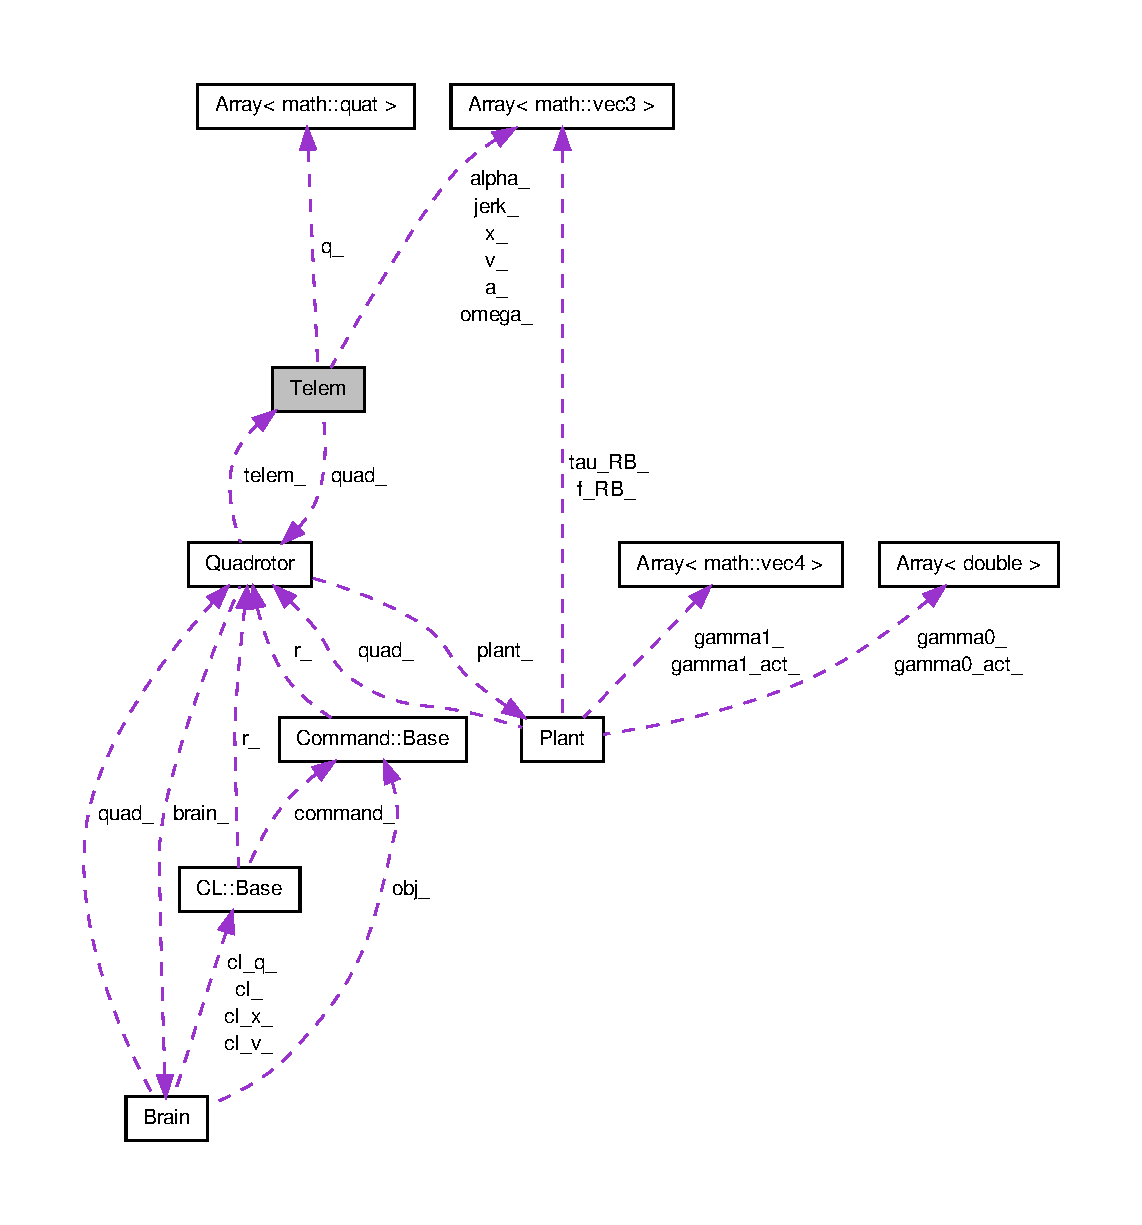
\includegraphics[width=350pt]{classTelem__coll__graph}
\end{center}
\end{figure}
\subsection*{\-Public \-Member \-Functions}
\begin{DoxyCompactItemize}
\item 
\hypertarget{classTelem_adf4c51522fdb2c9e99e4169b0d628f55}{{\bfseries \-Telem} (\hyperlink{classQuadrotor}{\-Quadrotor} $\ast$)}\label{classTelem_adf4c51522fdb2c9e99e4169b0d628f55}

\item 
\hypertarget{classTelem_afaf5327d7f027c91734cbba4a8224569}{void {\bfseries step} (int, double)}\label{classTelem_afaf5327d7f027c91734cbba4a8224569}

\item 
\hypertarget{classTelem_a819ab752690e08d72ea26b8f5eda2995}{void {\bfseries write} (int ti)}\label{classTelem_a819ab752690e08d72ea26b8f5eda2995}

\end{DoxyCompactItemize}
\subsection*{\-Public \-Attributes}
\begin{DoxyCompactItemize}
\item 
\hypertarget{classTelem_a56091fc88e4c6bfe0c9781e2e8be8e44}{\hyperlink{classQuadrotor}{\-Quadrotor} $\ast$ {\bfseries quad\-\_\-}}\label{classTelem_a56091fc88e4c6bfe0c9781e2e8be8e44}

\item 
\hypertarget{classTelem_abdb9ed3d409e996b74909784bf9fd61d}{\hyperlink{classArray}{\-Array}$<$ math\-::quat $>$ {\bfseries q\-\_\-}}\label{classTelem_abdb9ed3d409e996b74909784bf9fd61d}

\item 
\hypertarget{classTelem_a0861519483511babb47b0ffdde4cecf4}{\hyperlink{classArray}{\-Array}$<$ math\-::vec3 $>$ {\bfseries omega\-\_\-}}\label{classTelem_a0861519483511babb47b0ffdde4cecf4}

\item 
\hypertarget{classTelem_a8bb4ed4b578a7a6d90af8e843fe7f907}{\hyperlink{classArray}{\-Array}$<$ math\-::vec3 $>$ {\bfseries alpha\-\_\-}}\label{classTelem_a8bb4ed4b578a7a6d90af8e843fe7f907}

\item 
\hypertarget{classTelem_a59de229401e2fdb33774a18205a3cf71}{\hyperlink{classArray}{\-Array}$<$ math\-::vec3 $>$ {\bfseries x\-\_\-}}\label{classTelem_a59de229401e2fdb33774a18205a3cf71}

\item 
\hypertarget{classTelem_a5767a4b818b4e74f7bccd0bdd7dabf08}{\hyperlink{classArray}{\-Array}$<$ math\-::vec3 $>$ {\bfseries v\-\_\-}}\label{classTelem_a5767a4b818b4e74f7bccd0bdd7dabf08}

\item 
\hypertarget{classTelem_a49f429c0ed1160d4daf2ba6b55b22369}{\hyperlink{classArray}{\-Array}$<$ math\-::vec3 $>$ {\bfseries a\-\_\-}}\label{classTelem_a49f429c0ed1160d4daf2ba6b55b22369}

\item 
\hypertarget{classTelem_ac62fe1671c28ce28b74deb8e94b27c05}{\hyperlink{classArray}{\-Array}$<$ math\-::vec3 $>$ {\bfseries jerk\-\_\-}}\label{classTelem_ac62fe1671c28ce28b74deb8e94b27c05}

\end{DoxyCompactItemize}


\-The documentation for this class was generated from the following files\-:\begin{DoxyCompactItemize}
\item 
src/quadrotor/telem.\-h\item 
src/quadrotor/telem.\-cpp\end{DoxyCompactItemize}

\hypertarget{classCL_1_1Terms}{\section{\-C\-L\-:\-:\-Terms$<$ \-N $>$ \-Class \-Template \-Reference}
\label{classCL_1_1Terms}\index{\-C\-L\-::\-Terms$<$ N $>$@{\-C\-L\-::\-Terms$<$ N $>$}}
}


\-Inheritance diagram for \-C\-L\-:\-:\-Terms$<$ \-N $>$\-:\nopagebreak
\begin{figure}[H]
\begin{center}
\leavevmode
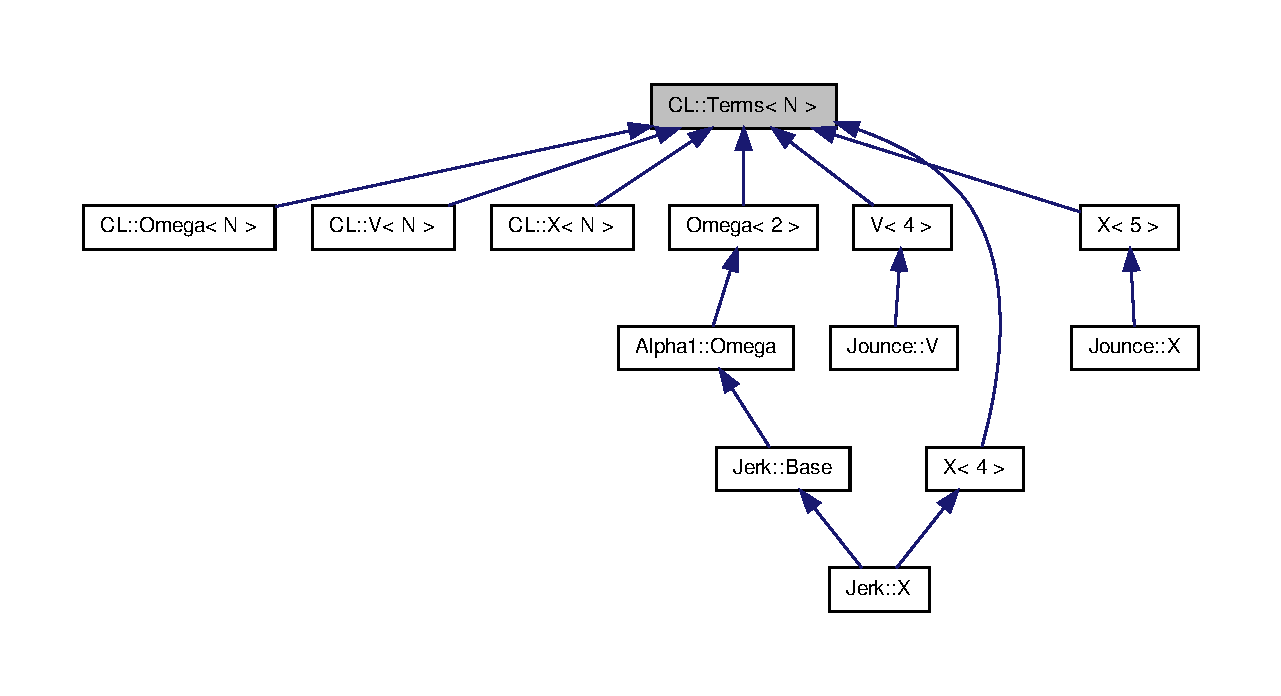
\includegraphics[width=350pt]{classCL_1_1Terms__inherit__graph}
\end{center}
\end{figure}


\-Collaboration diagram for \-C\-L\-:\-:\-Terms$<$ \-N $>$\-:\nopagebreak
\begin{figure}[H]
\begin{center}
\leavevmode
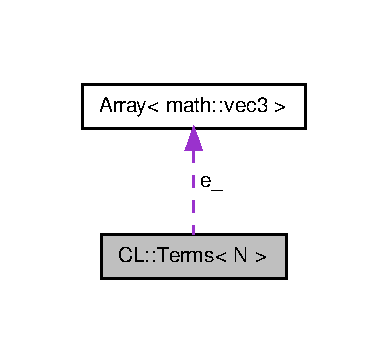
\includegraphics[width=186pt]{classCL_1_1Terms__coll__graph}
\end{center}
\end{figure}
\subsection*{\-Public \-Member \-Functions}
\begin{DoxyCompactItemize}
\item 
\hypertarget{classCL_1_1Terms_a4c473cd263b71294b675216a1ea5cb02}{void {\bfseries set\-\_\-poles} (int $\ast$i, double $\ast$p, int n)}\label{classCL_1_1Terms_a4c473cd263b71294b675216a1ea5cb02}

\item 
\hypertarget{classCL_1_1Terms_a6c45b26f23ec661fb439eb9f0ce567ab}{void {\bfseries set\-\_\-coeff} ()}\label{classCL_1_1Terms_a6c45b26f23ec661fb439eb9f0ce567ab}

\item 
\hypertarget{classCL_1_1Terms_a6aa95892ae24ceadeb80e4d3304bde27}{void {\bfseries write} (int n, \-F\-I\-L\-E $\ast$file)}\label{classCL_1_1Terms_a6aa95892ae24ceadeb80e4d3304bde27}

\item 
\hypertarget{classCL_1_1Terms_af23aca809572dbbf23c02c1abdcc3dce}{void {\bfseries write\-\_\-param} ()}\label{classCL_1_1Terms_af23aca809572dbbf23c02c1abdcc3dce}

\item 
\hypertarget{classCL_1_1Terms_a4aadf66009582c55492bcf52e67813b7}{void {\bfseries read\-\_\-param} ()}\label{classCL_1_1Terms_a4aadf66009582c55492bcf52e67813b7}

\item 
\hypertarget{classCL_1_1Terms_a5bcce9d5baf7d072fc48b1f99008b624}{virtual void {\bfseries alloc} (int n)}\label{classCL_1_1Terms_a5bcce9d5baf7d072fc48b1f99008b624}

\end{DoxyCompactItemize}
\subsection*{\-Public \-Attributes}
\begin{DoxyCompactItemize}
\item 
\hypertarget{classCL_1_1Terms_a140440a957456b8a1444dec9398ebb6e}{math\-::mat33 {\bfseries c\-\_\-} \mbox{[}\-N\mbox{]}}\label{classCL_1_1Terms_a140440a957456b8a1444dec9398ebb6e}

\item 
\hypertarget{classCL_1_1Terms_aea3a6c9598212abff50042ffc62c6616}{\hyperlink{classArray}{\-Array}$<$ math\-::vec3 $>$ {\bfseries e\-\_\-} \mbox{[}\-N\mbox{]}}\label{classCL_1_1Terms_aea3a6c9598212abff50042ffc62c6616}

\item 
\hypertarget{classCL_1_1Terms_aa45b4ef4e3452c250ae7c7132f0cdde7}{double {\bfseries p\-\_\-} \mbox{[}\-N\mbox{]}}\label{classCL_1_1Terms_aa45b4ef4e3452c250ae7c7132f0cdde7}

\end{DoxyCompactItemize}
\subsubsection*{template$<$int \-N$>$ class C\-L\-::\-Terms$<$ N $>$}



\-The documentation for this class was generated from the following file\-:\begin{DoxyCompactItemize}
\item 
src/quadrotor/\-Control\-Law/\-Control\-Law.\-h\end{DoxyCompactItemize}

\hypertarget{classCL_1_1Thrust}{
\section{CL::Thrust Class Reference}
\label{classCL_1_1Thrust}\index{CL::Thrust@{CL::Thrust}}
}
Inheritance diagram for CL::Thrust:Collaboration diagram for CL::Thrust:\subsection*{Public Member Functions}
\begin{DoxyCompactItemize}
\item 
\hypertarget{classCL_1_1Thrust_ab343e53d462e46abc4557aac63e1f2ce}{
{\bfseries Thrust} (\hyperlink{classQuadrotor}{Quadrotor} $\ast$r)}
\label{classCL_1_1Thrust_ab343e53d462e46abc4557aac63e1f2ce}

\item 
\hypertarget{classCL_1_1Thrust_ae30505836a5b53f0611364d9454d8c92}{
virtual void {\bfseries Step} (int, double)}
\label{classCL_1_1Thrust_ae30505836a5b53f0611364d9454d8c92}

\item 
\hypertarget{classCL_1_1Thrust_acf63aa8e59ca8c1e8a0741d4446a0b05}{
virtual void {\bfseries alloc} (int)}
\label{classCL_1_1Thrust_acf63aa8e59ca8c1e8a0741d4446a0b05}

\item 
\hypertarget{classCL_1_1Thrust_a91f80ba432e0e495a6c88613dd34ee2c}{
virtual void {\bfseries write} (int)}
\label{classCL_1_1Thrust_a91f80ba432e0e495a6c88613dd34ee2c}

\end{DoxyCompactItemize}
\subsection*{Public Attributes}
\begin{DoxyCompactItemize}
\item 
\hypertarget{classCL_1_1Thrust_af4783ea1e392716df3866ec1867ee25f}{
\hyperlink{classArray}{Array}$<$ double $>$ {\bfseries thrust\_\-}}
\label{classCL_1_1Thrust_af4783ea1e392716df3866ec1867ee25f}

\end{DoxyCompactItemize}


The documentation for this class was generated from the following files:\begin{DoxyCompactItemize}
\item 
src/quadrotor/ControlLaw/ControlLaw.h\item 
src/quadrotor/ControlLaw/ControlLaw.cpp\end{DoxyCompactItemize}

\hypertarget{classCommand_1_1Stop_1_1Time}{
\section{Command::Stop::Time Class Reference}
\label{classCommand_1_1Stop_1_1Time}\index{Command::Stop::Time@{Command::Stop::Time}}
}
Inheritance diagram for Command::Stop::Time:Collaboration diagram for Command::Stop::Time:\subsection*{Public Member Functions}
\begin{DoxyCompactItemize}
\item 
\hypertarget{classCommand_1_1Stop_1_1Time_a4568ced87aad2d8bb8abcbd0188458d1}{
{\bfseries Time} (\hyperlink{classCommand_1_1Base}{Command::Base} $\ast$cmd, double t)}
\label{classCommand_1_1Stop_1_1Time_a4568ced87aad2d8bb8abcbd0188458d1}

\item 
\hypertarget{classCommand_1_1Stop_1_1Time_ab90dbacde37291aa0f778019bb8c5f6f}{
virtual void {\bfseries Check} (int)}
\label{classCommand_1_1Stop_1_1Time_ab90dbacde37291aa0f778019bb8c5f6f}

\end{DoxyCompactItemize}
\subsection*{Public Attributes}
\begin{DoxyCompactItemize}
\item 
\hypertarget{classCommand_1_1Stop_1_1Time_aad1dfd6b50c86d229b591fd0315b3727}{
double {\bfseries t\_\-}}
\label{classCommand_1_1Stop_1_1Time_aad1dfd6b50c86d229b591fd0315b3727}

\end{DoxyCompactItemize}


The documentation for this class was generated from the following file:\begin{DoxyCompactItemize}
\item 
src/quadrotor/command/Stop.hpp\end{DoxyCompactItemize}

\hypertarget{structCommand_1_1Base_1_1Type}{
\section{Command::Base::Type Struct Reference}
\label{structCommand_1_1Base_1_1Type}\index{Command::Base::Type@{Command::Base::Type}}
}
\subsection*{Public Types}
\begin{DoxyCompactItemize}
\item 
enum {\bfseries e} \{ {\bfseries X}, 
{\bfseries V}, 
{\bfseries Q}, 
{\bfseries FREEZE}
 \}
\end{DoxyCompactItemize}


The documentation for this struct was generated from the following file:\begin{DoxyCompactItemize}
\item 
src/quadrotor/command.h\end{DoxyCompactItemize}

\hypertarget{classCL_1_1V}{\section{\-C\-L\-:\-:\-V$<$ \-N $>$ \-Class \-Template \-Reference}
\label{classCL_1_1V}\index{\-C\-L\-::\-V$<$ N $>$@{\-C\-L\-::\-V$<$ N $>$}}
}


\-Inheritance diagram for \-C\-L\-:\-:\-V$<$ \-N $>$\-:\nopagebreak
\begin{figure}[H]
\begin{center}
\leavevmode
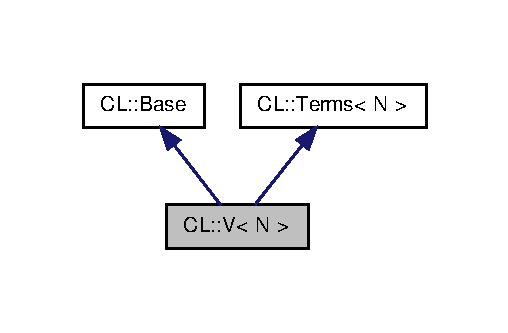
\includegraphics[width=244pt]{classCL_1_1V__inherit__graph}
\end{center}
\end{figure}


\-Collaboration diagram for \-C\-L\-:\-:\-V$<$ \-N $>$\-:\nopagebreak
\begin{figure}[H]
\begin{center}
\leavevmode
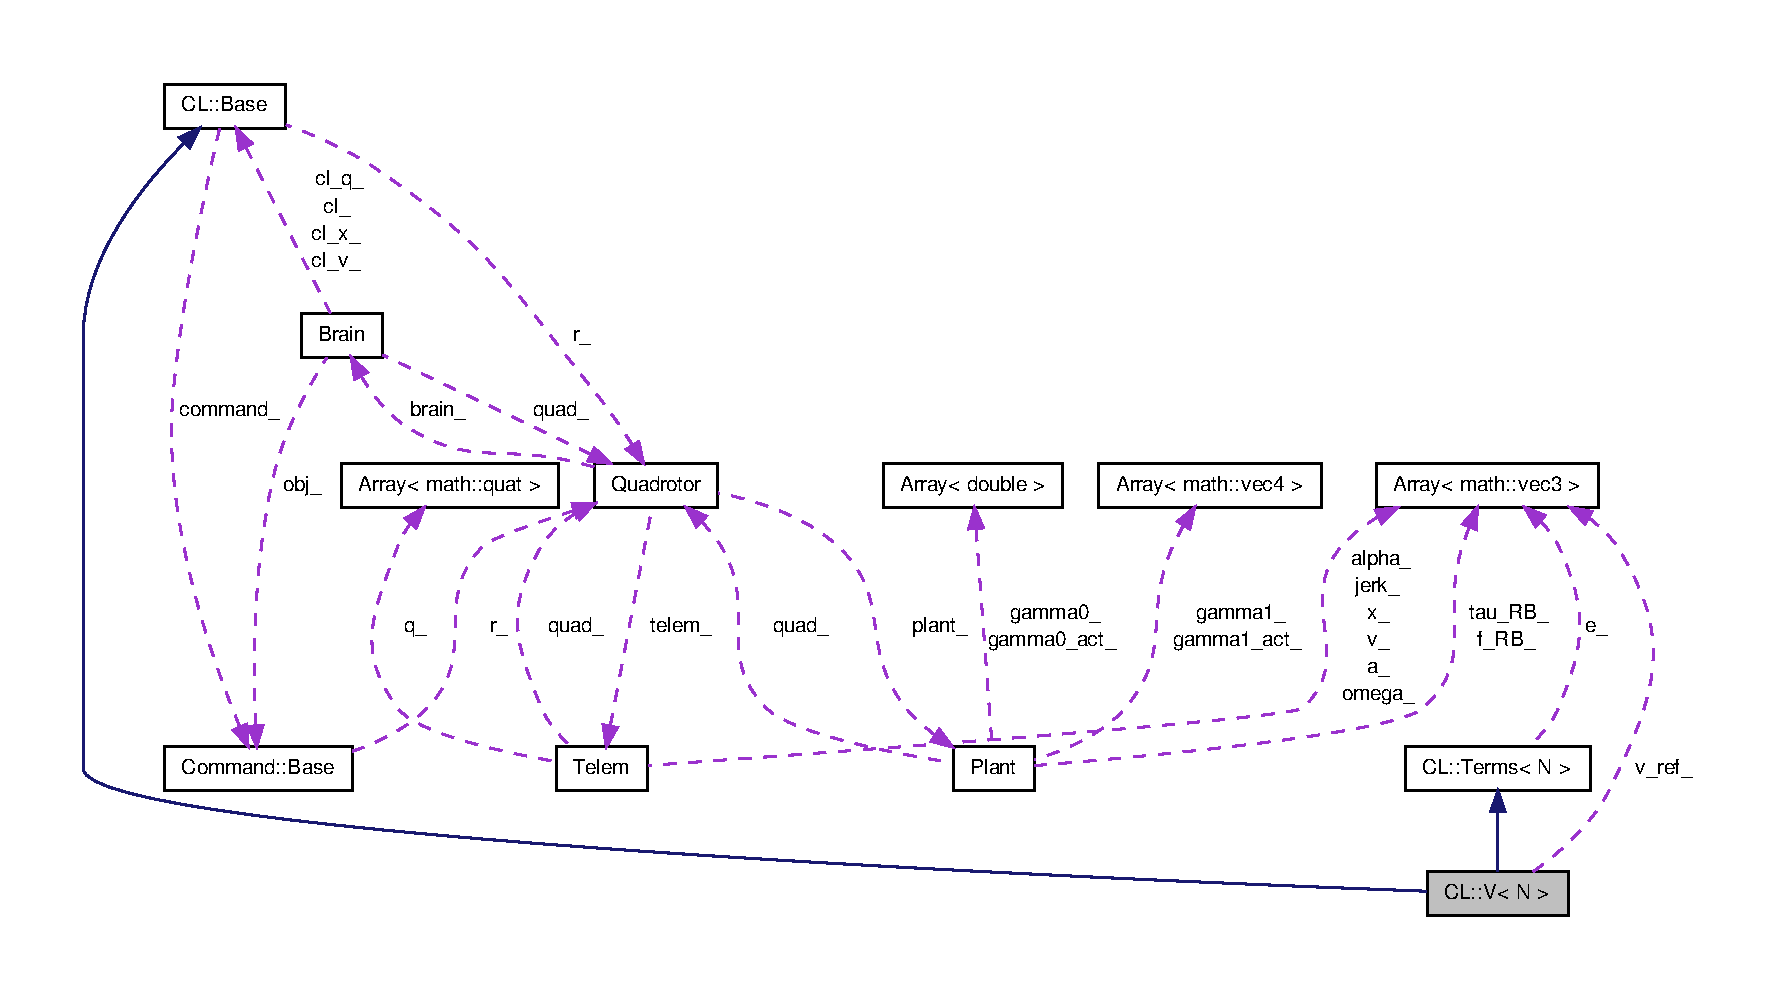
\includegraphics[width=350pt]{classCL_1_1V__coll__graph}
\end{center}
\end{figure}
\subsection*{\-Public \-Member \-Functions}
\begin{DoxyCompactItemize}
\item 
\hypertarget{classCL_1_1V_abebb60fede42f7c660791e66c3bcd7cd}{{\bfseries \-V} (\hyperlink{classQuadrotor}{\-Quadrotor} $\ast$r)}\label{classCL_1_1V_abebb60fede42f7c660791e66c3bcd7cd}

\item 
\hypertarget{classCL_1_1V_ae26d7f9cdd0c82cde2fb483e3adae0e4}{virtual bool {\bfseries \-Check} (int, math\-::vec3)=0}\label{classCL_1_1V_ae26d7f9cdd0c82cde2fb483e3adae0e4}

\item 
\hypertarget{classCL_1_1V_afb721f361ca6c16e2214922fddfd0aa5}{virtual void {\bfseries alloc} (int n)}\label{classCL_1_1V_afb721f361ca6c16e2214922fddfd0aa5}

\item 
\hypertarget{classCL_1_1V_aeec78b8c6a02cc18e4121b6599251275}{virtual void {\bfseries write} (int n)}\label{classCL_1_1V_aeec78b8c6a02cc18e4121b6599251275}

\end{DoxyCompactItemize}
\subsection*{\-Public \-Attributes}
\begin{DoxyCompactItemize}
\item 
\hypertarget{classCL_1_1V_aa556065fca27e51e6a911514a74e0e07}{\hyperlink{classArray}{\-Array}$<$ math\-::vec3 $>$ {\bfseries v\-\_\-ref\-\_\-} \mbox{[}\-N\mbox{]}}\label{classCL_1_1V_aa556065fca27e51e6a911514a74e0e07}

\end{DoxyCompactItemize}
\subsubsection*{template$<$int \-N$>$ class C\-L\-::\-V$<$ N $>$}



\-The documentation for this class was generated from the following file\-:\begin{DoxyCompactItemize}
\item 
src/quadrotor/\-Control\-Law/\-Control\-Law.\-h\end{DoxyCompactItemize}

\hypertarget{classCommand_1_1V}{\section{\-Command\-:\-:\-V \-Class \-Reference}
\label{classCommand_1_1V}\index{\-Command\-::\-V@{\-Command\-::\-V}}
}


\-Inheritance diagram for \-Command\-:\-:\-V\-:\nopagebreak
\begin{figure}[H]
\begin{center}
\leavevmode
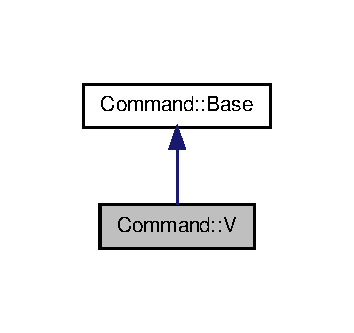
\includegraphics[width=170pt]{classCommand_1_1V__inherit__graph}
\end{center}
\end{figure}


\-Collaboration diagram for \-Command\-:\-:\-V\-:\nopagebreak
\begin{figure}[H]
\begin{center}
\leavevmode
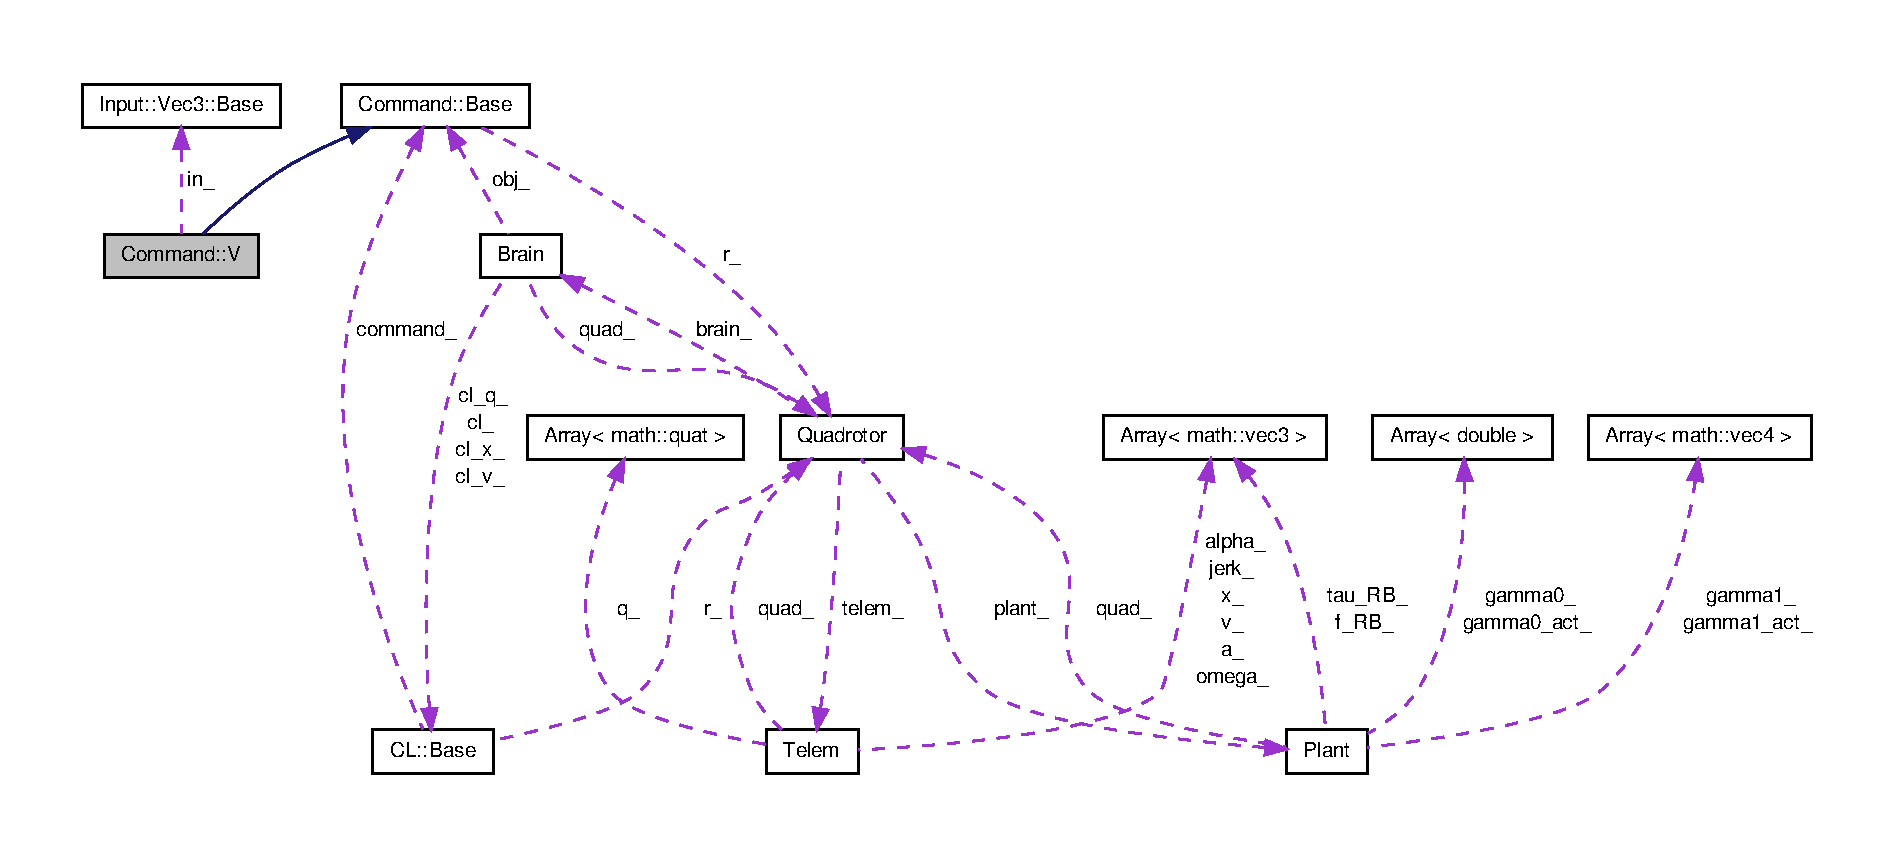
\includegraphics[width=350pt]{classCommand_1_1V__coll__graph}
\end{center}
\end{figure}
\subsection*{\-Public \-Member \-Functions}
\begin{DoxyCompactItemize}
\item 
\hypertarget{classCommand_1_1V_ab0f8e91d15ed03f3b5320314575c65ff}{{\bfseries \-V} (\hyperlink{classQuadrotor}{\-Quadrotor} $\ast$, \hyperlink{classInput_1_1Vec3_1_1Base}{\-Input\-::\-Vec3\-::\-Base} $\ast$)}\label{classCommand_1_1V_ab0f8e91d15ed03f3b5320314575c65ff}

\end{DoxyCompactItemize}
\subsection*{\-Public \-Attributes}
\begin{DoxyCompactItemize}
\item 
\hypertarget{classCommand_1_1V_a5503b80ffdb2daa746bd1d1c6b6c8ffe}{\hyperlink{classInput_1_1Vec3_1_1Base}{\-Input\-::\-Vec3\-::\-Base} $\ast$ {\bfseries in\-\_\-}}\label{classCommand_1_1V_a5503b80ffdb2daa746bd1d1c6b6c8ffe}

\end{DoxyCompactItemize}


\-The documentation for this class was generated from the following files\-:\begin{DoxyCompactItemize}
\item 
src/quadrotor/command.\-h\item 
src/quadrotor/command.\-cpp\end{DoxyCompactItemize}

\hypertarget{classJounce_1_1V}{
\section{Jounce::V Class Reference}
\label{classJounce_1_1V}\index{Jounce::V@{Jounce::V}}
}
Inheritance diagram for Jounce::V:Collaboration diagram for Jounce::V:\subsection*{Public Member Functions}
\begin{DoxyCompactItemize}
\item 
\hypertarget{classJounce_1_1V_a1cb67cc154796091ff5b571b0cafa184}{
{\bfseries V} (\hyperlink{classQuadrotor}{Quadrotor} $\ast$r)}
\label{classJounce_1_1V_a1cb67cc154796091ff5b571b0cafa184}

\item 
\hypertarget{classJounce_1_1V_a51b032ee7b0f6bf93f28c764ea117c11}{
virtual void {\bfseries Step} (int, double)}
\label{classJounce_1_1V_a51b032ee7b0f6bf93f28c764ea117c11}

\item 
\hypertarget{classJounce_1_1V_a504f05fe2b80328d863eacddfb15b555}{
virtual bool {\bfseries Check} (int, math::vec3)}
\label{classJounce_1_1V_a504f05fe2b80328d863eacddfb15b555}

\item 
\hypertarget{classJounce_1_1V_af93b8cc4b4609e4b4ee04a635656a0da}{
virtual void {\bfseries alloc} (int)}
\label{classJounce_1_1V_af93b8cc4b4609e4b4ee04a635656a0da}

\item 
\hypertarget{classJounce_1_1V_a25a4b61e80beb56af2a9ad1fc5a1d270}{
virtual void {\bfseries write} (int)}
\label{classJounce_1_1V_a25a4b61e80beb56af2a9ad1fc5a1d270}

\end{DoxyCompactItemize}


The documentation for this class was generated from the following files:\begin{DoxyCompactItemize}
\item 
src/quadrotor/ControlLaw/Jounce.h\item 
src/quadrotor/ControlLaw/Jounce.cpp\end{DoxyCompactItemize}

\hypertarget{classCommand_1_1Stop_1_1VCross}{
\section{Command::Stop::VCross Class Reference}
\label{classCommand_1_1Stop_1_1VCross}\index{Command::Stop::VCross@{Command::Stop::VCross}}
}
Inheritance diagram for Command::Stop::VCross:Collaboration diagram for Command::Stop::VCross:\subsection*{Public Member Functions}
\begin{DoxyCompactItemize}
\item 
\hypertarget{classCommand_1_1Stop_1_1VCross_af8efe94d12d562f53dd32819947b7e16}{
{\bfseries VCross} (\hyperlink{classCommand_1_1Base}{Command::Base} $\ast$cmd, math::plane p)}
\label{classCommand_1_1Stop_1_1VCross_af8efe94d12d562f53dd32819947b7e16}

\item 
\hypertarget{classCommand_1_1Stop_1_1VCross_a973ed85dc311fa2df5d83a78ca8f2b54}{
virtual void {\bfseries Check} (int)}
\label{classCommand_1_1Stop_1_1VCross_a973ed85dc311fa2df5d83a78ca8f2b54}

\end{DoxyCompactItemize}
\subsection*{Public Attributes}
\begin{DoxyCompactItemize}
\item 
\hypertarget{classCommand_1_1Stop_1_1VCross_a910e3731fbe92e4e2faaed5d3488ac9f}{
math::plane {\bfseries p\_\-}}
\label{classCommand_1_1Stop_1_1VCross_a910e3731fbe92e4e2faaed5d3488ac9f}

\item 
\hypertarget{classCommand_1_1Stop_1_1VCross_aa1d7a2990ffcb30d6f4204c4a76959a1}{
double {\bfseries d\_\-}}
\label{classCommand_1_1Stop_1_1VCross_aa1d7a2990ffcb30d6f4204c4a76959a1}

\end{DoxyCompactItemize}


The documentation for this class was generated from the following files:\begin{DoxyCompactItemize}
\item 
src/quadrotor/command/Stop.hpp\item 
src/quadrotor/command/Stop.cpp\end{DoxyCompactItemize}

\hypertarget{classCommand_1_1Stop_1_1VSettle}{
\section{Command::Stop::VSettle Class Reference}
\label{classCommand_1_1Stop_1_1VSettle}\index{Command::Stop::VSettle@{Command::Stop::VSettle}}
}
Inheritance diagram for Command::Stop::VSettle:Collaboration diagram for Command::Stop::VSettle:\subsection*{Public Member Functions}
\begin{DoxyCompactItemize}
\item 
\hypertarget{classCommand_1_1Stop_1_1VSettle_a07fd40d6e22d9368ccd2a471f5ba3f07}{
{\bfseries VSettle} (\hyperlink{classCommand_1_1Base}{Command::Base} $\ast$cmd, math::vec3 e)}
\label{classCommand_1_1Stop_1_1VSettle_a07fd40d6e22d9368ccd2a471f5ba3f07}

\item 
\hypertarget{classCommand_1_1Stop_1_1VSettle_aa8632c09f01cb9427d33571001522fa8}{
virtual void {\bfseries Check} (int)}
\label{classCommand_1_1Stop_1_1VSettle_aa8632c09f01cb9427d33571001522fa8}

\end{DoxyCompactItemize}
\subsection*{Public Attributes}
\begin{DoxyCompactItemize}
\item 
\hypertarget{classCommand_1_1Stop_1_1VSettle_a34a092cedcae2ea8bda7ccc75028345a}{
math::vec3 {\bfseries e\_\-}}
\label{classCommand_1_1Stop_1_1VSettle_a34a092cedcae2ea8bda7ccc75028345a}

\end{DoxyCompactItemize}


The documentation for this class was generated from the following files:\begin{DoxyCompactItemize}
\item 
src/quadrotor/command/Stop.hpp\item 
src/quadrotor/command/Stop.cpp\end{DoxyCompactItemize}

\hypertarget{classJerk_1_1X}{
\section{Jerk::X Class Reference}
\label{classJerk_1_1X}\index{Jerk::X@{Jerk::X}}
}
Inheritance diagram for Jerk::X:Collaboration diagram for Jerk::X:\subsection*{Public Member Functions}
\begin{DoxyCompactItemize}
\item 
\hypertarget{classJerk_1_1X_a49b3ee051b79b0266fbb0666fc79fcd8}{
{\bfseries X} (\hyperlink{classQuadrotor}{Quadrotor} $\ast$)}
\label{classJerk_1_1X_a49b3ee051b79b0266fbb0666fc79fcd8}

\item 
\hypertarget{classJerk_1_1X_a89d9df4dbc31111d148f781d485fa298}{
void {\bfseries step} (int, double)}
\label{classJerk_1_1X_a89d9df4dbc31111d148f781d485fa298}

\item 
\hypertarget{classJerk_1_1X_a9dd460bb611e2a8dbc989491db8f791c}{
virtual bool {\bfseries Check} (int, math::vec3)}
\label{classJerk_1_1X_a9dd460bb611e2a8dbc989491db8f791c}

\item 
\hypertarget{classJerk_1_1X_a4535a7664d3b8180395b8886b7514c92}{
virtual void {\bfseries alloc} (int)=0}
\label{classJerk_1_1X_a4535a7664d3b8180395b8886b7514c92}

\item 
\hypertarget{classJerk_1_1X_af5bf90eacad593adefea4b552e88b8b0}{
virtual void {\bfseries write} (int)}
\label{classJerk_1_1X_af5bf90eacad593adefea4b552e88b8b0}

\end{DoxyCompactItemize}


The documentation for this class was generated from the following files:\begin{DoxyCompactItemize}
\item 
src/quadrotor/ControlLaw/Jerk.h\item 
src/quadrotor/ControlLaw/Jerk.cpp\end{DoxyCompactItemize}

\hypertarget{classJounce_1_1X}{
\section{Jounce::X Class Reference}
\label{classJounce_1_1X}\index{Jounce::X@{Jounce::X}}
}
Inheritance diagram for Jounce::X:Collaboration diagram for Jounce::X:\subsection*{Public Member Functions}
\begin{DoxyCompactItemize}
\item 
\hypertarget{classJounce_1_1X_a8a32e0c522fceca1c238f090f199703f}{
{\bfseries X} (\hyperlink{classQuadrotor}{Quadrotor} $\ast$)}
\label{classJounce_1_1X_a8a32e0c522fceca1c238f090f199703f}

\item 
\hypertarget{classJounce_1_1X_a5517653cfa6e81ceca032d1692e36842}{
bool {\bfseries Check} (int, math::vec3)}
\label{classJounce_1_1X_a5517653cfa6e81ceca032d1692e36842}

\item 
\hypertarget{classJounce_1_1X_aa37ceb36cb1a026f825e02c329f3c56e}{
virtual void {\bfseries Step} (int, double)}
\label{classJounce_1_1X_aa37ceb36cb1a026f825e02c329f3c56e}

\item 
\hypertarget{classJounce_1_1X_a531bc708807c552fbc3d28a6ac0c11a5}{
virtual void {\bfseries alloc} (int)}
\label{classJounce_1_1X_a531bc708807c552fbc3d28a6ac0c11a5}

\item 
\hypertarget{classJounce_1_1X_ad860d72f6b64207c6e8ba9927e1ea55c}{
virtual void {\bfseries write} (int)}
\label{classJounce_1_1X_ad860d72f6b64207c6e8ba9927e1ea55c}

\end{DoxyCompactItemize}


The documentation for this class was generated from the following files:\begin{DoxyCompactItemize}
\item 
src/quadrotor/ControlLaw/Jounce.h\item 
src/quadrotor/ControlLaw/Jounce.cpp\end{DoxyCompactItemize}

\hypertarget{classCL_1_1X}{
\section{CL::X$<$ N $>$ Class Template Reference}
\label{classCL_1_1X}\index{CL::X@{CL::X}}
}
Inheritance diagram for CL::X$<$ N $>$:Collaboration diagram for CL::X$<$ N $>$:\subsection*{Public Member Functions}
\begin{DoxyCompactItemize}
\item 
\hypertarget{classCL_1_1X_ac0df118e23cb6f9fd151c295f20b5dc7}{
{\bfseries X} (\hyperlink{classQuadrotor}{Quadrotor} $\ast$r)}
\label{classCL_1_1X_ac0df118e23cb6f9fd151c295f20b5dc7}

\item 
\hypertarget{classCL_1_1X_aa1a6d63850e96205aead2cf514646b82}{
virtual bool {\bfseries Check} (int, math::vec3)=0}
\label{classCL_1_1X_aa1a6d63850e96205aead2cf514646b82}

\item 
\hypertarget{classCL_1_1X_a54020da1e162b1813e86d4bf919c4da3}{
virtual void {\bfseries alloc} (int n)}
\label{classCL_1_1X_a54020da1e162b1813e86d4bf919c4da3}

\item 
\hypertarget{classCL_1_1X_a7f4029b18e5f19adb12c27aac2210977}{
virtual void {\bfseries write} (int n)}
\label{classCL_1_1X_a7f4029b18e5f19adb12c27aac2210977}

\item 
\hypertarget{classCL_1_1X_a31783ad77e8fe3aca841633c84c396b4}{
virtual void {\bfseries Init} (int i)}
\label{classCL_1_1X_a31783ad77e8fe3aca841633c84c396b4}

\end{DoxyCompactItemize}
\subsection*{Public Attributes}
\begin{DoxyCompactItemize}
\item 
\hypertarget{classCL_1_1X_ae8cca322585bd7d858fb1408ad6d1f72}{
\hyperlink{classArray}{Array}$<$ math::vec3 $>$ {\bfseries x\_\-ref\_\-} \mbox{[}N\mbox{]}}
\label{classCL_1_1X_ae8cca322585bd7d858fb1408ad6d1f72}

\end{DoxyCompactItemize}
\subsubsection*{template$<$int N$>$ class CL::X$<$ N $>$}



The documentation for this class was generated from the following file:\begin{DoxyCompactItemize}
\item 
src/quadrotor/ControlLaw/ControlLaw.h\end{DoxyCompactItemize}

\hypertarget{classCommand_1_1X}{\section{\-Command\-:\-:\-X \-Class \-Reference}
\label{classCommand_1_1X}\index{\-Command\-::\-X@{\-Command\-::\-X}}
}


\-Inheritance diagram for \-Command\-:\-:\-X\-:\nopagebreak
\begin{figure}[H]
\begin{center}
\leavevmode
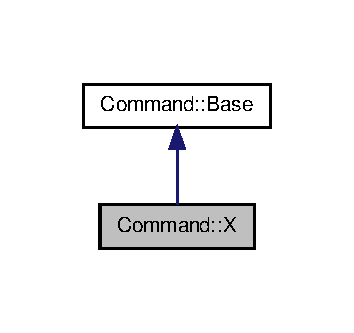
\includegraphics[width=170pt]{classCommand_1_1X__inherit__graph}
\end{center}
\end{figure}


\-Collaboration diagram for \-Command\-:\-:\-X\-:\nopagebreak
\begin{figure}[H]
\begin{center}
\leavevmode
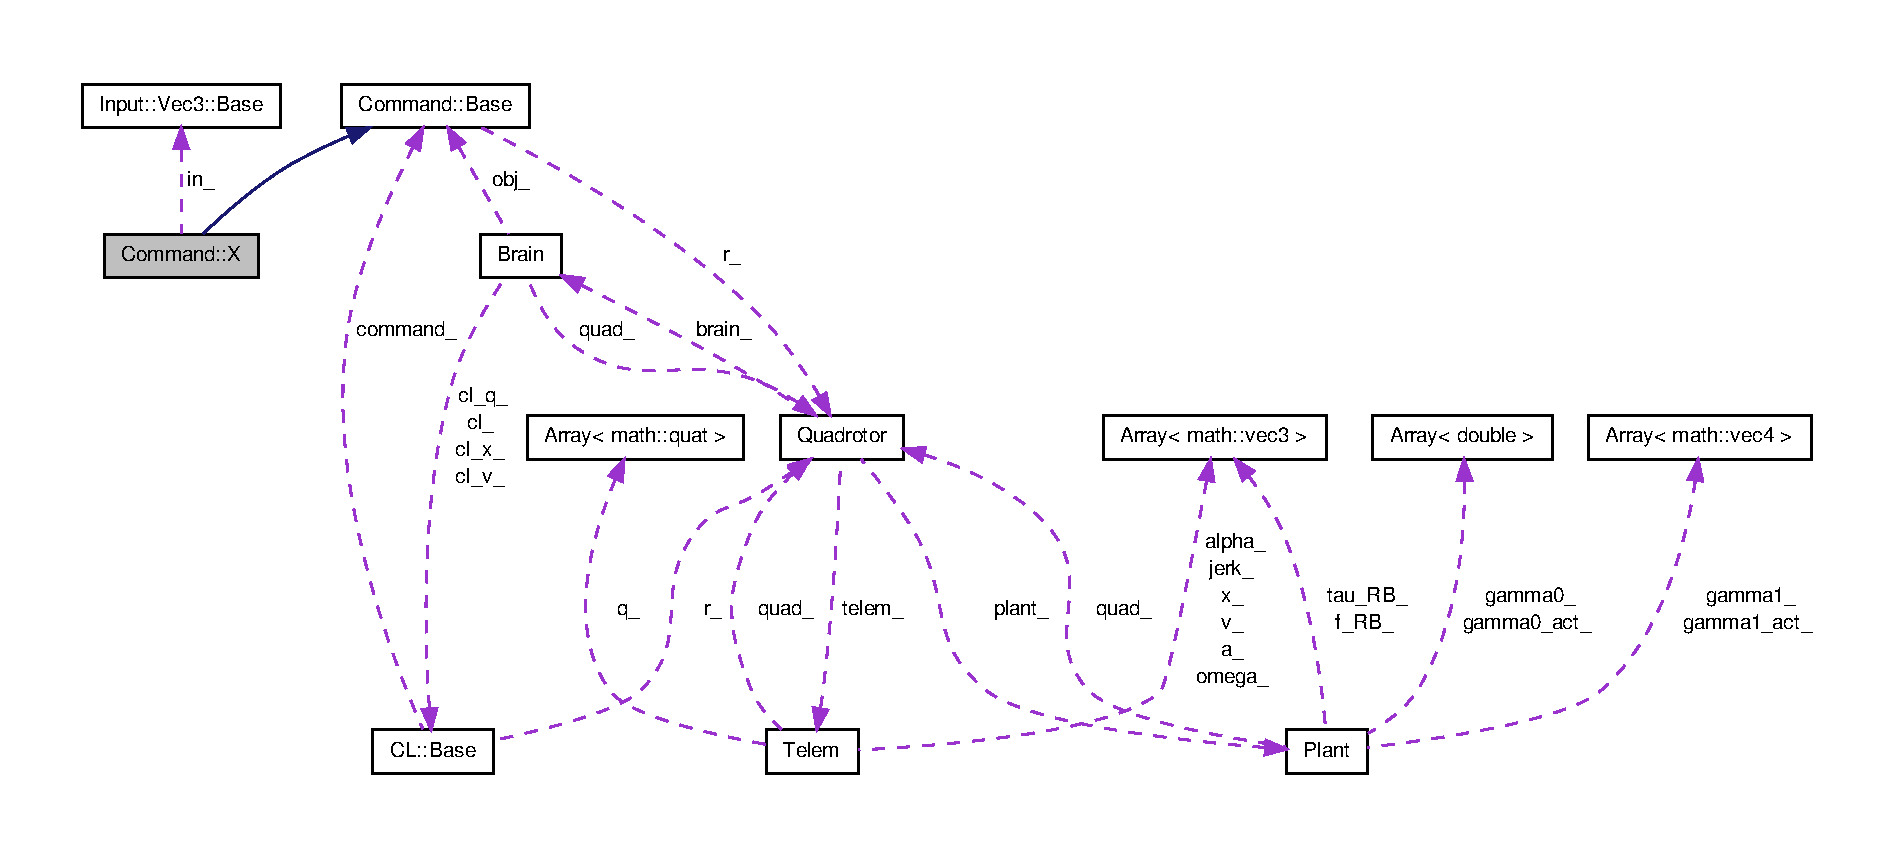
\includegraphics[width=350pt]{classCommand_1_1X__coll__graph}
\end{center}
\end{figure}
\subsection*{\-Public \-Member \-Functions}
\begin{DoxyCompactItemize}
\item 
\hypertarget{classCommand_1_1X_a60d599b8edc5db9fc73e8e6239a7bbf9}{{\bfseries \-X} (\hyperlink{classQuadrotor}{\-Quadrotor} $\ast$, \hyperlink{classInput_1_1Vec3_1_1Base}{\-Input\-::\-Vec3\-::\-Base} $\ast$)}\label{classCommand_1_1X_a60d599b8edc5db9fc73e8e6239a7bbf9}

\end{DoxyCompactItemize}
\subsection*{\-Public \-Attributes}
\begin{DoxyCompactItemize}
\item 
\hypertarget{classCommand_1_1X_a238b01c438610d3523c8276a5635cdc2}{\hyperlink{classInput_1_1Vec3_1_1Base}{\-Input\-::\-Vec3\-::\-Base} $\ast$ {\bfseries in\-\_\-}}\label{classCommand_1_1X_a238b01c438610d3523c8276a5635cdc2}

\end{DoxyCompactItemize}


\-The documentation for this class was generated from the following files\-:\begin{DoxyCompactItemize}
\item 
src/quadrotor/command.\-h\item 
src/quadrotor/command.\-cpp\end{DoxyCompactItemize}

\hypertarget{classCommand_1_1Stop_1_1XCross}{
\section{Command::Stop::XCross Class Reference}
\label{classCommand_1_1Stop_1_1XCross}\index{Command::Stop::XCross@{Command::Stop::XCross}}
}
Inheritance diagram for Command::Stop::XCross:Collaboration diagram for Command::Stop::XCross:\subsection*{Public Member Functions}
\begin{DoxyCompactItemize}
\item 
\hypertarget{classCommand_1_1Stop_1_1XCross_a9019aea486d803956c223ffca0df2a4c}{
{\bfseries XCross} (\hyperlink{classCommand_1_1Base}{Command::Base} $\ast$cmd, math::plane p)}
\label{classCommand_1_1Stop_1_1XCross_a9019aea486d803956c223ffca0df2a4c}

\item 
\hypertarget{classCommand_1_1Stop_1_1XCross_afd4251c9153c934f2c8c194f92a5dcdb}{
virtual void {\bfseries Check} (int)}
\label{classCommand_1_1Stop_1_1XCross_afd4251c9153c934f2c8c194f92a5dcdb}

\end{DoxyCompactItemize}
\subsection*{Public Attributes}
\begin{DoxyCompactItemize}
\item 
\hypertarget{classCommand_1_1Stop_1_1XCross_aa726f4a4450affa991bbdc6650876666}{
math::plane {\bfseries p\_\-}}
\label{classCommand_1_1Stop_1_1XCross_aa726f4a4450affa991bbdc6650876666}

\item 
\hypertarget{classCommand_1_1Stop_1_1XCross_a42e2e27b8d4401a205c2267a34765e89}{
double {\bfseries d\_\-}}
\label{classCommand_1_1Stop_1_1XCross_a42e2e27b8d4401a205c2267a34765e89}

\end{DoxyCompactItemize}


The documentation for this class was generated from the following files:\begin{DoxyCompactItemize}
\item 
src/quadrotor/command/Stop.hpp\item 
src/quadrotor/command/Stop.cpp\end{DoxyCompactItemize}

\hypertarget{classCommand_1_1Stop_1_1XSettle}{\section{\-Command\-:\-:\-Stop\-:\-:\-X\-Settle \-Class \-Reference}
\label{classCommand_1_1Stop_1_1XSettle}\index{\-Command\-::\-Stop\-::\-X\-Settle@{\-Command\-::\-Stop\-::\-X\-Settle}}
}


\-Inheritance diagram for \-Command\-:\-:\-Stop\-:\-:\-X\-Settle\-:\nopagebreak
\begin{figure}[H]
\begin{center}
\leavevmode
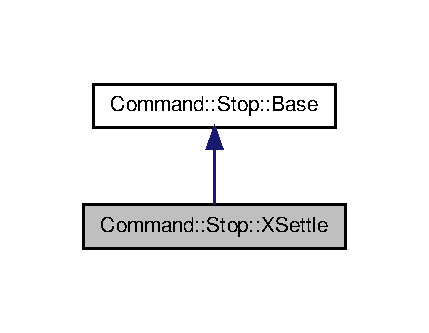
\includegraphics[width=206pt]{classCommand_1_1Stop_1_1XSettle__inherit__graph}
\end{center}
\end{figure}


\-Collaboration diagram for \-Command\-:\-:\-Stop\-:\-:\-X\-Settle\-:\nopagebreak
\begin{figure}[H]
\begin{center}
\leavevmode
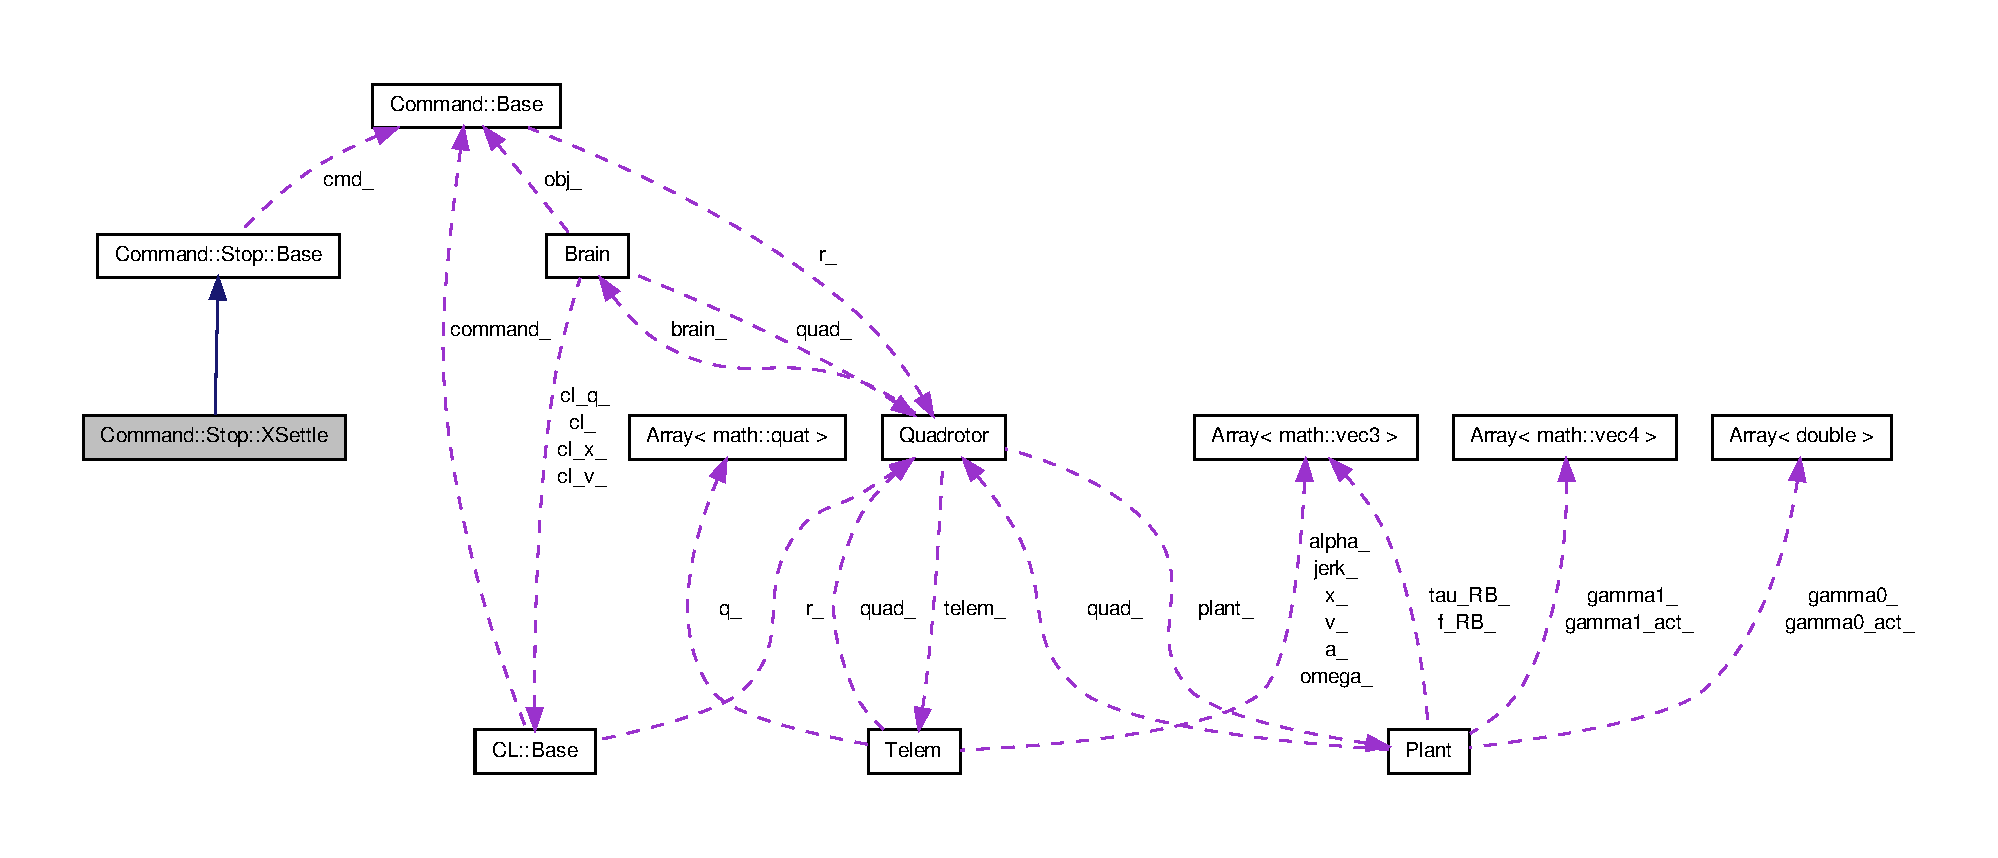
\includegraphics[width=350pt]{classCommand_1_1Stop_1_1XSettle__coll__graph}
\end{center}
\end{figure}
\subsection*{\-Public \-Member \-Functions}
\begin{DoxyCompactItemize}
\item 
\hypertarget{classCommand_1_1Stop_1_1XSettle_aacbc62cb356f0441f910e837b2cd0889}{{\bfseries \-X\-Settle} (\hyperlink{classCommand_1_1Base}{\-Command\-::\-Base} $\ast$cmd, math\-::vec3 e)}\label{classCommand_1_1Stop_1_1XSettle_aacbc62cb356f0441f910e837b2cd0889}

\item 
\hypertarget{classCommand_1_1Stop_1_1XSettle_a60ea7a816a7ea0d656551aa84a484d4d}{virtual void {\bfseries \-Check} (int)}\label{classCommand_1_1Stop_1_1XSettle_a60ea7a816a7ea0d656551aa84a484d4d}

\end{DoxyCompactItemize}
\subsection*{\-Public \-Attributes}
\begin{DoxyCompactItemize}
\item 
\hypertarget{classCommand_1_1Stop_1_1XSettle_a96f016552eec74ab167d3e0c663a8733}{math\-::vec3 {\bfseries e\-\_\-}}\label{classCommand_1_1Stop_1_1XSettle_a96f016552eec74ab167d3e0c663a8733}

\end{DoxyCompactItemize}


\-The documentation for this class was generated from the following files\-:\begin{DoxyCompactItemize}
\item 
src/quadrotor/command/\-Stop.\-hpp\item 
src/quadrotor/command/\-Stop.\-cpp\end{DoxyCompactItemize}

\printindex
\end{document}
